%Document vide aux normes de l'École nationale des Chartes
%crée par J.B. Camps
%Dernières modifications E. Rouquette (03/2025)

%%%%%%%%%%%%%%%%%%%%%% PRÉAMBULE


%%%%%%%%%%%%%% partie obligatoire du préambule
\documentclass[12pt,twoside]{book}
\usepackage{fontspec}
\usepackage{xunicode}
\usepackage{polyglossia}
\setmainlanguage{french}%indiquer la langue principale du document
%\setotherlanguage{} %indiquer les autres langues utilisée


%%%%%%%%%%%%%%%%%%%%%%%%%%%%%%%%% PACKAGES UTILISÉS

\usepackage{csquotes} % les guillemets français
\usepackage{lettrine} %faire une lettrine (pas obligatoire)

\usepackage[style=biblatex-enc/enc,sorting=nyt,maxbibnames=10]{biblatex}%charger le style de l'EnC (téléchargeable ici https://ctan.org/pkg/biblatex-enc)
\addbibresource{bibliographie.bib} %le fichier bibliograhique. Exemple de chemin à partir du dossier où se trouve le document maître:Exemple ./dossierA/fichier.bib
%\defbibheading{}{\subsection*{}} Si l'on veut changer le titre de la/les bibliographie(s)

%%%Faire un ou plusieurs index

%\usepackage{imakeidx} %pour faire un ou plusieurs index
%\makeindex %commande pour générer l'index


%RAJOUTEZ ICI VOS PACKAGES
\usepackage{minted}
\usepackage{float}
\usepackage{pgfplotstable}
\usepackage{longtable}
\usepackage{booktabs}

% Paramètres pour les blocs de code
\setminted{
    frame=lines,       % cadre autour du code
    linenos,           % numéroter les lignes
    fontsize=\small,   % taille de la police
    breaklines=true,   % couper les lignes trop longues
    breakautoindent=true, % respecter l'indentation après un saut
    breakanywhere=true % autoriser le saut n'importe où si nécessaire
}


%%%%%%%%%%%%%%%%%%%%%%%%%%%%%%%%% CONFIGURATION DE MISE EN PAGE

%%%%%% Les compteurs (sections, subsections, etc)


%%%%%% Les compteurs (sections, subsections, etc)
\renewcommand{\thesection}{\Roman{section}.}%On ne fait apparaître que le numéro de la section
\renewcommand{\thesubsection}{\arabic{subsection}.}%subsection en chiffres arabes
\renewcommand{\thesubsubsection}{\alph{subsubsection}.}%subsubsection en lettres minuscules
%Si l'on veut faire apparaître les subsubsection dans le table des matières (à commenter sinon)
\setcounter{tocdepth}{3}
\setcounter{secnumdepth}{3}  % La subsubsection (profondeur=3 dans la table des matières) apparait numérotée dans la TdM



%%%%%  Configurer le document selon les normes de l'école

\usepackage[margin=2.5cm]{geometry} %marges
\usepackage{setspace} % espacement qui permet ensuite de définir un interligne
\onehalfspacing % interligne de 1.5
\setlength\parindent{1cm} % indentation des paragraphes à 1 cm


%%%%% Mise en forme des headers (haut de page)

\usepackage{fancyhdr} %package utilisé pour modifier les headers
\pagestyle{fancy} %utiliser ses propres choix de mise en page et non ceux par défaut du package

\setlength\headheight{16pt}%la hauteur des headers

%%la façon dont les sections apparaissent dans les en-tête:

\renewcommand{\sectionmark}[1]{\markright{\small\textit{\thesection~\  #1}}}%Faire apparaître dans les headers les sections en  petit et en italiques
%\renewcommand{\sectionmark}[1]{}%Commenter la lign précédetne et mettre celle-ci pour ne pas avoir le titre des sections dans le header

%% réglages propres à frontmatter

\appto\frontmatter{\pagestyle{fancy}%
	\renewcommand{\chaptermark}[1]{\markboth{\small\textit{#1}}{}}% ne pas faire apparaître de <<numéro>> de chapitre dans les chapitres non numérotés (front: l'introduction, els remerciement, etc)
}

%% réglages propres à mainmatter

\appto\mainmatter{
\renewcommand{\chaptermark}[1]{\markboth{\small\chaptername~\thechapter~--\ \textit{#1}}{}}%faire apparaître dans les headers les sections en  petit et en italiques
%\renewcommand{\chaptermark}[1]{}%Commenter la ligne précédente et mettre celle-ci pour ne pas avoir le titre des chapitres  dans le header
}

%% réglages propres aux annexes

\appto\appendix{
	\renewcommand{\chaptermark}[1]{\markboth{\small~Annexe \thechapter~--\ \textit{#1}}{}}%faire apparaître dans les headers le nom des annexes
	%\renewcommand{\chaptermark}[1]{}%Commenter la ligne précédente et mettre celle-ci pour ne pas avoir le titre des chapitres  dans le header
}




%indiquer des règles d'hyphénation pour des mots précis si besoin
%\begin{hyphenrules}{french}
%	\hyphenation{}
%\end{hyphenrules}


%%%%%%% Package hyperref

% A mettre après les autres appels de packages car redéfinit certaines commandes).

\usepackage[xetex, colorlinks=false, breaklinks=true, pdfusetitle, pdfsubject ={Mémoire HN}, pdfkeywords={les mots-clés}]{hyperref} %
\usepackage[numbered]{bookmark}%va avec hyperref; marche mieux pour les signets. l'option numbered: les signets dans le pdf sont numérotés

% Compléter pdfsubjet et pdfkeywords
%Explication des options de hyperref (modifiables)
% hyperindex=false
% colorlinks=false: pour que le cadre des liens n'apparaisse pas à l'impression
% breaklinks permet d'avoir des liens allant sur pusieurs lignes
%pdfusetitle: utiliser \author et \title pour produire le nom et le titre du pdf


%avec overleaf, utiliser :
\hypersetup{
		pdfauthor = {Pierre Husson},
		pdftitle = {Indexation iconographique et intelligence artificielle. Expérimentations autour du Répertoire des tableaux italiens dans les collections publiques françaises (RETIF)},
		pdfsubject = {sujet},
		pdfkeywords = {Histoire de l'art} {peinture} {intelligence artificielle} {vision par ordinateur}
	}

%%%%%%%%%%%%%%%%%%%% Package glossaries

%Exception: il faut le charger APRÈS hyperref
%\usepackage[toc=true]{glossaries}
%\makeglossaries
%avec TexStudio: F9 pour compiler le glossaire (s'il y a aussi un index)

%mettre les entrées du glossaire ici ou les mettre dans un fichier à part que l'on appelle ici par \loadglsentries{nom_du_fichier.tex}

%Structure d'une entrée de glossaire
%\newglossaryentry{}{%
%	name={},%
%	description={}
%}



%%%%%%%%%%%%%%%%%% DÉFINITION DES COMMANDES ET ENVIRONNMENTS

\newcommand{\PrenomAuteur}{Pierre}
\newcommand{\NomAuteur}{Husson}
\newcommand{\Auteur}{\PrenomAuteur\ \NomAuteur}
\newcommand{\TitreMemoire}{Indexation iconographique et intelligence artificielle}
\newcommand{\SousTitreMemoire}{Expérimentations autour du Répertoire des tableaux italiens dans les collections publiques françaises (RETIF)}

 %%%%%%%%%%%%%% INFORMATIONS POUR LA PAGE DE TITRE
 
\author{\PrenomAuteur \textsc{\NomAuteur} - M2 TNAH}
\title{\TitreMemoire}

%%%%%%%%%%%%%%%%%%%%%% DOCUMENT
\begin{document}
	\begin{titlepage}
		\begin{center}
			
			\bigskip
			
			\begin{large}				
				ÉCOLE NATIONALE DES CHARTES\\
				UNIVERSITÉ PARIS, SCIENCES \& LETTRES
			\end{large}
			\begin{center}\rule{2cm}{0.02cm}\end{center}
			
			\bigskip
			\bigskip
			\bigskip
			\begin{Large}
				\textbf{\Auteur}\\
			\end{Large}
		%selon le cas
			\begin{normalsize}
				\textit{diplômé de master}
			\end{normalsize}
			
			\bigskip
			\bigskip
			\bigskip
			
			\begin{Huge}
				\textbf{\MakeUppercase{\TitreMemoire}}\\
			\end{Huge}
			\bigskip
			\bigskip
			\begin{LARGE}
				\textbf{\SousTitreMemoire}\\
			\end{LARGE}
			
			\bigskip
			\bigskip
			\bigskip
			\begin{large}
			\end{large}
			\vfill
			
			\begin{large}
				Mémoire 
				pour le diplôme de master \\
				\enquote{Technologies numériques appliquées à l'histoire} \\
				\bigskip
				2025
			\end{large}
			
		\end{center}
	\end{titlepage}

	\thispagestyle{empty}	
	\cleardoublepage
	
\frontmatter

	\chapter{Résumé}
\medskip
	Résumé du mémoire en français. Cette page ne doit pas dépasser une page.\\
	
	\textbf{Mots-clés:} une liste de mots-clés~; séparés par des points-virgules.
	
	\textbf{Informations bibliographiques:} {\Auteur}, \textit{\TitreMemoire. \SousTitreMemoire}, mémoire de master \enquote{Technologies numériques appliquées à l'histoire}, dir. Ségolène Albouy, École nationale des chartes, 2025.
	
		\newpage{\pagestyle{empty}\cleardoublepage}
	
	\chapter{Avant-Propos}

    \lettrine{C}e mémoire s’inscrit dans le cadre d’un stage mené conjointement à l’Institut national d'histoire de l'art et au sein du consortium Huma-Num pictorIA, au cours de ma seconde année de Master 2 « Technologies numériques appliquées à l’histoire » à l’École nationale des Chartes. L’objectif principal de ce stage était l’indexation iconographiques de peintures issues du RETIF (Répertoire des tableaux italiens dans les collections publiques françaises) à l’aide d’outils d’intelligence artificielle. Ce projet, intitulé \textit{Iconographia}, s’est déroulé sur une période de quatre mois, du 1\textsuperscript{er} avril au 31 juillet 2025, sous la direction de Federico Nurra et de Julien Schuh. J’ai été chargé de cette mission en raison de ma double formation en histoire de l’art et en technologies numériques. Diplômé du deuxième cycle de l’École du Louvre en 2023, j'avais consacré mes recherches à la gravure d’interprétation en Italie à l’Époque moderne, ce qui a nourri mon intérêt pour l’histoire de la peinture italienne et enrichi mes connaissances dans ce domaine. Au cours de ce projet, j’ai abordé la question principalement sous l’angle de l’historien de l’art, étant la seule personne à travailler à temps plein pour le mener. Il convient toutefois de préciser que, malgré mon intérêt pour les technologies d’intelligence artificielle, ma maîtrise des modèles d’apprentissage profond et de leurs usages reste partielle. Cette limite a entraîné certaines difficultés à manipuler ces technologies, que je présenterai au fil des chapitres. Loin de constituer un simple frein, elles ont ouvert de nouvelles perspectives et permis d’apporter un regard neuf aux pratiques d’indexation iconographique.

Je tiens tout d’abord à exprimer ma gratitude à ma directrice de mémoire, Ségolène Albouy, qui m’a accompagné tout au long de sa rédaction, et à Gennaro Toscano de présider mon jury de soutenance. Je remercie chaleureusement Federico Nurra et Julien Schuh pour leur encadrement au cours de ce stage, ainsi que mes collègues à l’INHA, Pierre-Yves Laborde, Jean-Christophe Carius, Margaux Faure, Maria Francesca Bocchi et Natacha Grim pour leurs conseils et leur soutien. Ma reconnaissance va également à mes collègues stagiaires et amis Camille Samsa, Fantin Le Ber et Mathieu Taybi, ainsi qu’à l’ensemble de mes camarades de master, pour les échanges stimulants que nous avons partagés. Je remercie également Marion Charpier et Emmanuelle Bermès pour leur accompagnement. J’adresse un merci particulier à Teoman Akgönül et Agathe Ménétrier, pour leur disponibilité et leur écoute, ainsi qu’à Johanna Daniel, dont les réflexions ont enrichi les miennes. Je voudrais témoigner ma gratitude envers Hans Brandhorst et Etienne Posthumus d'avoir accepté de s'entretenir avec moi au début de mes recherches. Enfin, je souhaite remercier mes amis et ma famille pour leur présence et leur soutien constant : Eléa Dargelos, Solveig d’Aboville, Grégoire Hignard, Thaïs Wsevoloski, Mathieu Darrieutort, Théophile Piquemal-Tabou et Inès Hennequin. Pour leur aide dans la relecture de ce mémoire, j'adresse un merci particulier à ma maman et à Adèle Bugaut. 

	\newpage{\pagestyle{empty}\cleardoublepage}
	
%%%%%%%%%%%% \bibliographie (selon les normes de l'EnC)
\printbibliography

	
\chapter{Introduction}	
En 1985, le Musée d’Art et d’Histoire de Genève accueillait de nombreux documentalistes, bibliothécaires et historiens de l’art réunis autour d’un même enjeu : réfléchir à l’avenir des collections iconographiques et à leur indexation au sein des institutions patrimoniales\footcite{rouitLecouteLoeilCollections1989}. Ce séminaire, intitulé "À l’Écoute de l’œil", plaçait l’informatisation au cœur des débats, à une époque où celle-ci commençait à transformer en profondeur les bibliothèques, les musées et les archives. Si les participants accueillaient ces innovations avec prudence, ils pressentaient déjà les perspectives considérables qu’elles offraient pour la découvrabilité des collections iconographiques, grâce à l’indexation et à leur mise à disposition du public. L’historien de l’art et professeur au Collège de France Jacques Thuillier soulignait même, de manière précoce, le rôle que pourrait jouer la recherche en intelligence artificielle pour interroger un jour de vastes banques d’images en langage naturel\footcite[p. 261]{thuillierImageInformatiqueLutilisation1989}.

Par « intelligence artificielle », on désigne aujourd'hui l’ensemble des théories et techniques permettant de concevoir des programmes informatiques capables de simuler certains aspects de l’intelligence humaine, tels que le raisonnement ou l’apprentissage. Quarante ans plus tard, l’intelligence artificielle s’invite dans tous les secteurs d’activité et s’impose comme une nouvelle révolution technologique, porteuse de perspectives comparables à celles qu’avait ouvertes l’informatisation. Depuis le début des années 2020, le déploiement de modèles de vision par ordinateur auprès du grand public a favorisé l’émergence de nombreux projets explorant l’analyse automatisée d’images. Ces modèles reposent sur des algorithmes capables de détecter, analyser, reconnaître et interpréter des éléments visuels, de manière analogue à la perception humaine.

Dans les institutions patrimoniales, ils sont de plus en plus envisagés comme des outils susceptibles d’accélérer et d’enrichir les pratiques documentaires d’indexation iconographique, contribuant ainsi à améliorer la découvrabilité des collections. Selon l’AFNOR, l’indexation est la "représentation par les éléments d'un langage documentaire ou naturel, des notions résultant de l'analyse du contenu d'un document en vue d'en faciliter la recherche"\footcite[vol. 1, p. 292]{associationfrancaisedenormalisationDocumentationRecueilNormes1993}. Dans le cas de l’indexation iconographique des œuvres d’art, il s’agit donc de recourir à des descripteurs pour décrire les scènes et les éléments représentés dans une image.

C’est dans cette dynamique qu’a vu le jour le projet intitulé textit{IconographIA}, porté par l’Institut National d’Histoire de l’Art (INHA) et le consortium Huma-Num PictorIA. Son objectif est d’appliquer des modèles de vision par ordinateur aux peintures du textit{Répertoire des tableaux italiens dans les collections françaises} (RETIF), afin d’en produire une indexation à l’aide du thésaurus iconographique Garnier pour faciliter les recherches sur le portail AGORHA.

Ce projet s’inscrit dans une réflexion plus ancienne visant à utiliser les outils informatiques pour analyser et décrire les représentations au sein des tableaux. Dès leur apparition, les thésaurus iconographiques avaient été pensés pour un usage informatisé. Les premières réflexions commencent sans doute dans les années 1960, au moment où Henri van de Waal, créateur du système de représentation iconographique textit{Iconclass}, réfléchissait déjà à l'utilisation de son système par ordinateur\footcite{vandewaalSystemeClassificationIconographique1969}. Le Metropolitan Museum of art de New York organisait alors, avec le soutien d’IBM, une conférence intitulée \textit{Computers and their potential applications in museums}, où la question de l’informatisation et de l’indexation des catalogues muséaux étaient au centre du débat\footcite{metropolitanmuseumofartComputersTheirPotential1968}. Dix ans plus tard, les réflexions se poursuivaient à Pise, d’abord en 1968 lors de la \textit{First international conference on automatic processing of art history data and documents}\footcite{barocchiFirstInternationalConference1978} puis lors de la seconde édition en 1984\footcite{cortiAutomaticProcessingArt1984}. La même année, le Thésaurus iconographique Garnier était publié, avec la volonté d’uniformiser la pratique documentaire en vue d’une mise en commun des bases de données muséales en France. L’année suivante, Florin Coman soutenait sa thèse intitulée "Histoire de l'art et informatique documentaire", publiée plus tard en 1988\footcite{comanLhistoireLartLinformatique1988}, et le séminaire "À l'Écoute de l'Oeil", que nous évoquions plus avant, discutait des enjeux de l'informatique pour les collections iconographiques\footcite{rouitLecouteLoeilCollections1989}. En dépit de ces initiatives, les technologies numériques ont tardé à être intégrées dans les pratiques d’histoire de l’art et à être acceptées par la communauté des chercheurs, comme le soulève Jacques Thuillier en 1992 : “un quart de siècle d’informatique n’a rien changé aux habitudes de l’histoire de l’art, tant internationale que française [...] l’échec n’est pas à mettre au compte de l’informatique, mais des historiens de l’art, qui n’ont pas su tirer parti d’elle.”\footcite[p. 5]{thuillierLinformatiqueHistoireLart1992}. Cinq ans plus tard, peu après l’apparition d’internet en France, le même auteur déplore la latence que prend la mise en ligne des bases de données liées au patrimoine, comme Joconde et Mérimée.\footcite[p. 8]{thuillierLinformatiqueLhistoireLart1997}. Les deux décennies suivantes voient l’accélération de la mise en ligne des contenus patrimoniaux, et la multiplication des projets numériques. Cependant, l’intelligence artificielle, telle qu’on la conçoit aujourd’hui, n’apparaît en histoire de l’art qu’au cours des années 2010, et surtout au début des années 2020. Dans le domaine de l’analyse des peintures, les projets et publications se sont multipliés ces dernières années. Les expérimentations menées par Benoît Seguin dans le cadre du projet \textit{Replica}, en collaboration avec la fondation Cini à Venise et dont les premiers résultats ont été publiés en 2016\footcites{seguinVisualLinkRetrieval2016}{dilenardoVisualPatternsDiscovery2016}, ainsi que des initiatives comme le projet international \textit{Augmented Artwork Analysis} (AAA)\footcite{AugmentedArtworkAnalysis}, fondé en 2021, mobilisent les outils de vision par ordinateur pour approfondir l’étude des peintures. Parallèlement, les nombreuses recherches conduites par David G. Stork sur l’analyse par ordinateur d’œuvres picturales ont abouti à une synthèse de référence sur le sujet\footcite{storkPixelsPaintingsFoundations2024}, soulignant le potentiel et les défis de ces approches dans le champ des études artistiques. Les revues spécialisées et les rencontres académiques ont contribué à alimenter la réflexion sur le sujet, comme en témoigne le numéro 87 de la revue \textit{Histoire de l’art} paru en 2021, consacré aux Humanités numériques et incluant un échange modéré par Mathieu Aubry avec Lisandra Costiner et Stuart James sur les implications de l'intelligence artificielle dans la discipline\footcite{aubryArtificialIntelligenceArt2021}. L’indexation iconographique occupe une place croissante dans les réflexions sur l’usage de ces outils numériques. De nombreux projets visent à tirer parti de ces pratiques documentaires pour améliorer la gestion et la découvrabilité des collections. En 2019, Hans Brandhorst proposait une analyse des implications conjointes d’Iconclass et de l'intelligence artificielle\footcite{brandhorstWordWorthThousand2019}, tandis que des institutions telles que le Musée national des Arts Asiatiques – Guimet\footcite{HikarIA} ou le Musée des Arts décoratifs\footcite{bermesRepenserCollectionsPatrimoniales2025} ont développé des projets visant à enrichir la connaissance de leurs fonds grâce aux technologies de vision par ordinateur.

Le projet IconographIA s'inscrit dans ces réflexions en soulevant plusieurs questions liées à l’intégration des outils d’intelligence artificielle dans la pratique de l’indexation iconographique des œuvres picturales. Comment ces technologies peuvent-elles enrichir la connaissance et l’étude de ces collections ? Quels défis méthodologiques, sémantiques et techniques soulève l’intégration des systèmes d'apprentissage profond dans la description des représentations ? Quel rôle jouent les vocabulaires contrôlés dans ce processus, et comment assurer l’interopérabilité entre les algorithmes de vision par ordinateur et ces référentiels normés comme le thésaurus Garnier ?
Dans un premier temps, il convient d'examiner les pratiques d’indexation et leurs enjeux, les vocabulaires employés ainsi que leur intégration dans les projets numériques et les bases de données. Cette analyse permet ensuite de réfléchir à la possibilité d’automatiser ce processus, en considérant les aspects techniques et méthodologiques et en identifiant les méthodes les plus pertinentes. Les avantages et limites d’une telle automatisation seront également discutés. Enfin, la réflexion s’élargit aux alternatives à l’automatisation, en explorant d’autres approches de vision par ordinateur susceptibles de faciliter le travail de l’indexeur, tout en permettant de nouvelles perspectives d’exploration des corpus d’images.


\newpage{\pagestyle{empty}\cleardoublepage}

%%%%%%%%%%%%%%%%%Le corps du mémoire
	\mainmatter
%Trier par dossiers si besoin (front, main,annexes,), se crérer un docuemnt .tex par structure (section ou chapter selon la taille et la pertinence) Exemple de chemin à partir du dossier où se trouve le document maître: ./dossierA/fichier.tex

	

	\part{L’indexation iconographique des œuvres patrimoniales à l’ère du numérique}

\chapter[Indexation : principes et enjeux]{Principes et enjeux de l’indexation iconographique en histoire de l’art}
\section{L'indexation iconographique en histoire de l’art}

Bien que la pratique de l’indexation remonte à plusieurs siècles,ce n’est qu’à partir du milieu du XX\textsuperscript{e} siècle qu’elle a fait l’objet d’une véritable théorisation, notamment pour la description du contenu intellectuel des livres et des documents conservés dans les bibliothèques\footnote{Consulter à ce propos : \cite{amarFondementsTheoriquesLindexation2000}.}. Lorsqu’elle s’applique aux objets muséaux, cette méthode reprend les principes développés pour les textes, tout en les enrichissant par les apports de l’archéologie et de l’histoire de l’art, indispensables à leur compréhension et à leur interprétation.

Pour définir et expliciter la pratique de l’indexation dans la pratique documentaire du catalogage, l'Association française de normalisation (AFNOR) la présente ainsi : l’indexation est « l’opération qui consiste à décrire et à caractériser un document à l’aide de représentations des concepts contenus dans ce document, c’est-à-dire à transcrire en langage documentaire les concepts après les avoir extraits du document par une analyse. La transcription en langage documentaire se fait grâce à des outils d’indexation tels que thésaurus, classifications, etc. […] La finalité de l’indexation est de permettre une recherche efficace des informations contenues dans un fonds de documents et d’indiquer rapidement, sous une forme concise, la teneur d’un document \footcite[norme NF Z47-102, vol. 1, p. 286]{associationfrancaisedenormalisationDocumentationRecueilNormes1993} ». L’indexation iconographique, en histoire de l’art, constitue une application spécifique de ce principe : elle consiste à décrire le contenu des images à l’aide de descripteurs afin de faciliter l’accès aux œuvres, sans cependant dispenser sa consultation\footnote{« Le rôle du système de recherche documentaire est de faciliter l’accès au document et non de dispenser sa consultation » \cite[p. 15]{garnierThesaurusIconographiqueSysteme1984}.}. Avec le développement des bases de données, ces pratiques d’indexation reposent désormais presque systématiquement sur des vocabulaires contrôlés pour décrire les documents. Pour les œuvres d'art, où peuvent être présentés des objets, des personnages, mais aussi des concepts ou des scènes souvent codifiées, les thésaurus jouent un rôle central pour décrire ces éléments de manière normalisée. Ainsi, les méthodes et manuels d’indexation sont fréquemment associés aux thésaurus qu’ils accompagnent, afin de garantir une utilisation la plus uniforme possible du vocabulaire et d'assurer l’efficacité des recherches qui en découlent. Les principaux systèmes d’indexation iconographique, tels qu’\textit{Iconclass} et le thésaurus Garnier, sont chacun accompagnés d’études et de guides destinés à encadrer leur utilisation, fournissant également des réflexions sur cette pratique documentaire\footnote{Nous décrirons plus en détail l'histoire, l'utilisation et les particularités de ces thésaurus dans le chapitre 2.}.

Cependant, les recommandations concernant l’usage des thésaurus ne fournissent pas une méthode claire et rigoureuse pour l’indexation des images, et ce pour plusieurs raisons. La première est le manque d’études consacrées à cette pratique en histoire de l'art. Certaines études comme celles de Sarah Shatford prennent en considération toutes les images et restent trop génériques pour des œuvres picturales\footcites{shatfordDescribingPictureThousand1984}{shatfordAnalyzingSubjectPicture1986}. Dans son manuel sur l’usage du système iconographique \textit{Iconclass} publié en 1994, l'historien d'art Roelof van Straten remarque que la communauté scientifique s’est rarement penchée sur des questions pourtant essentielles liées à l’indexation, telles que la nature même de la tâche de l’indexeur ou la profondeur à laquelle l’indexation doit être effectuée.\footnote{\cite{vanstratenIconographyIndexingIconclass1994}, p. 37 : “It is astonishing that even the most basic questions regarding iconographic indexing, such as “What is the real task of the iconographic indexer?” or “How far ‘in depth’ should we index ?” do not seem to have been discussed among art historians.”}. Une autre raison est celle de la grande variété des images à indexer présente dans les institutions patrimoniales ou les collections, rendant difficile l’écriture d’une méthode efficace. François Garnier, dans l'introduction de son thésaurus iconographique utilisé par les musées français, indique alors « qu'aucune grille d'analyse ne s'impose comme une nécessité »\footcite[p. 25]{garnierThesaurusIconographiqueSysteme1984}. 

S’il n’existe pas de consensus sur la manière de rédiger une indexation « parfaite » pour décrire une image, ces auteurs soulignent que l’indexeur doit avant tout se laisser orienter par la finalité de sa tâche : permettre un accès efficace aux images au sein d’une base de données et faciliter les recherches, présentes comme futures, des analystes d’images. Ils proposent à cet effet une liste d’éléments essentiels à prendre en compte pour décrire une représentation\footnote{\cite[p. 57-58]{vanstratenIconographyIndexingIconclass1994}, \cite[p. 25]{garnierThesaurusIconographiqueSysteme1984}}. Cette description doit d’abord rendre compte de la signification principale de l’image et de son contenu, en identifiant la scène, les personnages et les lieux représentés. Elle doit ensuite être enrichie par le relevé des motifs secondaires, liés ou non à l’action principale. Une attention particulière doit être portée aux éléments inhabituels, surtout lorsqu’ils présentent un intérêt historique, ainsi qu’aux détails que l’image met en avant. L’objectif est surtout de restituer autant de concepts du contenu visuel que possible, même s’il existe toujours une part inévitable de subjectivité dans le travail d’indexation. Sara Shatford insiste également sur le besoin d’être concis pour éviter de fausser les recherches dans les bases de données et d’abord privilégier les idées les plus importantes, en fonction du public visé\footcite{shatfordDescribingPictureThousand1984}. La qualité de l’indexation dépend également de plusieurs paramètres : la qualité du système d’indexation utilisée et sa compréhension par l’indexeur, l’expérience et les connaissances de ce dernier, et la lisibilité de l’image\footnote{\cite[p. 24]{garnierThesaurusIconographiqueSysteme1984}, \cite[p. 37]{vanstratenIconographyIndexingIconclass1994}}.

\section{Sujets, genre, motifs et éléments}

L’usage du vocabulaire générique que nous emploierons tout au long de ce mémoire pour décrire les images ne fait pas l’objet d’un accord unanime chez les historiens de l’art\footnote{Nous avons consulté à ce propos différents ouvrages généralistes qui abordent le vocabulaire : \cite{vanstratenIntroductionIconography1994}, \cite{barralialtetDictionnaireCritiqueDiconographie2003}, \cite{bergeonlanglePeintureDessinVocabulaire2009}, \cite{gervereauVoirComprendreAnalyser2020}.}. Les termes « motifs », « thèmes », « sujet », « genre » et « éléments » ne sont pas toujours employés dans le même sens en fonction des publications. C’est pourquoi nous exposons ici la manière dont nous utiliserons ces termes. 

Le terme « sujet » désigne le thème représenté dans une image ou une œuvre d’art, c’est-à-dire l’objet principal de la représentation. Il peut se référer au sujet général, correspondant à la catégorie de la représentation (portrait, paysage, scène religieuse ou mythologique), ou à une scène spécifique, c’est-à-dire une situation particulière représentée. Le sujet sert souvent à formuler le titre d’une œuvre lorsqu’aucun titre n’a été donné par l’artiste ou forgé par l’historiographie. Dans ce cas, nous préférons utiliser le terme « scène » pour plus de précision.

Dans l’histoire de la peinture, le sujet général, également appelé « genre », relève d’une classification théorisée dès le XVIIᵉ siècle. Dans son introduction aux conférences de l’Académie royale de peinture en 1667, André Félibien définit plusieurs genres iconographiques selon une hiérarchie\footnote{felibienConferencesLAcademieRoyale1667} : la peinture d’histoire, qui occupe le premier rang, regroupe les œuvres représentant des événements historiques ou illustrant des textes, tels que la Bible ou la mythologie grecque et romaine. Le portrait constitue le deuxième genre pictural, suivi de la scène de genre, qui représente des scènes anecdotiques ou familières, souvent inspirées du quotidien. Viennent ensuite les genres qui mettent moins l’accent sur la figure humaine : le paysage, puis la nature morte, centrée sur la représentation d’éléments inanimés. Cette classification a profondément marqué l’histoire picturale, en particulier à l’Époque moderne. Si elle a désormais perdu son caractère hiérarchique, elle reste prégnante aujourd’hui dans les thésaurus comme les dictionnaires, avec quelques adaptations pour refléter la diversité de certaines catégories, en particulier la peinture d’histoire, et pour intégrer des genres apparus ultérieurement, comme la peinture abstraite.

Le « motif » désigne quant à lui un élément visuel particulier, un détail significatif ou un groupe d’éléments dans une œuvre, qui peut être isolé ou répété, et parfois associé à d’autres. Il peut être figuratif ou décoratif, notamment dans le cas de motifs ornementaux. 

Enfin, un « élément » est la plus petite unité significative identifiable dans une image. Il peut s’agir d’une figure, d’un détail, d’un objet spécifique, d’un attribut iconographique ou d’une partie d’un motif paysager ou architectural.

Pour éclaircir ces notions, la description sommaire d’un tableau peut servir d’illustration. Prenons l’\textit{Adoration des bergers} peinte à tempera sur bois par le peintre florentin Taddeo Gaddi (vers 1300-1366) vers 1330 et conservé au Musée des Beaux-Arts de Dijon (inv. 1470) (figure \ref{fig:ptrGaddiAdoration}). Elle relève d’un \textit{sujet} biblique, puisque la \textit{scène} représentée provient du Nouveau Testament, plus particulièrement de l’Évangile selon saint Luc (chapitre 2, versets 8-20). Dans l’image, plusieurs \textit{motifs} peuvent être identifiés, comme les bergers, la Vierge tenant l’Enfant Jésus dans ses bras ou encore saint Joseph se reposant en bas à droite de la composition. Le bâton du berger au centre du panneau, l’auréole de la vierge ou la fenêtre visible sur le mur du bâtiment peuvent être désignés comme des \textit{éléments}.

\section[Iconographie et Iconologie]{La lecture de l'image :  Iconographie et Iconologie}

L’analyse des images en histoire de l’art, en particulier par l’identification de leurs thèmes et des scènes représentées, constitue un champ d’étude spécifique, appelé iconographie. La définition et la méthode proposées par l’historien de l’art Erwin Panofsky (1892-1968) dès 1931 sont régulièrement citées pour définir cette discipline\footnote{Erwin Panofsky la définit pour la première fois en 1931 lors d’une conférence à Kiel auprès de la société d’études kantiennes : \cite{panofskyProblemBeschreibungUnd1932}. Il affine ensuite cette définition dans l'introduction de ses \textit{Studies in Iconology} publiés en 1939 puis dans \textit{Meaning in the visual arts} publié en 1955.}. Il définit l’iconographie comme « cette branche de l’histoire de l’art qui se rapporte au sujet ou à la signification des œuvres d’art, par opposition à leur forme »\footcite[p. 19]{panofskyEssaisDiconologieThemes2021}. Plus précisément, le terme iconographie revêt deux sens complémentaires : le premier désigne l’ensemble des représentations d’un même sujet ou thème dans les arts visuels ; le second correspond à la discipline d’histoire de l’art elle-même, centrée sur l’identification, la description et l’interprétation du contenu des images, en examinant les sujets représentés, les compositions, et tous les éléments distincts du style. Ce dernier terme, que Panofsky désigne comme “la forme”, recouvre les qualités plastiques de la représentation, notamment les lignes, les couleurs, la composition, les proportions, les volumes ou encore la lumière. L’iconographie s’intéresse ainsi essentiellement au contenu narratif ou symbolique des œuvres, plutôt qu’à leur aspect formel. 

Le terme d’iconologie est généralement employé en complément de l’iconographie. Les historiens font remonter cette notion, dans son acception proche de son usage contemporain, à Cesare Ripa, érudit italien, qui publie en 1593 un manuel intitulé \textit{Iconologia}\footcite{ripaIconologia1593}, largement diffusé au XVIIᵉ siècle. Cet ouvrage servait de dictionnaire destiné à expliquer la manière de représenter et reconnaître les personnifications et allégories, en précisant leurs attributs\footnote{Voir à ce sujet \cite{okayamaRipaIndexPersonifications1992}}. Comme le souligne Xavier Barral i Altet, le sens du mot iconologie comprenait alors, au moment de la parution de cet ouvrage, ce que nous désignons aujourd’hui par « iconographie »\footcite[p. 24]{barralialtetIntroduction2003}. Au XXᵉ siècle, une nouvelle approche de l’iconologie est développée à Hambourg en Allemagne autour de l’historien d’art Aby Warburg (1866‑1929), puis surtout par Erwin Panofsky, qui entend l’iconologie comme une approche destinée à interpréter le sens profond des images et à dégager leur signification symbolique, en lien avec le contexte culturel, philosophique, religieux ou social de leur création.

Ainsi, Panofsky propose une méthode en trois niveaux pour interpréter le contenu d’une image. Bien que cette démarche ait suscité certaines critiques et ajustements au cours du temps, elle reste aujourd’hui largement respectée pour avoir théorisé la pratique iconographique et iconologique\footcite[en particulier le premier chapitre «What is Iconography?», p. 3-25]{vanstratenIntroductionIconography1994}. Le premier niveau de cette méthode, la description pré-iconographique, consiste à identifier les éléments et les motifs visibles dans la représentation : figures humaines, animaux, objets et leurs relations mutuelles, y compris les événements représentés. Les qualités expressives, telles que la joie, la tristesse ou d’autres intentions, sont également relevées à cette étape. La connaissance de l’histoire du style permet de comprendre comment certains éléments sont représentés dans un contexte particulier : par exemple, un dauphin dans la tradition médiévale est figuré très différemment de la réalité. Le deuxième niveau, l’analyse iconographique, consiste à mettre en relation les motifs et compositions avec des sujets ou des thèmes précis, en identifiant les images, les scènes et les allégories représentées. Le troisième niveau, l’interprétation iconologique, vise à dégager le sens profond de l’image, souvent lié aux choix de l’artiste ou du commanditaire dans la représentation des motifs. Voici un exemple pour illustrer cette démarche : une description pré-iconographique pourrait consister à observer un vieillard levant un couteau et tenant un jeune garçon d’une main, avec un bélier à ses côtés et un ange descendant du ciel. L’analyse iconographique identifierait Abraham sacrifiant son fils, comme raconté au chapitre 22 de la Genèse. L’interprétation iconologique, selon une lecture typologique, pourrait mettre en évidence une allusion à Dieu sacrifiant son fils, préfigurant la Passion du Christ dans le Nouveau Testament. 

Comme le souligne Roelof van Straten, pour l’indexation iconographique, ce sont surtout les deux premières étapes qui importent, c’est-à-dire l’identification du sujet, des scènes, des motifs et des éléments représentés dans l’œuvre\footcite{vanstratenPanofskyICONCLASS1986}. Les conclusions issues d’une interprétation iconologique peuvent également être intégrées à l’indexation, à condition que les concepts soient précis et validés par le contexte de création ou par des sources documentaires. C’est le cas, par exemple, des \textit{Memento mori} présents dans les natures mortes, des représentations de vanités ou des paysages de l’Arcadie. Cela vaut aussi pour les préfigurations dans les associations typologiques entre l’Ancien et le Nouveau Testament.

\chapter[Les instruments de l'indexation]{Les instruments de l'indexation : vocabulaires contrôlés et systèmes d’indexation}
Comme nous l'évoquions précédemment, les méthodes d'indexation sont intimement liées aux vocabulaires qu’elles utilisent. En histoire de l'art, la plupart des vocabulaires ont vu leur naissance dans la deuxième moitié du XX\textsuperscript{e} siècle, et surtout dans les années 1980, avec le développement des systèmes informatiques dans les institutions patrimoniales et l’amélioration des pratiques de catalogage. Des vocabulaires d’indexation iconographique génériques ont alors vu le jour, destinés à décrire l’ensemble des représentations artistiques, tandis que des vocabulaires spécialisés sont employés pour un domaine d’étude précis ou un projet particulier. La question de l'alignement de ces vocabulaires est un enjeu crucial pour l'interopérabilité des bases de données et la facilitation de la recherche iconographique.

\section{Vocabulaires génériques et spécifiques}

Différents types de vocabulaires peuvent être mobilisés pour décrire les représentations présentes au sein des objets patrimoniaux, selon l’ampleur de l’analyse envisagée et le degré de spécialisation des approches adoptées. Certains sont spécifiquement liés à des domaines d’étude particuliers, tandis que d’autres, plus généralistes, visent à proposer une description uniforme des représentations, quel que soit leur contexte de création.
Ainsi, les vocabulaires spécialisés sont souvent associés à des projets de recherche ou à des disciplines précises. Pour les objets archéologiques, par exemple, le Lexicon Iconographicum Mythologiae Classicae (LIMC) constitue une référence. Publié en huit tomes doubles entre 1981 et 2009, il est consacré aux représentations figurées issues des mythologies grecque, étrusque et romaine, appliquées à divers objets antiques (céramique, sculpture, orfèvrerie, glyptique, peinture, mosaïque, etc.)\cite{fondationinternationalepourlelimcLexiconIconographicumMythologiae1981, fondationinternationalepourlelimcLexiconIconographicumMythologiae2009}. 

Dans le domaine de l’art médiéval, plusieurs répertoires et dictionnaires iconographiques ont vu le jour, parmi lesquels l’Index of Medieval Art de l’université de Princeton. Fondé en 1917 par le professeur Charles Rufus Morey, il a d’abord été conçu au format papier, rassemblant un index des iconographies chrétiennes, puis juives, islamiques et non religieuses, accompagné de photographies. Informatisé en 1991, il est accessible en ligne depuis 2017\footcite{HistoryIndex}. Plus récemment, des projets tels que l’Ontologie du christianisme médiéval en images, mise en ligne en 2023 par l’Institut national d’histoire de l’art, proposent également un lexique contrôlé pour les représentations figurées dans le contexte médiéval\footcite{beaudOntologieChristianismeMedieval2023}.
Pour les œuvres d’art picturales, il existe certes des dictionnaires spécialisés, mais ce sont surtout des systèmes iconographiques généralistes qui sont employés pour leur description. Certains ont été développés dans le cadre d’institutions, comme le système d’indexation par mots-clés du Warburg Institute\footcite{thewarburginstituteSummaryGuidePhotographic1988}, ou encore le Thesaurus for Graphic Materials, publié par la Library of Congress et principalement utilisé pour les estampes et les photographies\footnote{Aujourd’hui disponible en ligne : \cite{libraryofcongressThesaurusGraphicMaterials2024}}.

Aujourd’hui, les vocabulaires iconographiques les plus utilisés dans les institutions, notamment pour la description des œuvres d’époque moderne et contemporaine, sont \textit{ICONCLASS}, les thésaurus développés par le Getty Research Institute, et, en France, le thésaurus Garnier. Parallèlement, Wikidata prend une place croissante dans la description des représentations, grâce à l’implication grandissante de contributeurs et d’institutions qui y participent activement.

Le système iconographique Iconclass a été conçu à l’initiative de l’historien de l’art néerlandais Henri van de Waal. Publié une première fois en 1968 sous l’acronyme D.I.A.L. (textit{Decimal Index of the Art of the Low Countries})\footcite{vandewaalDecimalIndexArt1968}, il prend rapidement le nom d’Iconclass, contraction d’ICONographic CLASSification (parfois rendu ICONographic CLASsification System). Initialement prévu pour paraître en volumes imprimés, il fait l’objet d’une édition augmentée et révisée entre 1973 et 1985, comprenant sept volumes consacrés au système, sept volumes de bibliographie et trois volumes d’index\footcite{vandewaalIconclassIconographicClassification1974}. Dès le début des années 1970, Van de Waal anticipe un usage informatisé du dispositif, ce qui conduit à une collaboration avec le Centraal Rekeninstituut de Leyde et au portage d’Iconclass sur un ordinateur IBM mainframe en 1978\footcite[p. 202]{brandhorstICONCLASSKeyCollaboration2017}. Après des versions diffusées sur CD-ROM dans les années 1990, le système est finalement mis en ligne entre 1999 et 2000\footcite{brandhorstSurveyVersionsIconclass}. Le principe d’Iconclass repose sur une classification hiérarchique des représentations, organisée en dix classes principales, chacune subdivisée en catégories plus fines, couvrant notamment les domaines de la Nature, de L’Être Humain, de l’Histoire, de la Bible ou des Mythologies. Chaque concept est identifié par un code alphanumérique, dont la longueur indique le degré de précision : plus le code est détaillé, plus la description est fine.

Parallèlement aux travaux de Van de Waal, des initiatives de normalisation des vocabulaires émergent aux États-Unis, portées par le Getty Trust, puis par le Getty Research Institute (GRI), fondé en 1985. Dès la fin des années 1970, est engagé le développement de l’Art \& Architecture Thesaurus (AAT), destiné à répondre aux besoins des bibliothèques et des revues spécialisées en matière de catalogage et d’indexation\footcite{gettyresearchinstituteAAT2024}. Le projet est initié par les directeurs de bibliothèques et des historiens de l’art Toni Petersen, Dora Crouch et Pat Molholt,  avec le soutien financier du Getty Trust. Structuré au cours des années 1980 par le Getty Vocabulary Program, l’AAT paraît en deux éditions imprimées, en 1990 et 1994\footcite{petersenArtArchitectureThesaurus1990}. De portée générale, l’AAT rassemble des termes multilingues pour désigner des agents, des types d’œuvres, des rôles, des matériaux, des styles, des cultures et des techniques de création. Si certains de ces termes concernent aussi les sujets iconographiques, c’est surtout la Getty Iconography Authority (IA), intégrée au programme des vocabulaires du GRI, qui s’attache directement aux représentations iconographiques. Plus spécialisé, ce vocabulaire recense des noms propres, des personnages religieux ou fictifs, des événements historiques, ainsi que des titres d’œuvres littéraires ou de spectacles, en intégrant des relations et des repères chronologiques. L’accent est particulièrement mis sur les cultures non occidentales,  notamment asiatiques et américaines, tout en établissant des références croisées avec d’autres ressources, telles qu’Iconclass pour le contexte occidental\footcite{gettyresearchinstituteCONAIA2024}. Afin de faciliter les mises à jour régulières, une version numérique de l’AAT est mise en ligne en 1997, accompagnée d’une interface de recherche. Depuis, l’ensemble des vocabulaires Getty, dont l’AAT et l’IA, est accessible via le site du Getty Research Institute\footcite{gettyresearchinstituteGettyVocabularies}.

En France, s’est développé à la même époque le \textit{Thésaurus iconographique, système descriptif des représentations de François Garnier}, plus couramment appelé thésaurus Garnier. Initié en 1976 à la demande du Ministère de la Culture, il répondait aux besoins de l’Inventaire général des monuments et des richesses artistiques de la France ainsi qu’à ceux de la Direction des musées de France\footcite[p. 11]{garnierThesaurusIconographiqueSysteme1984}. Son objectif était de fournir une liste de descripteurs destinés à l’indexation des documents iconographiques et à l’alimentation des bases de données créées par ces services. Conçu avec une vocation universelle, ce thésaurus visait à offrir un langage normalisé permettant de décrire toute représentation, indépendamment de sa date, de sa nature ou de son support. Le thésaurus Garnier demeure aujourd’hui « l'outil retenu par le ministère de la Culture pour l'analyse des représentations figurées dans les bases de données patrimoniales » en France\footnote{\cite{ministeredelacultureThesaurusIconographiqueSysteme2020}}. La première version a été publiée sous forme d’ouvrage aux éditions Léopard d’or. Richement illustrée de reproductions de gravures sur bois accompagnées d’exemples d’indexation conforme aux règles du thésaurus, offrant ainsi aux utilisateurs des cas pratiques d’application\footcite{garnierThesaurusIconographiqueSysteme1984}. Cette version initiale se composait de quatre rubriques : une liste hiérarchisée de termes pour décrire une représentation, une liste non exhaustive de noms propres ou de termes particuliers (par exemple des lieux), les sources textuelles dont les représentations sont issues et des termes permettant de dater le contenu représenté (et non l’exécution de l’œuvre). De nombreux musées français utilisent encore cette version imprimée, désormais mise à disposition en ligne grâce à une numérisation complète réalisée par le ministère de la Culture\footcite{ministeredelacultureThesaurusIconographiqueSysteme2020}. Celui-ci propose également une version hébergée sur Opentheso, structurée en 22 catégories et comprenant 32 895 concepts\footcite{ministeredelacultureThesaurusIconographiqueGarnier}. L’Institut national d’histoire de l’art (INHA) diffuse quant à lui une version distincte, totalisant 16 362 concepts répartis en 24 catégories\footcite{institutnationaldhistoiredelartThesaurusAGORHAGarnier2021}. Enfin, le thésaurus iconographique utilisé par Mandragore, la base de données recensant les enluminures des manuscrits de la Bibliothèque nationale de France, correspond à une version dérivée et simplifiée du thésaurus Garnier\footcite{bibliothequenationaledefranceThesaurusIconographiqueMandragore2024}.

Enfin, Wikidata constitue aujourd’hui une alternative pour décrire les représentations au moyen de ses propriétés\footcite{Wikidata}. Créée en 2012 par la Wikimedia Foundation, cette base de connaissances libre et collaborative est accessible en ligne\footcite{perezWikipediasNextBig2012}. Elle fonctionne comme un référentiel sémantique où chaque entité est décrite par un élément (item), identifié par un identifiant unique. Wikidata est utilisée pour structurer et centraliser les données des projets Wikimedia (comme Wikimedia Commons ou Wikipedia), mais aussi par des institutions patrimoniales et scientifiques afin d’enrichir ou d’interconnecter leurs bases de données. Chaque élément y est défini par un label, c’est-dire le nom principal, complété d’une description et éventuellement d’alias correspondant à des variantes ou synonymes. Tous ces champs sont multilingues. Les images et les éléments peuvent être reliés entre eux grâce aux propriétés de Wikidata. Par exemple, dans le cas de la description iconographique, la propriété P180 (dépeint / depicts) permet d’associer une image à l’élément qu’elle représente\footcite{P180DepeintDepicts}.

\section{Systèmes descriptifs et systèmes d'indexation}

En 1994, Roelof van Straten faisait la distinction entre des “systèmes descriptifs” (\textit{descriptive systems}) qui utilisent uniquement du langage naturel et les “systèmes d’indexation” (\textit{indexing systems}) dont le but n’est pas de décrire les images mais de les indexer en leur attribuant un ou plusieurs codes ou mot-clés\footcite[p. 101]{vanstratenIconographyIndexingIconclass1994}. Cette distinction permet de comprendre l’utilisation des différents systèmes et vocabulaires utilisés dans la description iconographique, surtout dans le cadre de projets numériques. Avec l’apparition de l’informatisation, on observe une mutation des systèmes descriptifs en systèmes d’indexation en s’appuyant sur les technologies fournies par les outils numériques.

Par système descriptif, on entend des systèmes reposant sur le langage naturel, utilisant des mots ou des expressions pour décrire une image. Les thésaurus entrent dans cette catégorie, car ils fournissent des termes contrôlés permettant de qualifier les représentations. Le thésaurus iconographique Garnier a été conçu dans cet esprit. Dans sa version papier, il propose ainsi une liste hiérarchisée de plus de 3 200 descripteurs, répartis en 23 classes. Parmi celles-ci, 14 classes sont considérées comme fixes, tandis que les autres peuvent être adaptées à des collections particulières\footcite[p. 15]{garnierThesaurusIconographiqueSysteme1984}. Ces classes se répartissent en deux catégories principales : thèmes et sujets. Les thèmes regroupent des motifs communs, classés en 14 catégories, telles que la nature, les transports et la communication, ou les ornements. Les sujets se réfèrent à des scènes ou des personnages identifiables, issus de textes bibliques, de la mythologie, de l’histoire ou de récits. Pour représenter les relations hiérarchiques entre les éléments et les catégories, des parenthèses sont ajoutées dans les descriptions. Par exemple, pour la peinture représentant Saint Apolline et Saint Sébastien du Pérugin, conservée au Musée de Grenoble (figure \ref{fig:ptrPeruginSaints}), la description selon le thésaurus papier devait être formulée ainsi :

\begin{quote}
Groupe de figures (sainte Apolline, pince, dent, en pied, de face, Saint Sébastien, flèche).
\end{quote}

Pour la peinture de \textit{Persée délivrant Andromède} de Paul Véronèse (1528-1588) conservée au Musée des beaux-arts de Rennes (inv. 1801.1.1) (figure \ref{fig:ptrVeronesePersee}), la description iconographique pourrait être formulée ainsi :

\begin{quote}
Scène mythologique (Persée, épée, Andromède, monstre : marin, bord de mer, délivrance, rocher, chaîne) - fonds de paysage (ville)
\end{quote}

Ainsi, la description formulée s’apparente à une description formulée en langage naturel, en s’appuyant sur les termes fournis par le thésaurus. 

Quant aux systèmes d’indexation, ils n’avaient pas pour objectif de fournir une description complète des images, mais plutôt d’attribuer des mots-clés ou des codes normalisés permettant de les classer et les retrouver dans une base de données. Ils reposent sur des concepts pouvant désigner une idée, un terme, une scène, un motif ou un élément de représentation, chacun étant identifié par un code ou un mot-clé. Iconclass en constitue l’exemple le plus abouti : il utilise des codes alphanumériques qui restituent la hiérarchie du système et précisent progressivement un concept. Le premier caractère du code correspond à la catégorie la plus générale, puis les suivants affinent la description. Ainsi, le \textit{Persée délivrant Andromède} de Paul Véronèse est indexé par le code 94P211. Celui-ci indique successivement : la mythologie classique (9), les légendes héroïques grecques (94), l’histoire de Persée (P), ses amours (2) avec Andromède (1), et plus précisément l’épisode où Persée tue le monstre marin pour la délivrer (1). La notice correspondante décrit en français : « 94P211 Persée tue le monstre marin (ou le pétrifie en lui montrant la tête de Méduse) et délivre Andromède ; il se peut que les parents de celle-ci, Céphée et Cassiopée, observent la scène »\footnote{ICONCLASS 94P211, \url{https://iconclass.org/94P211}}. Dans d’autres cas, le code peut inclure un nom propre, comme pour \textit{saint Sébastien et sainte Apolline} de Pérugin (figure \ref{fig:ptrPeruginSaints}, qui serait décrit à l'aide de ces deux codes : (11H(SEBASTIAN))\footnote{ICONCLASS 11H(SEBASTIAN),  \url{https://iconclass.org/fr/11H\%28SEBASTIAN\%29}} et (11HH(APOLLONIA))\footnote{ICONCLASS 11HH(APOLLONIA), \url{https://iconclass.org/11HH\%28APOLLONIA\%29}}. Des qualificatifs supplémentaires permettent également de préciser une action ou un contexte : par exemple, un (+1) à la suite d’un code désignant un saint signale la présence d’un ange à ses côtés, tandis que 34B12(+946) désigne un chat dormant (34B12 pour le chat, (+946) pour l’action de dormir)\footcite[p. 59]{vanstratenIconographyIndexingIconclass1994}. L’usage des systèmes d’indexation comme Iconclass se distingue donc nettement d’un thésaurus. Ils sont plus complexes à utiliser, mais sont capables de cerner le sujet principal ou un motif précis tout en conservant la hiérarchie des idées associées.

\section{Vers une interopérabilité des outils d’indexation}

Avec la mise en ligne des thésaurus et systèmes de description iconographique, on observe une mutation des “systèmes descriptifs” à des “système d’indexation”. Dans ce cadre, chaque descripteur devient un concept doté d’un identifiant, permettant le plus souvent de former l’URL du concept. Ce concept contient toujours un libellé principal (label), parfois enrichi de variantes, de traductions, ou d’une description. C’est le cas des vocabulaires du Getty Research Institute, mais aussi du thésaurus Garnier dans ses instances gérées par le Ministère de la Culture et par l’Institut national d’histoire de l’art. La majorité de ces vocabulaires contrôlés reposent sur le format RDF (Resource Description Framework), standard du W3C pour représenter des données structurées et interopérables sur le web\footcite{rdfworkinggroupResourceDescriptionFramework2014}. Ce format exprime les informations sous forme de triplets : un sujet (par ex. un concept du thésaurus), un prédicat (par ex. « a pour libellé ») et un objet (par ex. « La Crucifixion »). Pour uniformiser ces représentations, on utilise souvent le modèle SKOS (Simple Knowledge Organization System)\footcite{milesSKOSSimpleKnowledge2009}, qui définit les unités du thésaurus comme des <skos:Concept>, leur libellé de référence avec <skos:prefLabel>, et les relations hiérarchiques avec <skos:broader> pour le concept plus large, soit le parent dans la hiérarchie, et <skos:narrower> pour le concept plus spécifique, soit l’enfant dans la hiérarchie. Cette approche favorise l’interopérabilité, le multilinguisme et la navigation hiérarchique dans les vocabulaires.
Cependant, une véritable interconnexion entre vocabulaires reste rare. C’est l’ambition de Wikidata, qui relie ses entités à des référentiels externes via des propriétés dédiées. Ainsi, environ 1 109 concepts du Getty Iconography Authority\footnote{Calculé à partir de la requête SPARQL suivante : \url{https://query.wikidata.org/sparql?query=SELECT\%20(COUNT(DISTINCT\%20\%3FId)\%20AS\%20\%3Fcount)\%20WHERE\%20\%7B\%20\%3Fitem\%20wdt\%3AP5986\%20\%3FId.\%20\%7D} (consultée le 3/09/2025)}, 24 597 du Getty Art and Architecture Thesaurus\footnote{Calculé à partir de la requête SPARQL suivante : \url{https://query.wikidata.org/sparql?query=SELECT\%20(COUNT(DISTINCT\%20\%3FId)\%20AS\%20\%3Fcount)\%20WHERE\%20\%7B\%20\%3Fitem\%20wdt\%3AP1014\%20\%3FId.\%20\%7D} (consultée le 3/09/2025)},  4 131 identifiants Iconclass\footnote{Calculé à partir de la requête SPARQL suivante : \url{https://query.wikidata.org/sparql?query=SELECT\%20(COUNT(DISTINCT\%20\%3FId)\%20AS\%20\%3Fcount)\%20WHERE\%20\%7B\%20\%3Fitem\%20wdt\%3AP1256\%20\%3FId.\%20\%7D} (consultée le 3/09/2025)} y sont déjà utilisés. Notons également que 257 entités Wikidata sont associées à la fois à un concept du Getty Iconography Authority et à un concept d’ICONCLASS\footnote{Calculé à partir de la requête SPARQL suivante : \url{https://query.wikidata.org/sparql?query=SELECT\%20(COUNT(DISTINCT\%20\%3Fitem)\%20AS\%20\%3Fcount)\%20WHERE\%20\%7B\%0A\%20\%20\%3Fitem\%20wdt\%3AP5986\%20\%3FiaId\%3B\%0A\%20\%20\%20\%20wdt\%3AP1256\%20\%3FiconclassId.\%0A\%7D} (consultée le 03/09/2025)}. En revanche, aucune propriété n’existe encore pour le thésaurus Garnier, qu’il s’agisse de la version du ministère de la Culture ou de l’INHA. La création d’une telle propriété et l’alignement des descripteurs aux entités Wikidata pourraient permettre de désenclaver le thésaurus Garnier, d’assurer sa compatibilité multilingue et de relier les bases de données iconographiques françaises à celles internationales.
Un obstacle majeur à prendre en compte pour l'interopérabilité des systèmes de description iconographique reste la différence de granularité entre eux. Iconclass décrit chaque concept par un identifiant unique, tel que 94P211 pour Persée délivrant Andromède, tandis que le thésaurus Garnier nécessiterait de combiner plusieurs termes (« Scène mythologique », « Persée », « Andromède », « délivrance ») pour exprimer la même idée. Malgré cela, Iconclass mène une politique active de liaisons vers d’autres bases et références bibliographiques, même si l’accès à ses services avancés (Iconclass+) reste payant\footcite{brandhorstVirtualLibraryIconographic2023}.

La diversité des vocabulaires contrôlés et des systèmes d’indexation représente à la fois un potentiel majeur pour l’indexation iconographique et un défi pour son efficacité : il reste nécessaire de mettre ces outils en correspondance afin de permettre le croisement des descriptions. Chacun d’eux contribue cependant à décrire les images avec précision, facilitant l’exploration des bases de données et la compréhension des représentations.


\chapter[Indexation et numérique]{L’indexation iconographique à l’épreuve des technologies numériques}
Comme nous l’avons souligné, la plupart des thésaurus iconographiques ont été conçus dès l’origine pour alimenter des bases de données informatisées, ou ont été adaptés par la suite pour pouvoir y être intégrés. Avec l’essor d’Internet et la mise en ligne massive des collections patrimoniales, ces thésaurus ont dû s’ajuster aux contraintes techniques et aux besoins spécifiques de leur environnement numérique.
Aujourd’hui, les bases de données iconographiques sont très nombreuses, et la plupart intègrent un thésaurus, parfois spécialement élaboré pour elles. Dans certains cas plus rares, la base de données elle-même devient un véritable espace de valorisation du système d’indexation, où les images sont directement mises en relation avec les concepts qu’elles représentent. Enfin, l’essor des projets en intelligence artificielle suscite une réflexion sur l’intégration des données générées au sein des bases de données.

\section[Bases de données]{Quelques bases de données intégrant des systèmes d’indexation}

Les bases de données intégrant des systèmes d’indexation et des vocabulaires contrôlés sont très nombreuses. Pour cette étude, nous nous concentrons sur celles qui contiennent des œuvres d’art picturales et qui utilisent l’indexation iconographique pour faciliter la recherche.

Dans la plupart des cas, cette méthode de facilitation de l’exploration vient compléter une base de données existante, qu’il s’agisse d’une base interne à une institution, regroupant plusieurs collections, ou conçue pour un projet spécifique. En France, conformément aux recommandations du Ministère de la Culture, la majorité des bases de données utilisent le thésaurus Garnier pour l’indexation iconographique. À l’origine, ce thésaurus avait été conçu pour les inventaires d’œuvres et de monuments sous la tutelle de ce ministère, qui sont aujourd’hui rassemblés dans la plateforme POP (Plateforme ouverte du patrimoine). Lancée en 2019, POP vise à centraliser et valoriser les données patrimoniales gérées par le ministère depuis la fin des années 1970, en regroupant plusieurs anciennes bases : Joconde, Mérimée, Palissy, Mémoire, MNR Rose Valland, Muséofile, Autor et Enluminures\footcite{ministeredelaculturePOPPlateformeOuverte}.

Certaines de ces bases, comme Joconde (catalogue collectif des collections des musées de France) ou Palissy (patrimoine mobilier protégé ou recensé dans le cadre de l’Inventaire général du patrimoine culturel), utilisent le thésaurus Garnier depuis les années 1980. Aujourd’hui, POP rassemble plus de 4,5 millions de notices, dont plus de 3,8 millions accompagnées d’images. La section « Sujet représenté » de chaque notice indique les descripteurs issus du thésaurus Garnier. Cependant, le moteur de recherche ne permet pas d’interroger directement la base à partir d’un descripteur provenant du thésaurus : l’utilisateur doit d’abord trouver une notice qui contient le terme et cliquer sur le lien associé. Ce lien est souvent défectueux, insérant des espaces supplémentaires codés en « \%20 », ce qui empêche l’affichage des résultats. La seule solution consiste à corriger manuellement l’URL. Ainsi, malgré son ambition, POP ne facilite pas réellement la recherche à l’aide de l’indexation. Bien que la plateforme soit censée être connectée à l’instance Opentheso du thésaurus, de nombreux termes présents dans les notices de POP n’ont pas d’équivalent parmi les concepts de cet outil, limitant la cohérence et l’efficacité du dispositif\footcite{ministeredelacultureThesaurusIconographiqueGarnier}. Certaines institutions, comme le Musée d’Orsay à Paris\footcite{museedorsayCollections} ou le Musée de Reims\footcite{museedereimsOeuvresLigne}, exposent également l’indexation grâce au thésaurus Garnier sur leurs propres bases.

Une autre plateforme utilisant le thésaurus Garnier est AGORHA (Accès global et organisé aux ressources en histoire de l’art)\footcite{institutnationaldhistoiredelartAGORHA}. Développée par l’INHA, elle donne accès aux bases de données créées dans le cadre de projets de recherche en histoire de l’art et en archéologie menés par cette institution ou ses partenaires. Les données avaient d’abord été publiées sur le site institutionnel de l’INHA à partir de 2004, avant la mise en ligne d’AGORHA et l’ouveture au public en 2011. L’interface a été améliorée en 2018, avec une meilleure ergonomie, des recherches par auto-complétion ou par filtres et une présentation plus claire des données\footcite{labordeBasesDonneesLINHA2021}. La version actuelle, mise en ligne en 2022, est gérée par le Service numérique de la recherche à l’INHA et contient 54 bases de données, rassemblant plus de 250 000 notices. Celles-ci sont réparties en six catégories : « œuvres », « personnes », « événements », « références », « collections » et « articles \& actualités ». L’indexation iconographique à l’aide du thésaurus Garnier intervient dans les notices de type « œuvre », dans la section « Description », puis « Représentations », puis dans l’onglet « Indexation Garnier-SMF ». Le thésaurus est hébergé sur la plateforme Thésaurus et vocabulaires contrôlés de l’INHA, grâce à l’outil GINCO développé par le ministère de la Culture\footcite{institutnationaldhistoiredelartThesaurusVocabulairesControles}. Cette plateforme contient l’ensemble des vocabulaires contrôlés de l’INHA, au format SKOS, interrogeables via une interface SPARQL et téléchargeables au format XML-RDF.

L’indexation iconographique des œuvres dans AGORHA reste toutefois limitée. Nous avons extrait les données de 12 bases contenant majoritairement des œuvres d’art pour calculer leurs statistiques d’indexation\footnote{Données calculées entre le 25 avril 2025 et le 14 mai 2025, voir les graphiques présentés sur Tableau-Public : \url{https://public.tableau.com/views/AGORHA/UtilisationdeGarnierdansAgorha}.}. Certaines bases, comme celle liée à l’Iconographie musicale\footcite{institutnationaldhistoiredelartIconographieMusicaleRepertoire} ou Envois de Rome en peinture et sculpture (1804-1914)\footcite{institutnationaldhistoiredelartEnvoisRomePeinture}, ne contiennent aucune œuvre indexée. D’autres, comme la base Peinture produite en France au XVI\textsuperscript{e} siècle\footcite{institutnationaldhistoiredelartRecensementPeintureProduite}, affichent moins de 10 \% des œuvres indexées. Le RETIF appartient à cette catégorie, avec moins de 1 \% des notices indexées (48 sur 14 066), ce qui a motivé le projet d’indexation assistée par intelligence artificielle. À l’inverse, certaines bases connaissent une meilleure indexation. Toutes les notices du Répertoire des tableaux français en Allemagne (XVII\textsuperscript{e}-XVIII\textsuperscript{e} siècles, REPFALL) contiennent au moins un descripteur, mais seulement 25 termes différents y sont utilisés, avec une moyenne d’un terme par notice, principalement des genres et sujets iconographiques (“portrait”, “paysage”, “scène de genre”, “Nouveau Testament”). Le RETIB, relatif aux tableaux ibériques dans les collections françaises, est très bien indexé, puisque 86 \% des notices le sont, avec une moyenne de 2,35 termes par notice et 317 descripteurs différents. La base La fabrique de l’art, dédiée aux enluminures médiévales et développée par Charlotte Denoël et Teresa Knapowska, présente également une excellente indexation : trois quarts des notices contiennent au moins un label, avec une moyenne de 5,14 termes par notice parmi 1 028 concepts distincts.

AGORHA permet, via la recherche avancée, de limiter la recherche à la section de l'indexation iconographique à l'aide du champs "Description > Représentations > Indexation Garnier-SMF". Néanmoins, deux limites persistent et réduisent l'efficacité de la requête : premièrement, la recherche ne propose pas d’autocomplétion et fonctionne uniquement en texte intégral. Ainsi, il n’est pas possible de sélectionner un concept du thésaurus dans une liste déroulante et la requête se limite à une recherche traditionnelle du texte au sein des indexations des notices. Par exemple, une recherche sur “Saint Jean” cherchera les deux mots parmi les indexations des œuvres et affichera également “Saint Jean-Baptiste” ou “Saint Jean Chrysostome”, sans possibilité de restreindre la chaîne exacte. Pour contourner ce problème, il faut procéder comme dans POP : repérer une notice contenant le terme souhaité, puis cliquer sur la fonction « rechercher à partir de ce terme », ce qui crée un critère de filtrage plus précis des résultats. Deuxièmement, la hiérarchie n’est pas prise en compte : rechercher le concept parent “la nature” n’inclut pas automatiquement les concepts enfants issus de la faune et la flore, même en filtrant via une notice contenant le terme\footnote{Lien de recherche pour “la nature” : \url{https://agorha.inha.fr/recherche?terms=concept_lie\%3A\%20\%224f1f0a43-b194-4688-a19e-04bb95dd1f3a\%22} (consulté le 3/09/2025)}. Cela pose problème pour des concepts dont les concepts enfants sont très proches, comme “chien” et les races liées, ou “Vie de la Vierge” et les événements qui en font partie (Annonciation, la Visitation, le Couronnement, etc.). Ainsi, des améliorations restent à apporter pour améliorer l’efficacité de l’indexation par le thésaurus Garnier dans ces deux bases de données.

Afin de compléter ce tour d’horizon, il convient de mentionner plusieurs outils récents qui visent à valoriser les objets provenant de collections diverses indexées à l’aide d’un même système iconographique. C’est le cas de Crotos, un outil de visualisation qui recense actuellement plus de 443 000 œuvres issues de Wikidata, illustrées par des images provenant de Wikimedia Commons\footcite{Crotos}. Grâce à son moteur de recherche, il permet d’interroger les artefacts patrimoniaux à partir d’entités Wikidata. Ses fonctionnalités restent toutefois limitées, puisqu’il n’est pas possible de combiner plusieurs filtres ou propriétés. L’outil openArtBrowser, développé par le Dr Bernhard G. Humm à Darmstadt, reprend le même principe tout en offrant une interface plus ergonomique et enrichie. Il propose notamment des visualisations chronologiques et la possibilité d’appliquer plusieurs filtres simultanément\footcites{hummOpenArtBrowser}{hummFascinatingOpenData2020}. Enfin, citons Arkyves, qui agrège des objets patrimoniaux provenant de nombreuses collections indexées avec le système ICONCLASS. Il donne accès à plus de 900 000 images issues d’institutions patrimoniales du monde entier, principalement néerlandaises (comme le Rijksmuseum d’Amsterdam ou le Rijksbureau voor Kunsthistorische Documentatie à La Haye), mais aussi allemandes (Bayerische Staatsbibliothek de Munich, Herzog August Bibliothek de Wolfenbüttel), britanniques, italiennes ou américaines. La base, initialement baptisée Mnemosyne, a été enrichie dès ses débuts par Yassu Frossati, Peter van Huisstede et Hans Brandhorst, qui en demeure l’éditeur. L’interface logicielle a été développée par Etienne Posthumus et, depuis 1999, le service est diffusé par Brill\footcite{posthumusArkyves1999}. Cet outil permet de filtrer les œuvres selon différents critères : le médium artistique, l’institution qui les conserve, et surtout grâce au système d’indexation ICONCLASS.

\section[Indexation et projets IA]{La place de l’indexation dans les projets d'intelligence artificielle}

Aujourd’hui, peu de projets en intelligence artificielle ont abouti à une véritable mise en œuvre de l’indexation à l’aide de systèmes iconographiques. Certains, comme le projet HikarIA et Notre-Dame, ont toutefois documenté l’intégration de l’intelligence artificielle dans les pratiques d’indexation et la présentation des résultats.

Le projet Hikaria, porté depuis 2023 par le Musée national des Arts Asiatiques – Guimet à Paris et la société française Teklia, vise notamment la « mise en valeur du patrimoine photographique en améliorant l’indexation automatisée des photographies anciennes »\footcite[p. 24]{desaint-oursProjetHikarIAEtude2024}. Il porte sur un fonds de plus de 19 000 phototypes du Japon, datés des époques Bakumatsu et Meiji (1853-1912), issus en grande partie de la collection Joseph Dubois et conservés au Musée Guimet. Ces images ont été numérisées et mises en ligne selon le protocole IIIF\footcite[p. 20]{desaint-oursProjetHikarIAEtude2024}. Une première version de l’application a été rendue publique le 8 novembre 2024, et le site continue d’évoluer jusqu’à la fin prévue du projet en 2026\footcite[p. 24]{desaint-oursProjetHikarIAEtude2024}{NotesVersionSite}. Le traitement des images a d’abord consisté à numériser les reliures et pages d’albums, puis à détecter automatiquement les photographies. Un moteur de recherche permet ensuite des requêtes en langage naturel sur les contenus visuels\footnote{Nous abordons plus en détail ce moteur de recherche et la similarité d’images à l’aide du modèle CLIP dans le chapitre 8.}. Pour un corpus test de quelques centaines de photographies, le modèle GPT-4 d’OpenAI a été mobilisé afin de proposer de nouveaux termes d’indexation\footcite{kermorvantProjetHikarIAAnalyse2025}. L’usage de vocabulaires contrôlés a été écarté, car jugé trop contraignant dans l’interaction avec un grand modèle de langue\footcite[p. 23]{desaint-oursProjetHikarIAEtude2024}. Afin de distinguer les descripteurs générés automatiquement de ceux proposés par les indexeurs, les développeurs du site ont apposé une petite icône de robot pour les premiers et une coiffe académique pour les seconds. Par exemple, la dixième vue de l’album 47 (fonds Dubois) a été indexée à la fois par un documentaliste et par GPT-4\footnote{Voir : \url{https://hikaria.org/photograph/4119977d-eaef-4192-8d3c-16036bfa087e/} (consulté le 20/07/2025). Lors des vérifications effectuées le 1er septembre 2025, peu de temps avant la restitution de ce mémoire, toutes les indexations générées par le modèle GPT avaient été retirées du site, sans qu’aucune note de version ne précise les changements effectués \cite{NotesVersionHikaria}. Nous avons choisi de conserver nos remarques.}. La photographie représente deux femmes sous des ombrelles, devant un portail en bois menant à une maison. Le modèle a proposé certains termes pertinents non relevés par l’indexeur humain (par ex. « barrière », « portail », « chemin »), mais aussi de nombreux descripteurs erronés ou fantaisistes, tels que « bac à gaz », « punition » ou « consulat ». Teklia et le Musée Guimet ont néanmoins fait le choix de rendre visibles ces propositions automatiques avant d’en réaliser le contrôle\footcite{kermorvantProjetHikarIAAnalyse2025}.

Actuellement, l’onglet « Rechercher » ne permet d’interroger qu’à l’aide de la technologie d’encodage des images CLIP, sans prendre en compte les tags d’indexation. Pour accéder aux images liées à un tag, l’utilisateur doit procéder comme pour les plateformes POP et AGORHA, en cliquant sur un mot-clé déjà associé à une photographie.

Un autre projet, cette fois fondé sur l’usage systématique d’un vocabulaire contrôlé, est lié au chantier de restauration de la cathédrale Notre-Dame de Paris après l’incendie du 15 avril 2019. Dans ce cadre, le groupe Données numériques du Chantier scientifique Notre-Dame (CNRS/Ministère de la Culture), coordonné par Livio de Luca, a mis en place l’écosystème numérique « n-dame » pour rassembler les données du projet\footcites{delucaLecosystemeNumeriqueNdame2022}{delucaDigitalEcosystemMultidisciplinary2024}. Après la collecte des données de numérisation, une expérimentation a consisté à détecter et segmenter automatiquement les objets d’intérêt (colonnes, statues, vitraux, éléments décoratifs) dans les relevés 2D et 3D. Trois modèles ont été utilisés pour lier ces images au thésaurus : DINO, SAM et CLIP\footnote{Nous développons davantage le rôle de ces modèles dans le chapitre 5.}. Le modèle DINO a servi à la détection des éléments d’intérêt, le modèle SAM à la segmentation de ces objets pour extraires des masques, qui ont ensuite été analysés par CLIP, afin de leur associer une étiquette issue d’un thésaurus\footcite[p. 10]{delucaIntelligenceHumaineCollective2024}. Les données ne sont pas encore accessibles en ligne.

Ces deux projets illustrent deux stratégies distinctes d’intégration de l’intelligence artificielle dans l’indexation : la première mise sur la génération libre de termes par un grand modèle de langue, avec un contrôle a posteriori et une différenciation claire entre les apports humains et automatiques ; la seconde s’appuie sur un vocabulaire contrôlé, intégré dans la chaîne opératoire, garantissant la qualité et la cohérence des descripteurs.

L’indexation iconographique est donc une pratique inscrite dans la discipline de l’histoire de l’art qui repose sur des normes définies par les systèmes et vocabulaires contrôlés mobilisés. Elle demeure un outil essentiel pour assurer l’accessibilité, la recherche et l’interconnexion des collections à l’ère numérique. Néanmoins, la complexité de sa mise en œuvre pose un véritable défi lorsqu’il s’agit de l’intégrer dans des projets recourant à l’intelligence artificielle. C’est pourquoi il importe désormais d’analyser les enjeux techniques et méthodologiques de l’automatisation de ce processus.


	\part{Enjeux techniques et méthodologiques de l’automatisation de la description iconographique de peintures}

\chapter[Les données du projet]{Comprendre et exploiter les données du projet}
Dans l’« Artificial Intelligence Planning Framework » (Cadre de planification pour l’intelligence artificielle) proposé par le LC Labs de la Bibliothèque du Congrès en 2023\footnote{\cite{libraryofcongressPlanningFrameworkUsed2025}. Nous utilisons la traduction de Jean-Philippe Moreux : \cite{libraryofcongressPlanificationProjetIA2025}.}, proposant un guide pour les projets menés par les les institutions patrimoniales utilisant ces technologies, trois phases de planification sont mis en avant : Comprendre, expérimenter et mettre en œuvre, chacune soutenant l'évaluation de trois éléments nécessaires au projets : les données, les modèles et les personnes. La première phase consiste à comprendre le besoin et l’objectif de la tâche ainsi que le personnel mis en œuvre et les données qui seront utilisées pour la tâche. 

Dans le cas du projet d’indexation du RETIF accompagnée par l’intelligence artificielle, le but de l’expérimentation est de tester son automatisation pour fournir une indexation grâce au thésaurus Garnier sur la plateforme AGORHA. Si au sein du consortium PictorIA et de l’INHA, à l’initiative du projet, des personnels avec des compétences pouvaient fournir une assistance ponctuelle, une seule personne se consacrait à mener le projet sur une période courte de quatre mois. Les données à prendre en compte sont le corpus d’images du RETIF et les métadonnées associées, ainsi que le thésaurus Garnier. Des étapes de préparation sont nécessaires pour préparer les données à leur intégration et envisager l’automatisation du processus.

\section{Le corpus du RETIF}

Le Répertoire des tableaux italiens dans les collections publiques françaises (XIII\textsuperscript{e}-XIX\textsuperscript{e} siècles) (RETIF) est issu d’un programme de recherche initié par Michel Laclotte et porté par l’Institut national d’histoire de l’art (INHA)\footcite{volleMichelLaclotteRepertoire2024}. Lancé en 2001, le projet a d’abord été dirigé par Mickaël Szanto (2001–2004), puis successivement par Éric Pagliano (2004–2008), Nathalie Volle (2009–2015) et Servane Dargnies (2015–2019). Depuis 2019, la direction scientifique est assurée par Clémence Raccah, Michal Litwinowicz et Pierre-Yves Laborde. Le corpus recense exclusivement des peintures de format mobile : les pastels et peintures murales en sont exclus, à l’exception des fresques détachées et exposées dans les institutions patrimoniales. Son objectif est de signaler les œuvres présentes dans les collections françaises, dans les musées, édifices civils et religieux et monuments historiques, réalisées entre le XIII\textsuperscript{e} siècle et 1914 par des artistes italiens, ou étrangers ayant exercé en Italie\footcite{gianeselliInterrogerBaseLigne2011}. Le répertoire inclut également certaines copies non italiennes d’œuvres de la péninsule, dès lors qu’elles présentent « un certain niveau de qualité »\footcite{institutnationaldhistoiredelartRepertoireTableauxItaliens}. Aujourd’hui, RETIF est hébergé par l’INHA et consultable en ligne via le portail AGORHA (Accès global et organisé aux ressources en histoire de l’art).

Sur cette plateforme, le corpus RETIF rassemble 14 059 œuvres documentées, parmi lesquelles 11 974 sont accompagnées d’une image\footcite{institutnationaldhistoiredelartRepertoireTableauxItaliens}. La chronologie du corpus s’étend du XIIIᵉ siècle au début du XXᵉ siècle. Les œuvres médiévales restent marginales, avec seulement 21 pièces pour le XIIIᵉ siècle et 347 pour le XIVᵉ. Le corpus devient plus abondant à l’époque moderne : autour de 1 000 œuvres pour le XV\textsuperscript{e} siècle, environ 2 600 pour le XVIᵉ, et plus de 5 600 pour le XVIIᵉ, qui représente à lui seul plus du tiers du corpus. Le XVIIIᵉ siècle compte près de 2 150 œuvres. En comparaison, l’époque contemporaine est peu représentée : environ 1 300 œuvres pour le XIXᵉ siècle et une cinquantaine pour le XXᵉ. Enfin, 948 œuvres ne comportent pas de datation, soit par absence d’information dans le champ prévu, soit parce que la date est inconnue, notamment dans le cas de copies. La plupart de ces œuvres non datées peuvent néanmoins être rattachées au XVIIᵉ ou au XVIIIᵉ siècle. L’analyse du corpus à l’aide des logiciels PixPlot et Panoptic permet de visualiser la répartition des sujets iconographiques\footnote{L’utilisation de ces logiciels pour comprendre le corpus est détaillée dans le chapitre 7.}. Une grande majorité des peintures représente des scènes religieuses, destinées au décor des lieux de culte ou à la dévotion, illustrant des personnages et épisodes de l’Ancien et du Nouveau Testament, ainsi que des représentations de saints, au cours de leur vie ou sous forme de portraits. Les paysages naturels et urbains constituent également une part importante du corpus, parmi lesquels on retrouve de nombreuses vedute de Venise et de ses environs, ou des caprices architecturaux peuplés de ruines peints en majorité au XVIII\textsuperscript{e} siècle. Quelques paysages historiques méritent d’être signalés, illustrant des scènes intégrées à des environnements naturels, un genre pictural apprécié au XVIIᵉ siècle. Les scènes mythologiques, historiques ou allégoriques représentent une proportion plus modeste du corpus, à hauteur de quelques centaines d’images. Une fraction du corpus est composée de natures mortes, principalement des XVIIᵉ et XVIIIᵉ siècles, parfois associées à des personnages, comme l’étal d’un poissonnier ou d’un marchand de légumes. Le corpus inclut également quelques peintures animalières, des scènes de bataille et des peintures de genre.

La qualité et le format des images varient fortement selon les campagnes de prise de vue. Si la plupart des photographies provenant de collections muséales sont exploitables, nombreuses sont celles qui incluent le cadre de la peinture, peu pertinent pour la description iconographique. Une grande partie des images est en noir et blanc, ce qui peut compliquer la reconnaissance des objets. Certaines œuvres sont photographiées dans leur environnement d’origine, notamment pour les retables ou les tableaux d’autel dans les églises, ou lorsqu’elles sont décoratives dans une pièce d’habitation. D’autres reproductions sont difficilement analysables à l’œil nu, en raison d’une résolution insuffisante, d’un angle prononcé de la prise de vue ou d’un état dégradé de la peinture. Ces images posent un obstacle à un traitement automatisé, car elles risqueraient de produire des résultats peu fiables.

En revanche, le corpus bénéficie d’une grande richesse de métadonnées, produites par les équipes de recherche impliquées dans le programme RETIF : toutes les notices d’œuvres contiennent un titre descriptif indiquant le sujet ou la scène représentée. Par ailleurs, la grande majorité d’entre elles précise le nom de l’auteur de l'œuvre ou du modèle, associé au copiste dans le cas des copies, ainsi que la datation.
En somme, le corpus d’images présente une grande variété et constitue un défi majeur pour l’analyse automatisée et la classification des œuvres.

\section{Préparer le vocabulaire contrôlé}
L’un des principaux enjeux du projet consiste à analyser et décrire les images en utilisant le système de description du thésaurus Garnier, afin de pouvoir intégrer de manière cohérente ces données dans la plateforme AGORHA. Pour ce faire, il est nécessaire de préparer le vocabulaire contrôlé afin qu’il soit lisible par un utilisateur et exploitable par des langages de programmation, tels que Python. Le thésaurus Garnier de l’INHA est hébergé sur une instance Ginco au format SKOS (Simple Knowledge Organization System), un standard du web sémantique permettant de représenter des systèmes d’organisation de la connaissance, comme des des thésaurus, vocabulaires contrôlés, des taxonomies ou des ontologies. Chaque terme ou notion y est défini comme un concept, contenant des informations telles que le terme du descripteur et les relations hiérarchiques parent/enfant entre eux, le tout codé en XML-RDF. L’instance du thésaurus Garnier de l’INHA contient 16 362 concepts. 

Pour être exploité par la plupart des systèmes d’intelligence artificielle, le thésaurus devait être accessible depuis Python, langage utilisé pour l’ensemble de la chaîne de traitement. Cependant, le format RDF-SKOS présente certaines contraintes : il est relativement lourd et la hiérarchie des concepts y est difficile à reconstruire. Les concepts sont organisés par ordre chronologique de création, et la hiérarchie est explicitée dans chaque concept par les balises <skos:broader> et <skos:narrower>, indiquant respectivement l’identifiant du concept parent et les concepts enfants. Cette structure complexe rend l’exploitation directe en Python peu pratique et difficile à appréhender pour un utilisateur et il convient de créer une version allégée du vocabulaire contrôlé, dans laquelle la hiérarchie serait claire et les données réduites au strict nécessaire pour le projet. Le format JSON (JavaScript Object Notation) a été choisi pour cette conversion. Pour chaque concept, le fichier JSON restitue le label préféré, les autres labels alternatifs, l’URL vers le concept dans Ginco, ainsi que la liste des concepts enfants pour conserver la hiérarchie. Deux méthodes ont été envisagées pour passer du SKOS au JSON : la première consistait à interroger directement le XML-RDF avec XQuery, un langage adapté au traitement de documents XML. Cependant, cette approche s’est révélée très lourde en termes de puissance de calcul, car chaque requête nécessitait de parcourir l’ensemble du document. L’option la plus efficace a finalement été d’utiliser la librairie python RDF pour convertir directement le thésaurus en JSON\ref{pythonGarnier}\footcite{DocumentationLibrairiePython}. Le document obtenu est ainsi légèrement structuré, facile à interroger et immédiatement exploitable par des algorithmes informatiques.

\section{Exploiter les métadonnées existantes}
Avant de recourir à des outils de vision par ordinateur pour analyser les images du corpus, il est pertinent d’essayer de tirer parti des métadonnées déjà accessibles dans AGORHA. Comme nous l’avons évoqué au chapitre 4, toutes les notices du RETIF sont accompagnées d’un titre, qui décrit généralement la scène représentée ou le sujet de la peinture, et mentionne parfois certains éléments et motifs iconographiques. Il serait donc possible de réaliser une partie de l’indexation des peintures du RETIF en recherchant les termes du thésaurus au sein de leurs titres, en utilisant le thésaurus Garnier au format JSON que nous avions extrait (cf. chapitre 4). À cette fin, un script Python, sous la forme d’un Jupyter Notebook, a été conçu pour récupérer une grande partie des descripteurs du thésaurus présents dans les titres. La première fonction du script procède ainsi : lorsqu’un terme correspond exactement au titre, la recherche s’arrête immédiatement. Les déterminants sont supprimés dès le début du traitement et, à chaque étape, les mots sont convertis au singulier et en minuscules. Par exemple, pour une œuvre intitulée \textit{Saint Pierre}, le script ne retiendra que le label « saint Pierre » et ne poursuivra pas la recherche. Si aucun terme n’est trouvé à cette étape, le script cherche si le titre correspond à une partie d’un descripteur du thésaurus. Ainsi, pour les saints, une peinture intitulée \textit{Saint Augustin} pourra être associée au concept « saint Augustin d’Hippone ». Grâce à l’enchaînement de ces deux fonctions, un titre comme \textit{Saint Thomas} sera correctement identifié, sans être confondu avec « saint Thomas d’Aquin ». Un problème subsiste toutefois dans le cas de titres ambigus : par exemple, pour un tableau ayant pour titre \textit{Sainte Catherine}, le script pourrait suggérer à la fois « sainte Catherine d’Alexandrie » et « sainte Catherine de Sienne ». Des étapes de validation seraient nécessaires pour résoudre ce type de conflits.

Ensuite, le script recherche les termes exacts du thésaurus présents dans les titres. Par exemple, \textit{Paysage avec une tour} renverra les termes « paysage » et « tour ». Cependant, cet outil demeure à l’état de prototype, car il reste à gérer de nombreuses exceptions liées à la formulation des titres ou aux spécificités du thésaurus. Au sein du corpus, certains titres sont imprécis ou ambigus : par exemple, \textit{Sainte Famille avec Saint Jean} fait référence à saint Jean-Baptiste, cousin de Jésus, et non à saint Jean l’Évangéliste. Dans d’autres cas, le thésaurus complique la recherche : \textit{L’extase de saint François} ne renverra que le mot « extase », car saint François correspond dans le thésaurus à « saint François d’Assise » ; de même, \textit{La Mort de Cléopâtre} ne sera pas correctement indexée puisque Cléopâtre est référencée comme « Cléopâtre VII ». De plus, certains termes du thésaurus comportent des précisions entre parenthèses pour différencier les homonymes, comme par exemple pour différencier le héros « Castor (mythologie) » de l’animal. Enfin, les labels alternatifs du thésaurus ne sont pas encore exploités par le script, bien qu’ils pourraient permettre certaines identifications. Par exemple, le terme « tortue » est le label alternatif du concept ayant pour label principal « chélonien ».

Dans la configuration actuelle du script, son application aux 14 062 titres d’œuvres du RETIF (y compris ceux des notices dépourvues d’images) a permis d’identifier 36 020 descripteurs, ce qui correspond à une moyenne de 2,56 termes par notice.

Le principal problème de cette méthode est qu’elle ne répond pas pleinement à l’objectif premier d’une indexation iconographique. En effet, elle n’améliore pas réellement la recherche dans la base de données, puisque les informations souhaitées sont déjà présentes dans les titres. Habituellement, lorsqu’un utilisateur recherche une représentation dans AGORHA, il utilise la recherche générale qui interroge les titres, plutôt que la recherche avancée reposant sur l’indexation Garnier, laquelle est plus difficile à exploiter. L’intérêt de ce script réside principalement dans le cadre de recherches quantitatives sur la fréquence de représentations de concepts issus du thésaurus ou pour constituer un ensemble de données utiles à des analyses statistiques. Faute de temps, le script est resté à un état inachevé afin de permettre l’exploration d’outils davantage centrés sur l’analyse des images.


\chapter[Expérimentations pour l'automatisation]{Expérimenter les méthodes et proposer un protocole}
En suivant les recommandations du cadre de planification des projets en intelligence artificielle de la Bibliothèque du Congrès, la deuxième étape correspond à l’expérimentation, qui succède à la phase de compréhension des données du projet\footcite{libraryofcongressPlanificationProjetIA2025}. L’approche automatisée de l’indexation iconographique du RETIF n’a pas dépassé ce stade ni atteint la phase de planification, mais les tests effectués permettent néanmoins de dégager des pistes de pratiques à privilégier.

\section{S’appuyer sur d’autres expériences}

Afin de mieux comprendre quelles pratiques pourraient être pertinentes pour le corpus étudié, la première étape consiste à s’intéresser aux choix mis en œuvre dans d’autres projets similaires, en particulier les projets TORNE-H et Royère au Musée des Arts décoratifs, le projet Notre-Dame et le projet HikarIA. 
Parmi ces pistes figurait l’expérimentation du modèle YOLO (You Only Look Once), développé par Ultralytics, performant pour la détection et segmentation d’objets récurrents dans les images\footcite{ultralyticsYOLOv8YOLOv112025}. Ce modèle est fréquemment mobilisé dans des projets de vision par ordinateur, comme le projet Torne-H, qui l’utilise pour analyser les œuvres graphiques du fonds Royère au Musée des Arts Décoratifs\footcite{bermesRepenserCollectionsPatrimoniales2025}. Dans notre cas, YOLO a été testé pour la reconnaissance d’objets dans les natures mortes. Plutôt que de mobiliser directement le corpus du RETIF, nous avons opté pour un corpus plus généraliste, constitué d’images issues des collections du Musée du Louvre. Au total, 193 peintures ont été annotées à l’aide de 45 classes d’objets et d’animaux caractéristiques des natures mortes (par exemple : glass, fruits, musical instrument, dog, cat, knife, etc.). Le modèle retenu pour l’expérimentation était une version YOLOv11-small, entraînée sur 50 époques. Les résultats se sont toutefois révélés décevants : testé sur de nouvelles images, le modèle n’a pas été capable de reconnaître de manière fiable des objets similaires à ceux présents dans le jeu d’entraînement. Plusieurs limites ont été identifiées : d’une part, le nombre de classes trop élevé compliquait significativement l’apprentissage et d’autre part, le volume d’images annotées était insuffisant pour permettre une répartition adéquate des objets et leur reconnaissance. Certaines classes, comme les instruments musicaux, présentaient une diversité de représentations trop importante. En définitive, l’approche d’utiliser YOLO s’est révélée inadaptée à notre problématique spécifique et a donc été abandonnée.
Une autre approche pertinente est celle développée dans le cadre du projet Notre-Dame pour l’indexation de vues 2D et 3D. Cette méthodologie mobilise simultanément trois modèles d’intelligence artificielle, dont la manipulation demeure complexe et requiert à la fois des compétences d’ingénierie spécialisées et une infrastructure technique adaptée. Le processus s’appuie sur l’utilisation successive des modèles DINO, SAM et CLIP\footcite{delucaIntelligenceHumaineCollective2024}. Le modèle DINO (Self-Distillation with No Labels), introduit en 2021 par Facebook AI Research\footcite{caronEmergingPropertiesSelfSupervised2021}, constitue une approche d’apprentissage auto-supervisé appliquée aux images. Contrairement à des modèles supervisés tels que YOLO, qui nécessitent un jeu de données annoté par des experts humains, DINO apprend à identifier et à extraire des représentations visuelles sans recours à l’annotation manuelle. Il repose sur l’architecture des Vision Transformers (ViT), qui consistent à transformer les images en leur appliquant diverses modifications (recadrage, variations de couleurs, etc.), afin d’entraîner le modèle à reconnaître les parties significatives malgré leurs variations visuelles. Cette méthode permet à DINO d’isoler automatiquement des objets et des éléments au sein d’une image, sans entraînement spécifique à la segmentation. Une seconde version, publiée en 2023, a enrichi le modèle grâce à un apprentissage sur un corpus massif de 142 millions d’images et une amélioration de la technologie d'entraînement par distillation interne (\textit{self-distillation})\footcite{oquabDINOv2LearningRobust2023}.
Le modèle SAM (Segment Anything Model), développé par Meta en 2023, est conçu pour la segmentation d’images par génération de masques en réponse à des instructions sous forme de prompts, par exemple un clic, une boîte englobante ou une courte description textuelle\footcite{kirillovSegmentAnything2023}. Dans le cadre du projet Notre-Dame, DINO est utilisé pour vectoriser chaque élément d’une image de la cathédrale, par exemple une statue, un vitrail ou un détail architectural, afin d’identifier des similitudes visuelles, comme la représentation d’une même statue sous différents angles. SAM intervient alors en exploitant les régions d’attention détectées par DINO : celles-ci servent de prompt permettant à SAM de générer un masque précis. Ainsi, dans le cas d’une photographie de la Galerie des Rois, DINO identifie les silhouettes saillantes des statues par rapport à la niche dans laquelle elle se trouve, et SAM affine cette première analyse en produisant le contour exact de chaque figure. Enfin, une troisième étape mobilise le modèle CLIP, entraîné à associer représentations visuelles et langage naturel\footcite{radfordLearningTransferableVisual2021}. Cet outil multimodal permet notamment de relier les objets segmentés aux entrées d’un thésaurus, facilitant ainsi leur indexation dans une perspective documentaire. Dans d’une indexation automatisée du RETIF, l’association des modèles DINO, SAM et éventuellement CLIP pourrait constituer une solution prometteuse pour la détection automatique de motifs, de structures ou d’éléments visuels récurrents dans les peintures, et leur mise en correspondance avec un vocabulaire contrôlé restreint. Toutefois, cette approche n’a pas pu être expérimentée, en raison de la complexité de sa mise en œuvre, qui exige à la fois une expertise technique avancée et une capacité de calcul importante pour l’utilisation et l’articulation de ces modèles.	
Une troisième méthode, moins complexe à mettre en œuvre, consiste à exploiter les capacités des grands modèles de langage (LLM) pour générer des descriptions d’images. Cette approche a notamment été expérimentée dans le cadre du projet HikarIA. Pour décrire les photographies japonaises, trois modèles avaient alors été évalués : CLIP, Qwen2 et GPT-4, ce dernier s’étant distingué par la qualité de ses résultats. Grâce à l’application open source Arkindex, développée par la société TEKLIA, il a été possible d’accéder de manière simple à l’API de GPT-4 afin de traiter les images par l’intermédiaire du modèle de langage\footcite{tekliaArkindexDocumentProcessing}. Près de deux cents images ont ainsi été décrites automatiquement, et les descripteurs générés ont été intégrés au site, avec une icône signalant qu’ils avaient été générés par un outil d’intelligence artificielle. Pour l’indexation iconographique du RETIF, le recours à des LLM avait d’ailleurs été envisagé dès les premières phases du projet. Toutefois, cette option suppose la capacité d’intégrer et de respecter un vocabulaire contrôlé.

\section[Le vocabulaire contrôlé]{Intégrer le vocabulaire contrôlé au processus}

L’intégration d’un vocabulaire contrôlé dans la chaîne de traitement constitue un défi majeur pour l’automatisation de l’indexation iconographique et conditionne le choix de la démarche adoptée. Les systèmes d’intelligences multimodaux génératifs offrent en effet la possibilité de produire des descriptions textuelles à partir d’images, lesquelles pourraient ensuite être exploitées par des scripts pour extraire les termes pertinents. Le script présenté au chapitre 3, conçu pour détecter les concepts du thésaurus Garnier dans les titres, pourrait ainsi être appliqué aux textes générés par les modèles. Toutefois, ce processus nécessite d’avoir des textes en français. Or, les modèles téléchargeables localement, tels que LLAVA ou BLIP-3, bien qu’ils évitent le recours à des API coûteuses comme celles d’OpenAI pour les modèles GPT, demeurent nettement plus performants en anglais qu’en français. 
Plusieurs pistes peuvent être envisagées pour surmonter cette barrière linguistique. Une première consiste à recourir à un système de traduction performant, tel que DeepL, afin de convertir automatiquement les textes produits en français et d’y rechercher les termes du vocabulaire contrôlé\footcite{deeplTranslateText}. Une deuxième option repose sur la traduction du thésaurus Garnier lui-même, afin de le rendre bilingue. Cette démarche pourrait être prolongée par une approche plus ambitieuse consistant à aligner les concepts du thésaurus avec ceux de Wikidata. Un tel alignement offrirait une interopérabilité accrue, en reliant chaque descripteur Garnier à un équivalent conceptuel multilingue plutôt qu’à une simple traduction littérale. Il permettrait également de croiser les données avec celles de Wikidata, notamment les peintures déjà labellisées, et d’ouvrir la voie à des rapprochements avec d’autres vocabulaires contrôlés tels qu’Iconclass, dont 4 215 concepts sont référencés dans Wikidata, ou le Getty Art and Architecture Thesaurus (AAT), dont 24 877 termes sont reliés\footnote{Consulter le chapitre 2 à ce sujet.}.
Une troisième piste réside dans le développement d’un outil de type RAG (Retrieval-Augmented Generation), reposant sur le thésaurus Garnier comme base de données, afin de traduire efficacement et de générer des résultats précis et contextualisés. Un tel modèle combine deux étapes : suite à un prompt, il interroge d’une base de données pour identifier les informations pertinentes, puis mobilise ces informations à l’aide d’un modèle génératif de langue qui produit une réponse en fonction des données des documents sources et du prompt. Dans ce cadre, un RAG pourrait analyser un texte en anglais, en identifier les correspondances pertinentes dans le thésaurus Garnier et restituer une liste des descripteurs. L’avantage de cette approche est que le modèle ne s’appuie pas uniquement sur ses paramètres internes liés à son entraînement, mais sur une base de données externe, ce qui garantit une contextualisation plus fine.
Cependant, la mise en œuvre de ces solutions se heurte à plusieurs limites. L’alignement du thésaurus Garnier avec Wikidata, bien que porteur de perspectives d’interropérabilité, est un processus extrêmement long et exigeant : le thésaurus comporte plus de 16 000 concepts, et l’alignement, pour des raisons de qualité, doit être réalisé manuellement, ce qui excède le temps imparti au projet. De même, la création d’un RAG pleinement opérationnel dans une chaîne de traitement requiert à la fois des compétences d’ingénierie numérique élevées et des ressources de calcul importantes. Lors du projet, un test mené avec un modèle Mistral 7b s’est révélé insatisfaisant, sans doute en raison d’une méthodologie inadaptée ou de la puissance limitée du modèle\footcite{mistralaiMistral7B2023}.
Pour pallier ces contraintes, nous avons eu recours à une solution alternative et gratuite proposée par Google Labs : NotebookLM\footcite{googlelabsGoogleNotebookLM}. Cet outil disponible en ligne depuis 2023 associe des documents textuels à un modèle Gemini et permet de les interroger aisément\footcite{martinGoogleNotebookLM2023}. Il s’est montré particulièrement performant pour explorer le thésaurus et identifier des équivalences. Par exemple, à partir du terme “Cléopâtre”, il parvient à proposer l’entrée précise “Cléopâtre VII” du thésaurus Garnier. Toutefois, les résultats doivent être nuancés dans de très rares cas, puisque NotebookLM tend parfois à surinterpréter. Ainsi, face à la requête “une peinture d’une femme et son enfant”, il peut parfois proposer le terme “Vierge à l’Enfant”, en se fondant sur la fréquence de ce motif iconographique. Enfin, bien que très utile pour l’exploration et l’évaluation des modèles multimodaux dans la description des images, NotebookLM ne permet pas d’industrialiser la tâche : les requêtes doivent être effectuées une par une, ce qui limite son usage dans une chaîne automatisée de traitement.

\section[Tests de performances]{Tester et comparer les performances des modèles}

Afin d’évaluer les performances d’un ensemble de modèles, ceux-ci ont été associés à un RAG développé avec NotebookLM, intégrant la liste des termes du thésaurus Garnier, et testés sur un échantillon d’images provenant du RETIF. Cette expérimentation avait pour objectif principal de mesurer l’efficacité des modèles et d’envisager la conception d’un système RAG adapté au projet, ou, le cas échéant, de privilégier d’autres méthodes pour l’extraction des termes du vocabulaire contrôlé. L’échantillon utilisé comprenait trente images issues du corpus RETIF, couvrant l’ensemble de la période étudiée, du XIIIᵉ siècle au début du XXᵉ siècle, et représentant une diversité de genres artistiques : paysages, portraits, iconographie religieuse, scènes bibliques ou mythologiques, ainsi que natures mortes. Les œuvres ont été choisies de façon à représenter à la fois des œuvres facilement identifiables par les modèles, provenant de grandes collections telles que le Louvre, et des images plus difficiles à reconnaître, comme des copies, des reproductions photographiques en noir et blanc ou des compositions à l’iconographie complexe. Chaque œuvre a ensuite été indexée iconographiquement à l’aide du thésaurus Garnier de l’INHA\footnote{Nous remercions Pierre-Yves Laborde pour avoir participé à la réalisation de cette vérité terrain.}.

Quatre modèles de génération de langage naturel ont été retenus, en majorité des grands modèles de langue : GPT-4 (OpenAI)\footcite{openaiGPT4}, Mistral Medium 3\footcite{mistralaiMediumNewLarge}, LLAVA\footcite{liuVisualInstructionTuning2023} et BLIP\footcite{liBLIPBootstrappingLanguageImage2022}. À chacun d’eux a été soumis le même prompt : “Identify the scene and write an iconographical description of this painting”. Celui-ci a été formulé en anglais, puisque certains modèles, comme LLAVA et BLIP, se révèlent moins performants lorsqu’ils sont sollicités en français.

L’outil NotebookLM était utilisé pour l’extraction des termes du thésaurus. Le prompt utilisé était : “Donne une liste séparée par des virgules des termes du thésaurus présents dans cette description”, suivi de la description en anglais générée par l’un des modèles. L’outil identifiait ainsi les correspondances entre les termes anglais de la description et les descripteurs du thésaurus, fournissant un liste de termes présents dans la description. La liste obtenue a ensuite été confrontée à la vérité terrain, afin d’évaluer la pertinence et la précision de l’analyse.

\begin{table}[H]
\centering
\begin{tabular}{lcccccc}
\hline
Modèle & TP moy & FP moy & FN moy & Précision moy & Rappel moy & F1 moy \\
\hline
GPT-4 & 5.267 & 23.7 & 6.8 & 0.192 & 0.469 & 0.261 \\
Mistral M3 & 4.2 & 19.967 & 7.867 & 0.184 & 0.357 & 0.237 \\
LLAVA & 2.733 & 27.467 & 9.333 & 0.096 & 0.254 & 0.134 \\
BLIP & 0.867 & 3.2 & 11.2 & 0.229 & 0.085 & 0.116 \\
\hline
\end{tabular}
\caption{Comparaison des modèles pour l’indexation iconographique en passant par NotebookLM selon les moyennes des TP, FP, FN, précision, rappel et F1.}
\label{tab:resultats_modeles}
\end{table}

Ce tableau montre les statistiques de chaque modèle pour décrire les trente images et obtenir les termes du thésaurus Garnier. ​​Il présente une moyenne des vrais positifs, des faux positifs, des faux négatifs, de la précision, du rappel et du score F1 pour chaque modèle. Les vrais positifs correspondent au nombre de mots correctement prédits par image. Les faux positifs sont le nombre de mots prédits absents de la vérité terrain. Les faux négatifs sont les mots manquants, présents dans la vérité terrain mais pas prédits par un modèle. La précision est la proportion de mots prédits corrects parmi tous les mots prédits. Le rappel est la proportion de mots corrects corrects retrouvés parmi les mots vrais, issus de la vérité terrain. Enfin le score F1 est une moyenne harmonique entre la précision et le rappel : elle permet de donner une mesure globale de la qualité de prédiction d’un modèle. Dans l’ensemble, ces combinaisons de modèles donnent de mauvais résultats. À première vue, les scores F1 sont très bas, puisque tous inférieur à 0.7 qui serait un score F1 satisfaisant pour un modèle.

À part le modèle BLIP, l’ensemble des solutions donnent un nombre de faux positifs très importants, supérieurs à 20, soit presque le double de la moyenne de mots de la vérité terrain qui s’élève à 12,07. Cela impliquerait sûrement des corrections pour supprimer les mots supplémentaires créés par les modèles. 

\section[Automatisation et histoire de l'art]{Adapter l’automatisation aux spécificités de l’histoire de l’art}

D’autres approches ont été explorées, ne cherchant pas à mobiliser l’ensemble des termes du corpus, mais à se concentrer sur une fraction spécifique pour accomplir une tâche précise. Comme le souligne David G. Stork, les modèles d’IA traditionnels, y compris les grands modèles de langues multimodaux, ont surtout été développés pour analyser des photographies, des vidéos ou des images spécialisées, notamment les radiographies médicales\footcite[p. 72-73]{storkComputerVisionML2024}. Dans le cas des peintures, ces modèles présentent deux principales difficultés : d’une part, les caractéristiques formelles des œuvres diffèrent de la réalité photographique, et d’autre part, les datasets d’entraînement sont souvent trop restreints, particulièrement pour des iconographies rares. Ainsi, l’entraînement de modèles pour réaliser des tâches de reconnaissance ciblées pourrait permettre de développer une approche mieux adaptée aux corpus d’histoire de l’art. Nous n’avons pas identifié de modèles spécialisés capables de reconnaître efficacement des motifs ou des scènes dans les peintures de l’Époque moderne pour notre corpus. L’outil NADA (No Annotations for Object Detection in Art), développé pour reconnaître des éléments iconographiques dans des tableaux, aurait pu être pertinent, mais sa complexité l’a rendu difficile à exploiter\footcite{ramosNoAnnotationsObject2024}. Comme mentionné précédemment, la technologie de segmentation YOLO a été testée pour reconnaître des objets dans les natures mortes. Bien que cette expérience n’ait pas produit de résultats concluants, le modèle n’est pas à écarter complètement : d’autres applications restent envisageables, comme la détection de personnes ou l’extraction de la peinture de son cadre lorsque la reproduction inclut également celui-ci. 

Une autre expérience utilisant un modèle plus simple de classification a donné de meilleurs résultats. L’objectif était d’identifier les genres picturaux au sein des images du corpus, afin de distinguer les natures mortes, paysages et portraits des scènes, elles-mêmes regroupant les scènes religieuses, de genre et mythologiques. Un corpus d’entraînement de 1 495 peintures du RETIF a été constitué, réparti en quatre classes : 258 natures mortes, 227 paysages, 384 portraits et 626 scènes. L’outil utilisé est la bibliothèque Python FastAI, construite sur PyTorch, conçue pour faciliter le développement et la manipulation de modèles d’apprentissage profond\footcite{DocumentationFastAI}. La partie FastAI Vision de cette bibliothèque est dédiée au traitement d’images, notamment la classification, et sa simplicité d’utilisation permet des expérimentations rapides. Le modèle s’appuie sur le réseau de neurones convolutif ResNet, pré-entraîné sur le dataset ImageNet de 1,2 million d’images, ce qui lui permet de détecter des motifs visuels génériques tels que les contours, textures et formes\footcite{heDeepResidualLearning2015}. Lors du réentraînement du modèle de classification, des transformations sont appliquées automatiquement aux images (rotation, recadrage, inversion miroir, variation de luminosité) afin d’améliorer sa robustesse et la reconnaissance des classes qu’il doit identifier. Après seulement dix époques d’entraînement, le modèle a été évalué sur le corpus de validation, donnant des résultats très encourageants : 

\begin{table}[H]
\centering
\begin{tabular}{c c c c}
\hline
\textbf{Exactitude} & \textbf{Précision} & \textbf{Rappel} & \textbf{F1-score} \\
\hline
0.8428 & 0.8386 & 0.8432 & 0.8336 \\
\hline
\end{tabular}
\caption{Performances du modèle de classification des genres picturaux}
\label{tab:classification_genres_horizontal}
\end{table}

Ces statistiques montrent que le modèle est performant pour la reconnaissance des genres picturaux, avec un taux d’erreur relativement faible. Ce modèle peut ainsi constituer une première étape prometteuse pour l’indexation iconographique des œuvres.
D’autres modèles avaient également été envisagés, notamment FLAVA (A Foundational Language And Vision Alignment Model), conçu pour établir des correspondances plus fines entre les images et leurs catégories de représentation. Développé par Facebook AI Research (FAIR) et présenté en 2021, ce modèle a été entraîné sur près de 70 millions de paires texte-image\footcite{singhFLAVAFoundationalLanguage2021}. Il est notamment capable de prédire si une image et un texte correspondent en mobilisant trois encodeurs distincts, chacun dédié respectivement aux tâches de vision par ordinateur, de traitement du langage et aux tâches multimodales. Son utilisation avait été envisagée dans le cadre de notre étude pour exploiter les titres des images, en particulier pour les scènes à iconographie récurrente, telles que les scènes bibliques, les épisodes de l’Ancien Testament, de la vie de la Vierge ou de celles du Christ. La manipulation du modèle n’a pas pu être expérimentée, faute de temps et de compétences techniques.

Ces expériences, bien que parfois peu concluantes, ouvrent la voie à une première ébauche de protocole méthodologique adapté au corpus pour réaliser l’automatisation de son indexation iconographique. Une phase initiale pourrait consister à déterminer les genres iconographiques à l’aide du modèle de classification des images, avant d’affiner l’analyse par des outils plus performants en fonction de la complexité des représentations. Ainsi, les scènes, plus complexes à interpréter, pourraient faire l’objet d’un traitement spécifique, différent de celui appliqué aux natures mortes, où l’enjeu principal se limite à l’identification des objets. L’utilisation des grands modèles de langue pourrait alors être réservée aux cas les plus complexes, avec extraction des termes pertinents du thésaurus soit via un outil de recherche automatique dans le texte généré, soit au moyen d’une approche de génération augmentée par récupération (RAG).



\chapter[Bénéfices et limites de l'automatisation]{Bénéfices et limites de l’automatisation dans un contexte institutionnel}
L’automatisation constitue donc un véritable défi, car elle exige d’adapter les pratiques de l’histoire de l’art aux outils numériques. Si elle offre des perspectives prometteuses pour le traitement de vastes corpus, elle requiert néanmoins des ressources considérables, tant humaines que matérielles, à chaque étape du processus.

\section[Bénéfices]{Des bénéfices non négligeables : traitement de masse, reproductibilité et transférabilité des méthodes}

L’automatisation offre des avantages qui justifient son recours dans le cadre des collections patrimoniales. Elle permet avant tout de répondre à la contrainte de temps considérable nécessaire à l’étude et à l’inventaire des fonds. À titre d’exemple, dans le cadre des projets Royère et Torne-H, qui mobilisent des outils de vision par ordinateur pour analyser les collections du Musée des Arts Décoratifs, la réalisation manuelle de l’inventaire et de la description des près de 700 000 œuvres non encore répertoriées de la collection de dessins, papiers peints et photographies a été estimée à 643 ans\footcite{bermesRepenserCollectionsPatrimoniales2025}. L’intelligence artificielle apparaît ainsi comme une solution pour accélérer le travail des conservateurs et documentalistes. Elle contribuerait à rendre les collections plus accessibles et à faciliter la consultation et l’exploration des bases de données. Un autre bénéfice réside dans la transférabilité des méthodes développées. Les techniques d’automatisation mises en œuvre dans un projet donné peuvent être adaptées à d’autres contextes institutionnels. C’est le cas du projet Torne-H, mais également du projet HikarIA, mené conjointement par le Musée national des Arts Asiatiques – Guimet et la société Teklia. L’objectif est d’étendre le traitement au-delà de la collection Dubois, afin d’inclure l’ensemble des albums de photographies japonaises anciennes conservées au musée, et avec la perspective de transposer la démarche à d’autres collections comparables dans les institutions patrimoniales au Japon\footcite{kermorvantProjetHikarIAAnalyse2025}.

Dans le cadre du projet de l’INHA consacré à l’indexation iconographique du RETIF, le recours à des méthodes automatisées offrirait la possibilité de transférer ce processus vers d’autres bases de données de peintures d’AGORHA insuffisamment indexées. Ainsi, la méthodologie développée dans le cadre de ce projet pourrait être appliquée à des corpus tels que l’Iconographie musicale : répertoire d'œuvres d'art à sujets musicaux publiées par Albert Pomme de Mirimonde\footcite{institutnationaldhistoiredelartIconographieMusicaleRepertoire}, le Répertoire des tableaux français en Allemagne (XVII\textsuperscript{e} et XVIII\textsuperscript{e} siècles) (REPFALL)\footcite{institutnationaldhistoiredelartRepertoireTableauxFrancais}, le Recensement de la peinture produite en France au XVI\textsuperscript{e} siècle\footcite{institutnationaldhistoiredelartRecensementPeintureProduite}, ou encore Les Envois de Rome en peinture et sculpture, 1804-1914\footcite{institutnationaldhistoiredelartEnvoisRomePeinture}. L’automatisation offre ainsi les perspectives d’économie de temps et de transférabilité des méthodes, dont les apports seraient significatifs pour l’étude des collections patrimoniales.

\section[Des limites]{Des limites institutionnelles et techniques}
Cependant, l’automatisation d’un tel processus soulève des enjeux importants, tant institutionnels, organisationnels que infrastructurels, auxquels le projet de l’INHA a dû faire face. Contrairement à d’autres projets similaires, une équipe pluridisciplinaire dédiée n’avait pas été constituée pour travailler exclusivement sur ce projet. L’ensemble du travail reposait principalement sur une seule personne, soutenue ponctuellement par les ingénieurs du Service numérique de la recherche de l’INHA et par des compétences techniques issues de PictorIA. Un croisement plus important des compétences, combinant une expertise iconographique approfondie du corpus étudié et des savoir-faire en vision par ordinateur, aurait été nécessaire, tant pour la préparation du projet que pour le déroulement des expérimentations. Si quatre mois ont permis d’obtenir des premiers résultats, les expériences d’autres projets français ont révélé la nécessité de mettre en œuvre des périodes de préparation, de test et de manipulation des modèles beaucoup plus longues pour atteindre des résultats probants. À titre d’exemple, après un an d’expérimentations avec un modèle YOLO pour étudier le fonds de dessins du décorateur Jean Royère (1902-1981), Emmanuelle Bermès et Marion Charpier notent que « le degré de précision que nous recherchons pour répondre aux attentes du personnel du musée n’est pas encore atteint »\footcite{bermesRepenserCollectionsPatrimoniales2025}. Un autre facteur limitant concerne les infrastructures informatiques, en grande partie liées à la puissance de calcul requise pour entraîner et déployer des modèles de vision par ordinateur. Les processeurs graphiques, ou GPU (pour \textit{Graphical processor unit}) initialement conçus pour le traitement massif d’images et de graphiques dans les ordinateurs et consoles de jeu, sont aujourd’hui indispensables pour l’intelligence artificielle, en particulier pour les réseaux de neurones profonds, qui impliquent des calculs intensifs de matrices et vecteurs. Ces architectures permettent des traitements parallèles massifs, nécessaires pour entraîner des modèles complexes. De plus en plus d’institutions menant des projets en sciences humaines se dotent de processeurs graphiques pour leurs travaux de recherche. Par exemple, l’École des Chartes et le MediaLab de SciencesPo\footnote{Ces informations m’ont été communiquées par Mathieu Taybi et Lilla Conte.}, ainsi que l’Université Paris-Cité\footcite{universitepariscitePlateformeCalculHautePerformance}, disposent de ces ressources, tout comme l’infrastructure de recherche Huma-Num, qui met des infrastructures à disposition\footcite{huma-numInfrastructureMulticiblesPour2025}. Ces équipements restent cependant coûteux, tant pour leur acquisition que pour leur consommation électrique. À l’Institut national d’histoire de l’art, à l’exception d’un ordinateur équipé d’une carte graphique Nvidia 4080 au sein du Service numérique de la recherche, aucune ressource comparable n’est disponible pour l’intelligence artificielle. Aucun projet de l’institution n’intègre actuellement de telles technologies, à l’exception du projet Gallica Images, mené en collaboration avec la Bibliothèque nationale de France et la Bibliothèque nationale universitaire de Strasbourg\footcite{bibliothequenationaledefranceProjetsIntelligenceArtificielle}. Pour les expérimentations réalisées dans le cadre du projet d’indexation du RETIF, l’ordinateur disponible et les GPU gratuits proposés par Google Colab ont suffi, mais ils ne permettraient pas une mise à grande échelle d’un traitement automatisé\footcite{googleBienvenueDansColab}. Pour des projets futurs nécessitant des infrastructures plus conséquentes, il apparaît donc préférable de privilégier des collaborations avec des institutions déjà équipées, plutôt que d’acquérir du matériel qui serait peu utilisé.

\section{L'impact environnemental}

Depuis le déploiement des grands modèles de langage auprès du grand public, leur impact environnemental a rapidement été souligné. Dans ce contexte, des outils sont apparus, tels que Compar:IA, conçu pour mesurer l’empreinte écologique des requêtes adressées aux agents conversationnels\footcite{ministeredelacultureComparIAComparateur2024}. Parallèlement, les premières études ont commencé à être publiées afin de mieux documenter ces effets. Le 22 juillet 2025, la société française Mistral AI publiait une étude intitulée textit{Our contribution to a global environmental standard for AI}, menée en collaboration avec le cabinet de conseil Carbone 4 et l’Agence de l'environnement et de la maîtrise de l'énergie (ADEME)\footcite{mistralaiOurContributionGlobal2025}. Cette recherche visait à quantifier l’empreinte environnementale des grands modèles de langage (LLM) selon trois critères principaux : les émissions de gaz à effet de serre, la consommation d’eau et l’épuisement des ressources non renouvelables. L’analyse s’appuie sur le suivi du modèle Mistral Large 2, utilisé pendant 18 mois jusqu’en janvier 2025. Les résultats font état de 20,4 kilotonnes de CO₂e consommés pour l'entraînement du modèle. Rapporté aux émissions annuelles moyennes par habitant en France en 2023 (9,4 tonnes), cela équivaut aux émissions de plus de 2 000 Français en un an\footcite{inseeEmissionsGazEffet2025}. Pour la consommation d’eau, l’étude chiffre à volume utilisé de 281 000 m³, soit l’équivalent de la consommation domestique annuelle de plus de 5 200 habitants (sur la base d’une moyenne de 54 m³ par personne en 2020)\footcite{commissariatgeneralaudeveloppementdurableConsommationDomestiqueEau2023}. L’essentiel de cette empreinte provient de la phase d’entraînement des modèles, responsable de 85,5 \% des émissions de CO₂ et de 91 \% de la consommation d’eau potable. À l’inverse, l’impact d’une requête d’inférence reste marginal : environ 1,14 g de CO₂e et 45 mL d’eau par demande. Toutefois, l’accumulation de requêtes à des grands modèles de langue, par exemple appliquées aux 11 974 images du RETIF, peut représenter une dépense énergétique notable, d’autant plus lorsque les résultats peuvent nécessiter une curation ou une analyse complémentaire. L’impact environnemental de ces outils est donc non négligeable est doit être pris en compte lors de l’utilisation de ces outils.

\bigskip

Si l’automatisation du processus peut être envisagée pour certaines tâches de reconnaissance, les tests menés ont mis en évidence de nombreuses difficultés, mobilisant un temps conséquent d’expérimentation ainsi que d’importants moyens techniques et humains afin d’établir un protocole. Si ces expériences ont permis de formuler des hypothèses pour l’analyse d’images intégrant en intégrant un vocabulaire contrôlé, d’autres approches peuvent être envisagées à l’automatisation afin de tirer pleinement parti des systèmes de vision par ordinateur dans l’indexation iconographique.

	\part{Alternatives à l’automatisation : des outils d'intelligence artificielle au service des pratiques d'indexation iconographiques}

\chapter[Faciliter l'indexation]{Des solutions hybrides pour faciliter l’indexation iconographique plutôt que l’automatiser}
\section[Des logiciels]{Des logiciels pour explorer et annoter le corpus}

Face aux limites évoquées tout au long de la partie précédente, il est nécessaire d’envisager des alternatives à l’automatisation de l’indexation iconographique des images. Plusieurs solutions logicielles, développées au cours des dernières années, intègrent désormais des algorithmes d’intelligence artificielle capables de repérer des similarités visuelles et de faciliter la navigation au sein de vastes corpus iconographiques. Parmi elles figurent notamment textit{PixPlot} et textit{Panoptic}.
L’un des outils les plus largement utilisés pour explorer de grandes bases de données d’images est textit{PixPlot}\footcite{dhlabyalePixPlot}. Ce logiciel open source, développé en 2017 par le text{Yale Digital Humanities Lab} de l’université de Yale, s’inspire des travaux de Bénoît Séguin, d’Isabella di Lenardo et de Frédéric Kaplan, qui ont appliqué des réseaux neuronaux convolutifs (textit{Convolutional Neural Networks}, CNN) à l’analyse d’images patrimoniales\footcite{dilenardoVisualPatternsDiscovery2016}. PixPlot permet de visualiser et d’explorer un corpus iconographique en disposant les images dans un espace en deux dimensions, en fonction de leurs similarités visuelles détectées par les algorithmes. L’outil offre ainsi de nouvelles perspectives de consultation : il permet de repérer des textit{clusters}, c’est-à-dire des groupes d’images similaires, de mettre en évidence des relations et d’identifier des régularités au sein d’un ensemble d’images. En revanche, son utilisation suppose une configuration matérielle relativement puissante, si possible une carte graphique dédiée, et ses possibilités restent limitées en matière d’enrichissement des images par des métadonnées\footcite{duhaimePixPlotDepotGithub2018}. À part le nom du fichier de l’image numérique, aucune donnée supplémentaire ne peut être ajoutée pour décrire les images.

Le second outil, Panoptic, est une application Python développée par le Centre d’expérimentation en méthodes numériques pour les recherches en sciences humaines et sociales (Ceres), unité de service de la Faculté des Lettres de Sorbonne Université\footcite{boutePANOPTICOutilDexploration2024}. Contrairement à PixPlot, Panoptic met davantage l’accent sur l’association et la gestion des métadonnées, tout en simplifiant la visualisation des images. Le logiciel repose sur le modèle d’apprentissage automatique CLIP, entraîné à relier texte et image, et capable d’identifier des correspondances visuelles en fonction de leur contenu. Grâce à ce modèle, Panoptic peut former des clusters, détecter des images similaires et même permettre des recherches textuelles directement au sein du corpus iconographique. Lorsqu’on sélectionne une image, ses métadonnées apparaissent et l’outil présente les images proches, ordonnées selon leur degré de similarité. L’application propose en outre une interface pour enrichir les images par différents types de métadonnées (étiquettes, texte libre, nombres, dates, couleurs, liens ou cases à cocher). Enfin, à la différence de PixPlot, Panoptic ne requiert pas de puissance de calcul particulière et peut fonctionner sur des ordinateurs dépourvus de carte graphique.

\section[Exploration du RETIF]{Explorer le corpus du RETIF grâce à ces logiciels}
	
Les 11 974 images du RETIF ont été intégrées dans les deux logiciels présentés précédemment, PixPlot et Panoptic, afin d’en évaluer l’intérêt pour l’étude du corpus.

Avec PixPlot, l’ensemble des peintures peut être visualisé dans un espace en deux dimensions, ce qui permet à la fois d’appréhender globalement la composition du corpus et de repérer des regroupements d’images similaires. La disposition spatiale obtenue dans le logiciel reflète les calculs de similarité du modèle utilisés : plus deux images sont rapprochées dans l’espace, plus le modèle les juge proches, et inversement pour les images éloignées (figure \ref{fig:PP-general}). Des groupes sont ainsi identifiables aussi du corpus. Dans la partie inférieure gauche de la visualisation apparaissent les peintures représentant des figures isolées ou de petits groupes, en particulier les portraits et les images de saints (figure \ref{fig:PP-portraits}). Les paysages, quant à eux, se répartissent dans la partie supérieure : les vues naturelles plutôt au centre, tandis que les vues urbaines – notamment les /textit{vedute} vénitiennes et les caprices architecturaux peuplés de ruines – se répartissent en direction de l’angle supérieur droit (figure \ref{fig:PP-vedute}). Les scènes mythologiques et religieuses occupent principalement la zone centrale, surtout lorsqu’elles mettent en scène un grand nombre de personnages(figure \ref{fig:PP-scenes}. Cependant, plusieurs limites de l’analyse des images apparaissent. Dans le coin supérieur gauche de la visualisation, l’algorithme regroupe toutes les photographies en noir et blanc, les isolant des peintures auxquelles elles pourraient être rapprochées visuellement (figure \ref{fig:PP-n&b}). Sur le bord droit, les photographies incluant le cadre de la peinture brouillent également la classification. Toutefois, les panneaux de polyptyques et les retables photographiés dans leur contexte, églises ou chapelles par exemple, y sont aisément repérables (figure \ref{fig:PP-polyptiques}). Enfin, un cluster isolé, situé dans l’angle inférieur droit, rassemble les œuvres de formats particuliers (circulaires, hexagonaux ou ovales), en particulier les tondi ou les \textit{modelletti} de décors plafonnants (figure \ref{fig:PP-ronds}). Ces résultats montrent que PixPlot est pertinent pour dégager des regroupements morphologiques au sein du corpus, mais que l’algorithme privilégie surtout des critères formels, notamment le format, les couleurs, et la qualité de la photographie, au détriment de la proximité iconographique. Ainsi, des peintures au contenu très proche peuvent se retrouver séparées en raison de différences liées à la prise de vue. Une harmonisation préalable des images, en convertisseur les images en noir et blanc, ou en suppression des cadres, aurait sans doute amélioré les résultats, mais au prix d’un traitement long et d’une lisibilité réduite. Enfin, l’absence de possibilité d’enrichir les images par des métadonnées limite fortement les perspectives d’analyse approfondie et d’indexation.

La même expérimentation a été réalisée avec le logiciel Panoptic. Grâce à son algorithme de clustering, l’outil parvient à identifier, au sein des 11 974 images du RETIF, des regroupements similaires à ceux obtenus avec PixPlot. Grâce à l’outil de génération de clusters, le logiciel répartit les peintures entre différents genres iconographiques avec un taux d’erreur relativement faible. Ainsi, certains regroupements se composent exclusivement de natures mortes, de portraits, de paysages naturels ou urbains, tandis que d’autres rassemblent des scènes plus complexes. Le premier cluster qui se détache est celui des Vierges à l’Enfant, reflet de l’importance majeure de cette iconographie dans le corpus(figure \ref{fig:Pa-Vierges}). Lors de l’encodage des images par le modèle CLIP, Panoptic offre la possibilité de traiter les fichiers en couleur ou en noir et blanc. Cette flexibilité permet soit de tirer parti des propriétés chromatiques, utiles notamment pour le manteau bleu caractéristique de la Vierge ou l’habit pourpre de cardinal de saint Jérôme, soit de regrouper des images malgré des différences de reproduction photographique, en particulier pour les photographies en noir et blanc. De plus, l’intégration des métadonnées issues d’AGORHA, les titres des œuvres, dates de création, noms des artistes auteurs des modèles, constitue un atout majeur. Exploitables par le moteur de recherche ou comme critères de filtrage, cette fonctionnalité enrichit l’analyse en facilitant la navigation dans le corpus et en permettant de croiser les regroupements visuels avec les informations documentaires préexistantes.

\section[Indexation avec Panoptic]{Test de Panoptic pour l’indexation et protocole d’utilisation}
 
La possibilité d’associer de nouvelles métadonnées aux images dans l’application Panoptic a offert l’opportunité de réaliser un test en vue d’une future campagne d’indexation iconographique, s’appuyant sur un modèle d’intelligence artificielle tel que CLIP. Pendant environ cinquante heures de travail, nous avons exploré l’usage de cet outil pour cette tâche, afin d’évaluer son efficacité et de rédiger un protocole pour conduire une telle campagne. Dans un premier temps, une version facilement navigable du thésaurus a été préparée au format texte (txt), utilisant l’indentation pour restituer la hiérarchie des termes. Cette solution présentait moins de contraintes que l’importation des plus de 16 000 termes du thésaurus directement dans une propriété « étiquettes » (tags) de l’application, qui entraînait des problèmes de chargement. Les 11 974 images du corpus ont ensuite été importées dans l’application, avec les noms des artistes et les titres des œuvres. Dans \textit{Panoptic}, plusieurs « propriétés » ont été créées pour permettre le remplissage d’étiquettes (« tags ») selon des catégories définies par l’indexeur : « scènes » pour les scènes représentées, une propriété pour le lieu lorsqu’il est identifié (notamment Rome, Venise ou Jérusalem), et d’autres pour différents types d’éléments présents, tels que « personnages », « animaux », « objets » ou « éléments de paysage ». À l’intérieur de ces différentes propriétés étaient ensuite ajoutés les termes du thésaurus sous forme d’étiquettes au fur et à mesure de l’indexation, par exemple les saints dans la propriété « personnages » ou les différents animaux représentés dans la propriété correspondante. Ces catégories facilitaient la localisation des termes du thésaurus associés à chaque image et permettaient un filtrage efficace des images. Grâce à la fonction de clustering, une grande partie des genres picturaux ou des « caractères généraux de la représentation », selon le thésaurus, a pu être identifiée, en particulier les portraits, les paysages et les natures mortes. La recherche par métadonnées a ensuite permis de compléter ces catégories, en utilisant les mots-clés présents dans les scènes. 
	
Les algorithmes de similarité ont permis d’identifier des séquences entre les images ou de regrouper l’ensemble des copies d’une même œuvre. Par exemple, pour « La Sainte Famille » de François Ier, qui compte de nombreuses copies et dont les titres peuvent varier, l’algorithme les a regroupées, permettant leur indexation collective après vérification de leur similitude exacte (figure \ref{fig:Pa-F1er}). Le moteur de recherche CLIP a également simplifié l’indexation, en permettant de retrouver des éléments identifiables, tels que des animaux (chien, chat, oiseau…), des éléments naturels (arbre, fleur, fruits…) des objets (livres, sabliers, crânes…) ou des lieux (Venise et Rome) (figure \ref{fig:Pa-Venice}). Comme CLIP est principalement entraîné sur des paires texte-image en anglais, les recherches étaient plus efficaces dans cette langue. Toutefois, l’utilisation d’autres langues, comme le français ou l’italien, produisait parfois des variations intéressantes dans les résultats. Tout au long du processus, lorsqu’une image était considérée comme entièrement indexée, elle pouvait être marquée comme telle, afin de l’exclure des étapes suivantes de l’indexation.

Après une cinquantaine d’heures consacrées à l’indexation iconographique des peintures du corpus RETIF grâce à Panoptic, un premier bilan peut être établi. Sur les 11 974 images qui le composent, 9 381 comportent au moins un descripteur issu du thésaurus Garnier, soit 78,34 \% du total. Par ailleurs, 9 121 images ont pu être rattachées à une catégorie générale de représentation, c’est-à-dire le sujet iconographique. Parmi celles-ci, 4 523 relèvent de l’iconographie religieuse, une catégorie rarement mobilisée dans le thésaurus mais qui s’est révélée pertinente pour regrouper les peintures dévotionnelles, telles que les Vierges à l’Enfant ou les Saintes Familles, et les représentations de saints. L’examen plus détaillé des principales catégories montre que 1 759 peintures traitent de sujets bibliques issus de l’Ancien ou du Nouveau Testament, 1 049 relèvent du portrait, 477 du paysage, 421 de la mythologie, 333 de la nature morte, 133 de l’allégorie et 92 de sujets historiques. Les scènes de genre sont nettement plus rares, puisque seules 56 peintures ont été identifiées. D’autres thématiques apparaissent de manière ponctuelle, comme les représentations animalières, les vues architecturales, quelques sujets littéraires, principalement inspirés de La Jérusalem délivrée, ou encore quelques scènes de spectacle. En moyenne, chaque image est associée à 2,74 termes, et l’indexation a mobilisé 714 concepts distincts du thésaurus Garnier. Le processus a été mené à son terme pour 774 images, dont l’indexation a été précisée comme terminée. À titre de comparaison, le script que nous avions conçu pour extraire automatiquement dans les titres des œuvres les termes issus du thésaurus Garnier avait permis d’obtenir une moyenne de 2,56 termes par image (cf. chapitre 4). L’approche fondée sur Panoptic se distingue ainsi par sa capacité à enrichir de manière notable l’indexation iconographique dans un laps de temps relativement restreint.

Dans l’ensemble, les résultats statistiques obtenus se révèlent particulièrement satisfaisants si on les compare à ceux relevés en mai 2025 dans d’autres bases de données disponibles sur la plateforme AGORHA\footnote{Annexes figures \ref{stat:Garnier2A} et \ref{stat:Garnier2B} ; la comparaison de ces statistiques avec celles des autres bases de données est disponible au lien suivant : \url{https://public.tableau.com/app/profile/pierre.husson/viz/AGORHA-RETIF/UtilisationdeGarnierdansAgorha}}. À l’exception de la base \textit{Les Fabriques de l’art}, dont l’indexation résulte du travail des conservateurs du Département des Manuscrits de la Bibliothèque nationale de France dans la base Mandragore\footcite{institutnationaldhistoiredelartFabriqueLartCouleurs}, aucune autre base de données consacrée à la peinture ne dépasse la moyenne de termes issus du thésaurus par notice que nous avons atteinte, ni ne mobilise autant de descripteurs provenant du thésaurus. À titre d’exemple, \textit{Le Recensement des tableaux ibériques dans les collections publiques françaises (1300-1870) (RETIB)}, qui rassemble 461 notices, affiche des résultats sensiblement inférieurs aux nôtres : il présente une moyenne de 2,35 termes par notice et un total de 317 concepts distincts mobilisés, soit moins de la moitié de ceux exploités dans notre propre indexation\footcite{institutnationaldhistoiredelartRecensementTableauxIberiques}.

Ce travail a en outre mis en évidence certaines erreurs d’attribution dans les titres — par exemple, une scène représentant le Christ et la Samaritaine au puits identifiée comme un Noli me Tangere\footnote{\url{https://agorha.inha.fr/ark:/54721/faa8b19c-6436-472e-a6b1-9c5f5091ed48} (consulté le 2/09/2025)}, ou encore un saint Onufre pris pour saint Jean-Baptiste\footnote{\url{https://agorha.inha.fr/ark:/54721/b7009df7-2168-4f46-8456-2105dcc3395a} (consulté le 2/09/2025)} — ainsi que des lacunes dans le thésaurus, telles que l’absence du personnage de Lucrèce, figure pourtant centrale de l’histoire antique. Il convient également de souligner que ce processus présente un avantage majeur par rapport au processus automatisé décrit dans la section précédente : il ne nécessite pas de curation des résultats. Lors de l’étude des modèles présentée au chapitre 5, la plupart ont produit un nombre de faux positifs supérieur ou avoisinant les 20, ce qui impliquait de corriger une grande partie des métadonnées générées automatiquement.

Un autre aspect de ce mode de fonctionnement, qui pourrait entraîner un biais dans l’indexation, est la tendance à ne pas se concentrer suffisamment sur chaque image, en passant facilement d’une catégorie à l’autre. Si cette approche réduit fortement la redondance de la tâche en permettant de découvrir constamment de nouvelles images, elle peut également conduire à accorder moins de temps à l’analyse détaillée de certaines œuvres ou catégories de représentation. Quelques erreurs peuvent ainsi survenir au cours du processus. Toutefois, si l’indexeur travaille de manière rigoureuse, en examinant chaque image, en possédant une bonne connaissance de l’iconographie et du corpus étudié, et en n’indexant que les éléments qu’il peut observer, les erreurs ou confusions sont rares. Il s’agit alors plutôt d’omissions, compréhensibles dans le cadre d’un travail d’indexation de cet ampleur.

En renouvelant cette approche documentaire, la principale qualité de cette méthode réside dans la possibilité de consacrer moins de temps aux images facilement identifiables et récurrentes (telles que les très nombreuses Vierges à l’Enfant, les copies d’un même modèle et les variations sur un même sujet) pour accorder davantage de temps aux images complexes, qui nécessitent parfois la consultation de références bibliographiques afin d’identifier avec précision les scènes et les motifs iconographiques.


\chapter[Nouvelles méthodes d'exploration]{Des nouvelles méthodes d’exploration des corpus en histoire de l’art}
L’indexation iconographique est une approche qui repose majoritairement sur le texte, en décrivant l’image à l’aide de concepts exprimés en langage naturel, ce qui peut en limiter la portée. L’intelligence artificielle ouvre de nouvelles perspectives sur cette pratique documentaire en établissant un lien multimodal entre texte et image. Elle permet également d’envisager des méthodes de recherche qui dépassent le langage naturel, en mobilisant directement des motifs visuels ou des images comme points d’accès à l’information.


\section[Multimodalité]{La multimodalité texte-image offerte par l'intelligence artificielle}

En intelligence artificielle, la multimodalité désigne la capacité d’un modèle à combiner et à raisonner à partir de types de données hétérogènes, tels que des textes, des images, des fichiers audio ou vidéo. En 2023, avec l’usage croissant de l’outil CLIP dans les projets liés aux images, Thomas Smits et Melvin Meyers ont évoqué « un tournant multimodal dans les humanités numériques »\footcite{smitsMultimodalTurnDigital2023}. CLIP (Contrastive Language-Image Pre-training) est une technologie conçue pour entraîner des modèles à associer textes et images\footcite{radfordLearningTransferableVisual2021}. La version originale de ce modèle a été développée par la société américaine OpenAI et publiée en 2021. Elle a été entraînée sur près de 400 millions de paires image-texte, c’est-à-dire d’images accompagnées de leurs légendes, afin de créer un espace de représentation commun dans lequel les images se rapprochent des descriptions textuelles qui leur correspondent et s’éloignent de celles qui ne correspondent pas. Pour atteindre cet objectif, CLIP repose sur deux encodeurs distincts. Le premier, basé sur des transformeurs, encode un texte en un vecteur reflétant son contenu sémantique. Le second, fondé sur des réseaux de vision, encode une image en un vecteur décrivant son contenu visuel. Chaque description textuelle et chaque image sont ainsi projetées dans un même espace de représentation vectorielle, ce qui permet de comparer directement le texte et l’image. Le modèle peut ainsi identifier les textes qui décrivent le mieux une image, ou les images correspondant à un mot ou une requête en langage naturel, sans nécessiter de nouvel entraînement spécifique pour chaque tâche. Par exemple, pour la requête « un chien », CLIP encode le texte en vecteur et le compare aux vecteurs correspondant à un ensemble d’images. Les images dont la représentation est la plus proche de celle du texte sont considérées comme représentant cet animal. Cette technologie permet donc, entre autres, de rechercher dans un corpus d’images des mots ou des phrases en langage naturel, même si ces images n’ont pas été préalablement annotées ou indexées. Les modèles entraînés à l’aide de cette technologie sont relativement légers et ne nécessitent pas de configuration informatique ou de processeurs graphiques puissants. Une fois téléchargé, il peut être utilisé localement pour encoder des images et effectuer des recherches dans un corpus, sans connexion à Internet.

Plusieurs projets à travers le monde ont mis en place des moteurs de recherche basés sur des modèles CLIP afin d’améliorer la découvrabilité de collections patrimoniales. Cette technologie est notamment utilisée pour explorer des ensembles de données variés, comme les collections de photographies japonaises du Musée Guimet dans le cadre du projet HikarIA\footcite{HikarIA}, ou les collections de cartes postales de la Bibliothèque nationale du Danemark\footcite{haffendenUnearthingForgottenImages2023}. La Bibliothèque nationale de France, dans le cadre de son projet Gallica Images, intègre CLIP en fin de chaîne de traitement. Soutenu par le programme France 2030 et réalisé en coopération avec l’INHA et la Bibliothèque nationale universitaire de Strasbourg, ce projet vise à rendre accessibles les fonds iconographiques numérisés dans Gallica, la bibliothèque numérique de la BnF et de ses partenaires\footcite{bibliothequenationaledefranceProjetsIntelligenceArtificielle}. Grâce aux outils d’intelligence artificielle, les images sont extraites de recueils, albums ou documents à l’aide d’algorithmes de segmentation. Un moteur de recherche intégrant CLIP facilite ensuite l’exploration de ces images, permettant de naviguer efficacement dans le vaste corpus d’images patrimoniales proposées sur Gallica\footnote{\cite{adamovaProjetGallicaImages2024}. L’outil a été expérimenté dans les locaux de l’INHA entre avril et juillet 2025.}.

Dans le cadre du projet RETIF, nous avons développé une application web intégrant un moteur de recherche CLIP à l’aide de la bibliothèque open-source Python Streamlit, qui permet de créer rapidement une interface de présentation (annexe \ref{code-streamlit})\footnote{streamlitDocumentation}. Cette application reproduit les fonctionnalités offertes par l’outil Panoptic : elle récupère les encodages des images préalablement préparés et, grâce à un moteur de recherche textuel basé sur CLIP, propose des images proches correspondant à l’idée exprimée. Le modèle expérimenté est ViT-B/32\footnote{Le modèle Vit-L, plus puissant, demandait trop de ressources pour l’encodage des images par rapport à celles disponibles.}. Cette approche dépasse les limites de l’indexation iconographique traditionnelle, en permettant de détecter des concepts et des caractéristiques souvent négligés dans les pratiques documentaires classiques : la présence de couleurs, l’intensité lumineuse, la récurrence de motifs communs comme le ciel, les nuages ou l’herbe, ainsi que des dimensions affectives générales de la composition, telles que la tristesse ou la joie. Si les requêtes simples fournissent généralement des résultats pertinents et conformes à la demande (figures \ref{fig:APP-pyramid} et \ref{fig:APP-monalisa}), les modèles CLIP présentent encore de nombreuses limites pour analyser et comprendre les peintures, notamment en ce qui concerne les styles picturaux ou les iconographies complexes\footcite{aspertiDoesCLIPPerceive2025}. Par ailleurs, le contenu exact de WebImageText (WIT), le jeu de données interne développé par OpenAI, n’étant pas publié pour des raisons de droits d’auteur et de filtrage, il reste impossible d’évaluer la proportion d’œuvres d’art picturales qu’il contient\footcite[p. 4-5]{radfordLearningTransferableVisual2021}.

\section[Amélioration de CLIP]{Améliorer un modèle de CLIP pour répondre aux problématiques de la peinture ?}

Ainsi, un test a été mené pour affiner un modèle CLIP préexistant afin d’améliorer la reconnaissance des motifs et des scènes dans les images du RETIF, en particulier avec des termes en français. Le jeu d’entraînement était constitué des 11 966 images du corpus accompagnées d’une courte légende mentionnant le nom de l’artiste, le titre de l’œuvre et les termes d’indexation associés, identifiés lors du travail sur l’application Panoptic. Après le fine-tuning et l’intégration du modèle dans l’application Streamlit développée précédemment, les résultats se sont révélés très décevants et nettement inférieurs à ceux du modèle VIT-B/32, utilisé précédemment. Le système ne présentait plus aucune cohérence, et même les recherches liées à des termes bien représentés et indexés dans le corpus (par exemple « nature morte », « Vierge », « chien ») aboutissaient à des résultats aberrants. Nos compétences techniques limitées et le temps restreint alloué à l’expérience ne nous ont pas permis d’identifier précisément l’origine du problème. Toutefois, plusieurs hypothèses peuvent être formulées. Nos 12 000 paires images-textes constituaient peut-être un volume insuffisant pour atteindre un niveau de performance comparable à celui des modèles entraînés sur de plus grandes quantités de données. D’autres raisons techniques peuvent expliquer l’inefficacité de l'affinement de notre modèle : un entraînement limité à deux époques, l’utilisation d’un système d’exploitation Windows au lieu de Linux, qui est préconisé, et des ressources de calcul insuffisantes. Sur la machine de l’INHA, dotée d’une carte graphique NVIDIA GeForce RTX 4080, l’opération avait déjà mobilisé plus de quatre heures.

Un autre facteur de difficulté tient à la complexité visuelle des images du RETIF. Là où les jeux de données classiques présentent souvent une image contenant un seul objet accompagné d’une description simple (« un chien », « une pomme »), nos peintures réunissent fréquemment de nombreux éléments simultanés (une nature morte composée d’un globe terrestre, de cartes marines, d’instruments mathématiques sous une draperie de tissu, par exemple). L’absence d’annotations précises sur la localisation et la hiérarchie de ces objets peut limiter l’efficacité de l’apprentissage.

Une stratégie plus pertinente pour améliorer CLIP dans le contexte pictural aurait pu consister soit à constituer un corpus de motifs iconographiques isolés (par exemple, uniquement la figuration d’un chien ou d’un fruit dans une peinture) assortis de descriptions simples, soit à adapter des jeux de données photographiques existants pour leur donner une apparence picturale. Cette seconde approche, de transformer des photographies en images simulant les effets de texture de la peinture à l’huile, médium le plus présent dans le corpus du RETIF, est d’ailleurs recommandée par Thomas Heitzinger David G. Stork dans une étude où ils rapportent l’efficacité de la méthode pour des modèles de segmentation\footcite{heitzingerImprovingSemanticSegmentation2022}. Cette démarche permettrait au modèle de se concentrer moins sur la catégorisation des images du RETIF en tant que « peintures » et davantage sur l’identification des motifs iconographiques qu’elles représentent, indépendamment de leur caractère pictural.

\section{Une approche image-à-image}

En 2016, Erik Malcolm Champion mettait en évidence la prépondérance des études textuelles au sein des humanités numériques et plaidait pour une plus grande autonomie des images et des médias par rapport au texte\footcite{championDigitalHumanitiesText2016}.  L’année suivante, Chiara Franceschini appelait à repenser les méthodologies de l’iconographie, trop dépendantes des descriptions textuelles, et évoquait le « tournant visuel » en histoire de l’art rendu possible par les nouvelles technologies\footnote{\cite[p. 190]{franceschiniClassifyingImageContent2017} : « The classic methodology of iconography, with its strong tendency to anchor image to text, if not to a source, and to a subject matter (described either with a text or a simple textual label), needs to be rethought. [...] Without sounding too paradoxical, it may be possible to say that we are today assisting in a visual turn in art history»}. En effet, au sein des méthodes de cette discipline, la comparaison d’images est particulièrement pertinente pour identifier des copies, des variations ou des transferts de motifs entre œuvres, pour comparer différentes versions d’un même thème ou pour étudier les compositions dans le cadre de séries ou de multiples. Pour répondre à des problématiques nécessitant la recherche d’images comparatives à partir d’une image donnée, des outils numériques ont été développés afin de permettre une recherche visuelle en se détachant des contraintes textuelles.

C’est notamment le cas de la plateforme Ukiyo-e.org, créée en 2012 par l’ingénieur John Resig\footcite{resigUkiyoeorgJapanesePrint2012}. Elle contient plus de 200 000 estampes japonaises provenant de plus de 24 institutions dans le monde et propose deux méthodes de recherche : la première repose sur un moteur de recherche textuel classique exploitant les métadonnées des œuvres, tandis que la seconde permet de rechercher dans la base des images similaires à une photographie d’estampe téléversée par l’utilisateur\footcite{resigSite2012}. Les estampes issues des différentes collections sont regroupées par similarité pour mettre en valeur les différents états et impressions d’une même estampe répartis dans les diverses institutions.

Le projet Replica poursuivait un objectif similaire de restauration de l’autonomie des images et de facilitation des liens entre elles pour la recherche. Développé par Benoît Seguin à l’École Polytechnique Fédérale de Lausanne sous la supervision de Frédéric Kaplan, et en partenariat avec la Fondation Cini à Venise, les premiers résultats ont été publiés en 2016\footcite{seguinVisualLinkRetrieval2016}. Le principe était de créer un moteur iconographique basé sur l’image, utilisant des réseaux de neurones convolutifs (CNN) pour identifier des motifs récurrents et des similarités compositionnelles entre les œuvres. Ces recherches s’appuyaient sur les grandes théories de l’histoire de l’art, notamment celles d’Aby Warburg et d’Ernst Gombrich, et permettaient d’exploiter l’immense fonds photographique de l’institution vénitienne. Xi Shen, Alexei A. Efros et Mathieu Aubry ont également exploré à plusieurs reprise la similarité de motifs dans les arts visuels, en particulier entre différents médiums comme les peintures et les dessins\footcites{shenDiscoveringVisualPatterns2019}{shenSpatiallyConsistentFeatureMatching2022}.

Avec l’arrivée de CLIP et la mise à disposition de modèles entraînés avec cette technologie, de nouvelles perspectives se sont ouvertes pour la recherche par similarité d’images, ajoutant une dimension sémantique aux comparaisons visuelles. L’encodage et la création de vecteurs d’embeddings permettent de mesurer la proximité entre images selon leur contenu tant visuel que sémantique. Ainsi, de nombreux moteurs de recherche intègrent désormais cette fonctionnalité, permettant de trouver des images similaires non pas à partir de textes, mais directement à partir d’une image.

Par exemple, ICONCLASS propose à ses membres un outil multimodal permettant d’explorer un jeu de données entièrement indexé selon son système iconographique. L’outil facilite l’indexation en montrant des images similaires à une représentation que l’on souhaite décrire\footnote{Je tiens à remercier Hans Brandhorst et Etienne Posthumus de m’avoir permis de tester l’outil en mars 2025. \cite{santiniMultimodalSearchIconclass2023} ; \cite[diapositive 14 de la présentation]{brandhorstICONCLASSplus}}. 

Dans le cadre du projet RETIF, la recherche inversée à l’aide d’une image a été testée dans l’application développée avec Streamlit et CLIP que nous évoquions précédemment. Cette approche permet d’identifier non seulement des copies d’une même œuvre, mais aussi certains motifs iconographiques. Le modèle encode l’image ajoutée par l’utilisateur et présente les images similaires de la plus proche à la moins proche. En exploitant son apprentissage à partir de paires image‑texte, il est capable d’identifier des représentations différentes d’un point de vue formel mais similaires en termes de contenu. Ainsi, une photographie d’un poisson peut permettre d’extraire les nature mortes du RETIF où cet animal est figuré (figure \ref{fig:APP-poisson}). Selon Polo Sologub et Rebecca Fiebrink, CLIP offre même d’excellents résultats lorsqu’on lui soumet un croquis d’un objet à retrouver\footcite{sologubSketchyCollectionsExploring2024}. Ce type de recherche par l’image constitue un atout majeur pour les historiens de l’art et les utilisateurs de bases de données, en particulier pour identifier des éléments ou objets qui n’ont pas été décrits lors de l’indexation.

\bigskip

Ainsi, les outils d’intelligence artificielle fondés sur la similarité des images et la multimodalité, tels que CLIP, ouvrent de nouvelles perspectives pour l’indexation iconographique et proposent des approches complémentaires pour l’exploration des corpus visuels.
	
	
	\chapter*{Conclusion}
	\addcontentsline{toc}{chapter}{Conclusion}
	L’aboutissement de nos réflexions rejoint celle que Jacques Thuillier formulait déjà il y a quarante ans\footcite{thuillierImageInformatiqueLutilisation1989}. Face à l’essor des premiers outils informatiques dans les institutions patrimoniales, il invitait alors les musées et les bibliothèques non pas à s’en servir pour reconduire des usages préexistants, mais à interroger en profondeur ces pratiques à la lumière des besoins réels des utilisateurs. Le même constat émerge aujourd’hui à travers les expérimentations menées sur l’indexation du RETIF à l’aide des technologies d’intelligence artificielle. Doit-on mobiliser ces outils pour reconduire des pratiques documentaires conçues dans un contexte matériel et scientifique antérieur, ou au contraire les envisager comme une occasion d’élaborer de nouveaux usages, en adéquation avec les possibilités qu’ils offrent et les besoins des utilisateurs ?

Ce projet a notamment mis en évidence plusieurs points d’attention concernant  l’indexation iconographique et les instruments qu’elle emploie, en particulier les vocabulaires contrôlés comme le thésaurus Garnier. Son emploi constitue un véritable défi pour l’automatisation de l’indexation, mais il soulève également des interrogations plus larges sur sa pertinence dans les bases de données iconographiques. Le thésaurus Garnier reste en effet isolé des autres systèmes d’indexation, y compris entre ses propres déclinaisons (POP, AGORHA, Mandragore,...). Depuis sa création dans les années 1980, son usage a été multiple, ses adaptations et modifications institutionnelles compliquant l’interconnexion des bases. Or, depuis plusieurs années, ce vocabulaire semble en perte de vitesse et de plus en plus critiqué par la communauté des historiens de l’art pour son caractère monolingue et sa difficulté à s’adapter aux problématiques contemporaines. Dans un contexte où les bases de données se mondialisent et ne s’adressent plus uniquement à des chercheurs francophones, une enquête approfondie sur son utilisation paraît nécessaire, notamment pour envisager des passerelles avec d’autres systèmes d’indexation.

Un autre problème tient à la difficulté pour les bases de données liées à ce thésaurus de remplir la fonction première de l’indexation : favoriser la recherche documentaire. Les limites d’ergonomie de plateformes comme POP ou AGORHA réduisent fortement l’intérêt de l’indexation iconographique à l’aide du thésaurus Garnier. Ces enjeux d’accessibilité et d’interface devraient être résolus en priorité, avant même d’envisager une automatisation à grande échelle de cette tâche complexe de description des représentations. Ainsi, si le projet d’indexation iconographique assistée par intelligence artificielle du RETIF a permis de révéler ces difficultés, il témoigne aussi d’une certaine tendance à vouloir exploiter des technologies en plein essor, démarche qui gagnerait à s’assortir d’une réflexion préalable quant au véritable intérêt pour les utilisateurs.

Un point crucial demeure donc celui de l’analyse préalable des pratiques de la communauté et de la définition précise des problèmes auxquels l’intelligence artificielle est censée répondre. Cette étape, indispensable pour encourager des méthodes adaptées et guider d’autres projets de ce type, n’a pas pu être menée en profondeur lors des expérimentations autour du RETIF. Une telle enquête aurait pourtant permis de mieux comprendre les attentes réelles de la communauté des usagers et d’orienter le choix de solutions adaptées et pertinentes. Des cadres méthodologiques, tels que ceux proposés par la Bibliothèque du Congrès\footcite{libraryofcongressPlanningFrameworkUsed2025}, ou encore des recommandations issues d’expériences similaires à la nôtre, mériteraient d’être valorisés et diffusés davantage, afin d’inciter les institutions à intégrer l’intelligence artificielle de façon réfléchie et efficace, lorsqu’une approche purement expérimentale n’est pas envisagée.

Un autre enjeu, encore trop peu mis en avant, concerne la qualité des données destinées à constituer des jeux d’entraînement exploitables par les systèmes d’intelligence artificielle. Cette réflexion est aujourd’hui portée par des institutions comme la Bibliothèque nationale de France ou encore ICONCLASS, qui travaillent à améliorer la valeur de leurs corpus et de leur indexation pour nourrir les algorithmes. Elle s’inscrit dans la continuité du rôle des institutions patrimoniales, en France comme à l’étranger, à la fois dans l’inventaire et le catalogage des collections et dans leur mise en libre accès.

Les technologies d’intelligence artificielle apparaissent et évoluent à grands pas, et les possibilités que pourront offrir les outils de vision par ordinateur dans les prochaines années surepasseront très certainement celles d’aujourd’hui. Il est donc préférable de privilégier des chaînes opératoires légères et adaptables, garantissant la pérennité des résultats face à l’émergence de solutions plus performantes. Dans ce contexte, de réelles perspectives se sont révélées grâce à l’usage d’outils comme Panoptic, permettant d’explorer et d’annoter les corpus plus efficacement. Sa capacité à permettre l’exploration de banques d’images et à y associer des métadonnées constitue un atout majeur pour l’indexation iconographique. Si une indexation complète du RETIF devait être entreprise en s’appuyant sur la vision par ordinateur, c’est cette solution que nous préconisons. Elle a l’avantage de prolonger des pratiques établies en histoire de l’art, sans exiger de lourdes manipulations techniques ni de ressources de calcul intensives, et sans nécessiter l’envoi de données vers des serveurs distants pour les effectuer. Elle évite également le risque de produire des informations de qualité hétérogène, ou d’imposer un travail de curation long et fastidieux a posteriori. Nous tenons à souligner ce point : les responsables de collections et les documentalistes n’ont pas la possibilité d’assumer cette charge et la politique de l'institution en matière de curation, notamment le temps consacré ou non à cette pratique, doit être définie dès la conception du projet.

Enfin, l’intelligence artificielle ouvre des perspectives inédites pour l’exploration des corpus iconographiques, notamment grâce aux modèles capables de relier texte et image. Aujourd’hui, la technologie CLIP s’impose comme une solution à la fois performante et efficace, largement adoptée dans de nombreux projets. Ces outils permettent d’interroger les banques d’images non seulement en langage naturel, mais également à partir d’éléments visuels, en exploitant les similarités entre représentations. Cette approche offre de nouvelles possibilités de navigation dans les corpus iconographiques et constitue un atout considérable pour la recherche en histoire de l’art. Elle répond en définitive à l’un des enjeux fondamentaux de l’indexation iconographique depuis ses origines : permettre l’exploration et la découverte des bases de données pour nourrir l’étude et l’investigation scientifiques.

Toutefois, loin d’être écartée au profit des technologies émergentes, l’indexation iconographique doit s’imposer comme un levier essentiel de production de données de qualité, au service à la fois d’analyses iconographiques précises, de méthodes de l’histoire de l’art computationnelle et d’études transdisciplinaires. Son avenir ne réside donc pas dans l’opposition avec les innovations numériques, mais dans leur complémentarité, afin de promouvoir des modèles interopérables et partagés pour la description des représentations.

\newpage{\pagestyle{empty}\cleardoublepage}
	






%%%%%%%%%%%%%%%%%%

\appendix %Des appendices: tables figures, etc

\chapter{Le corpus du RETIF}

\section{Exemples d'images provenant du RETIF}

\begin{figure}[H]
    \centering
    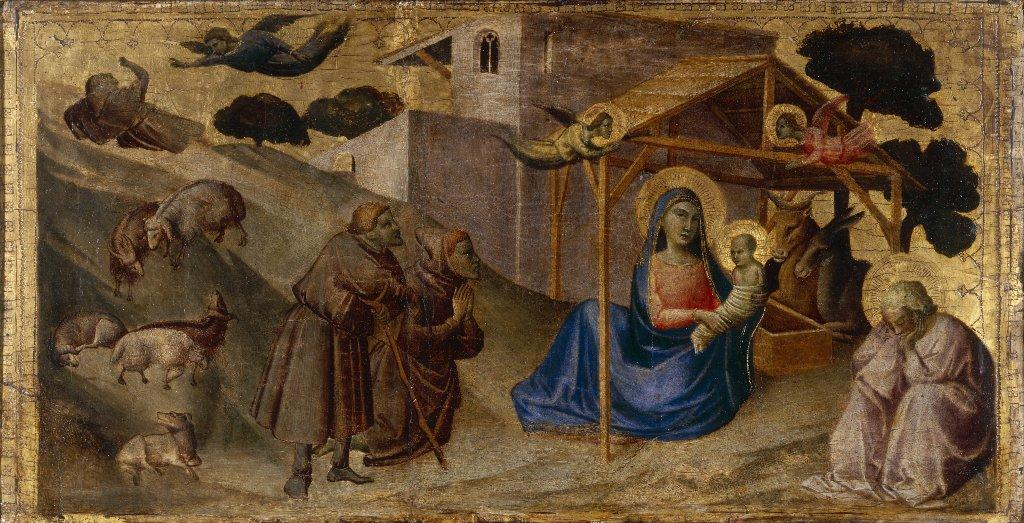
\includegraphics[width=1\textwidth]{annexes/figures/ptrGaddiAdoration.jpg}
    \caption{Taddeo Gaddi, \textit{L'Adoration des bergers}, vers 1330, tempéra sur bois, Dijon, Musée des Beaux-Arts, inv. 1470 © Musée des Beaux-Arts de Dijon}
    \label{fig:ptrGaddiAdoration}
\end{figure}


\begin{figure}[H]
    \centering
    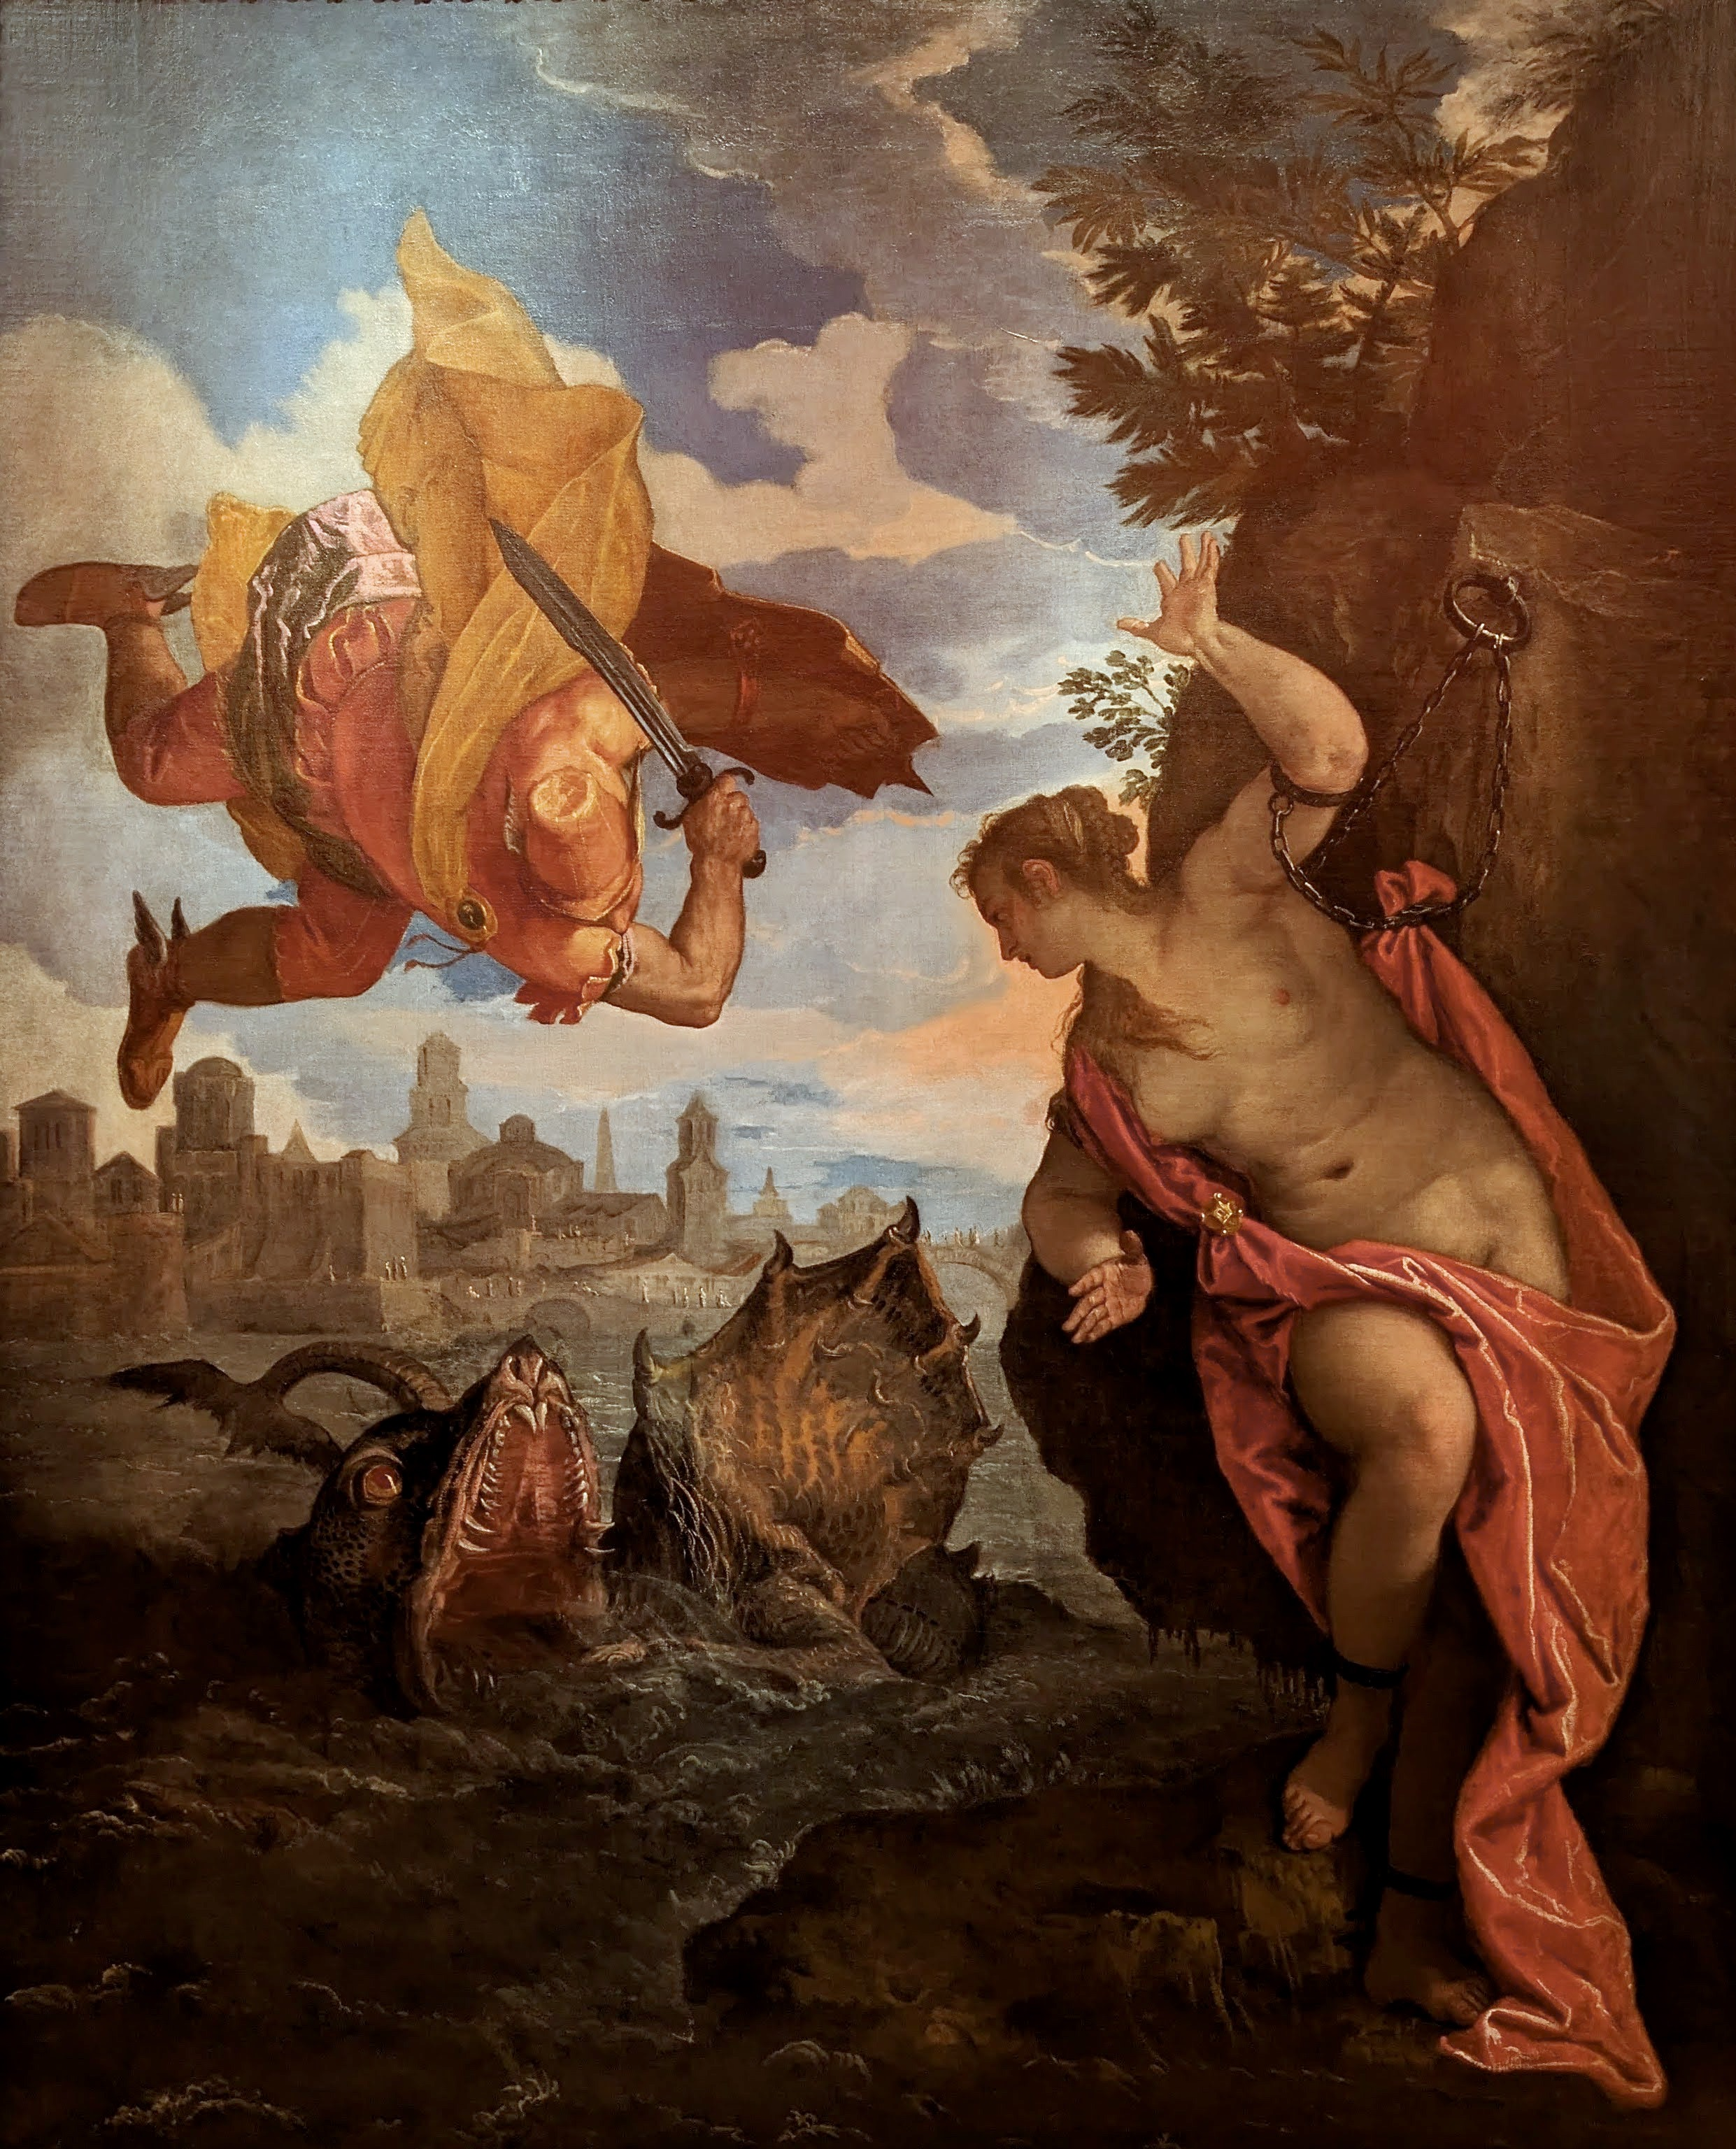
\includegraphics[height=0.4\textheight]{annexes/figures/ptrVeronesePersee.jpg}
    \caption{Paul Véronèse, \textit{Persée délivrant Andromède}, 1575-1580, peinture à l'huile sur toile, Rennes, Musée des Beaux-Arts de Rennes, inv. 801.1.1}
    \label{fig:ptrVeronesePersee}
\end{figure}

\begin{figure}[H]
    \centering
    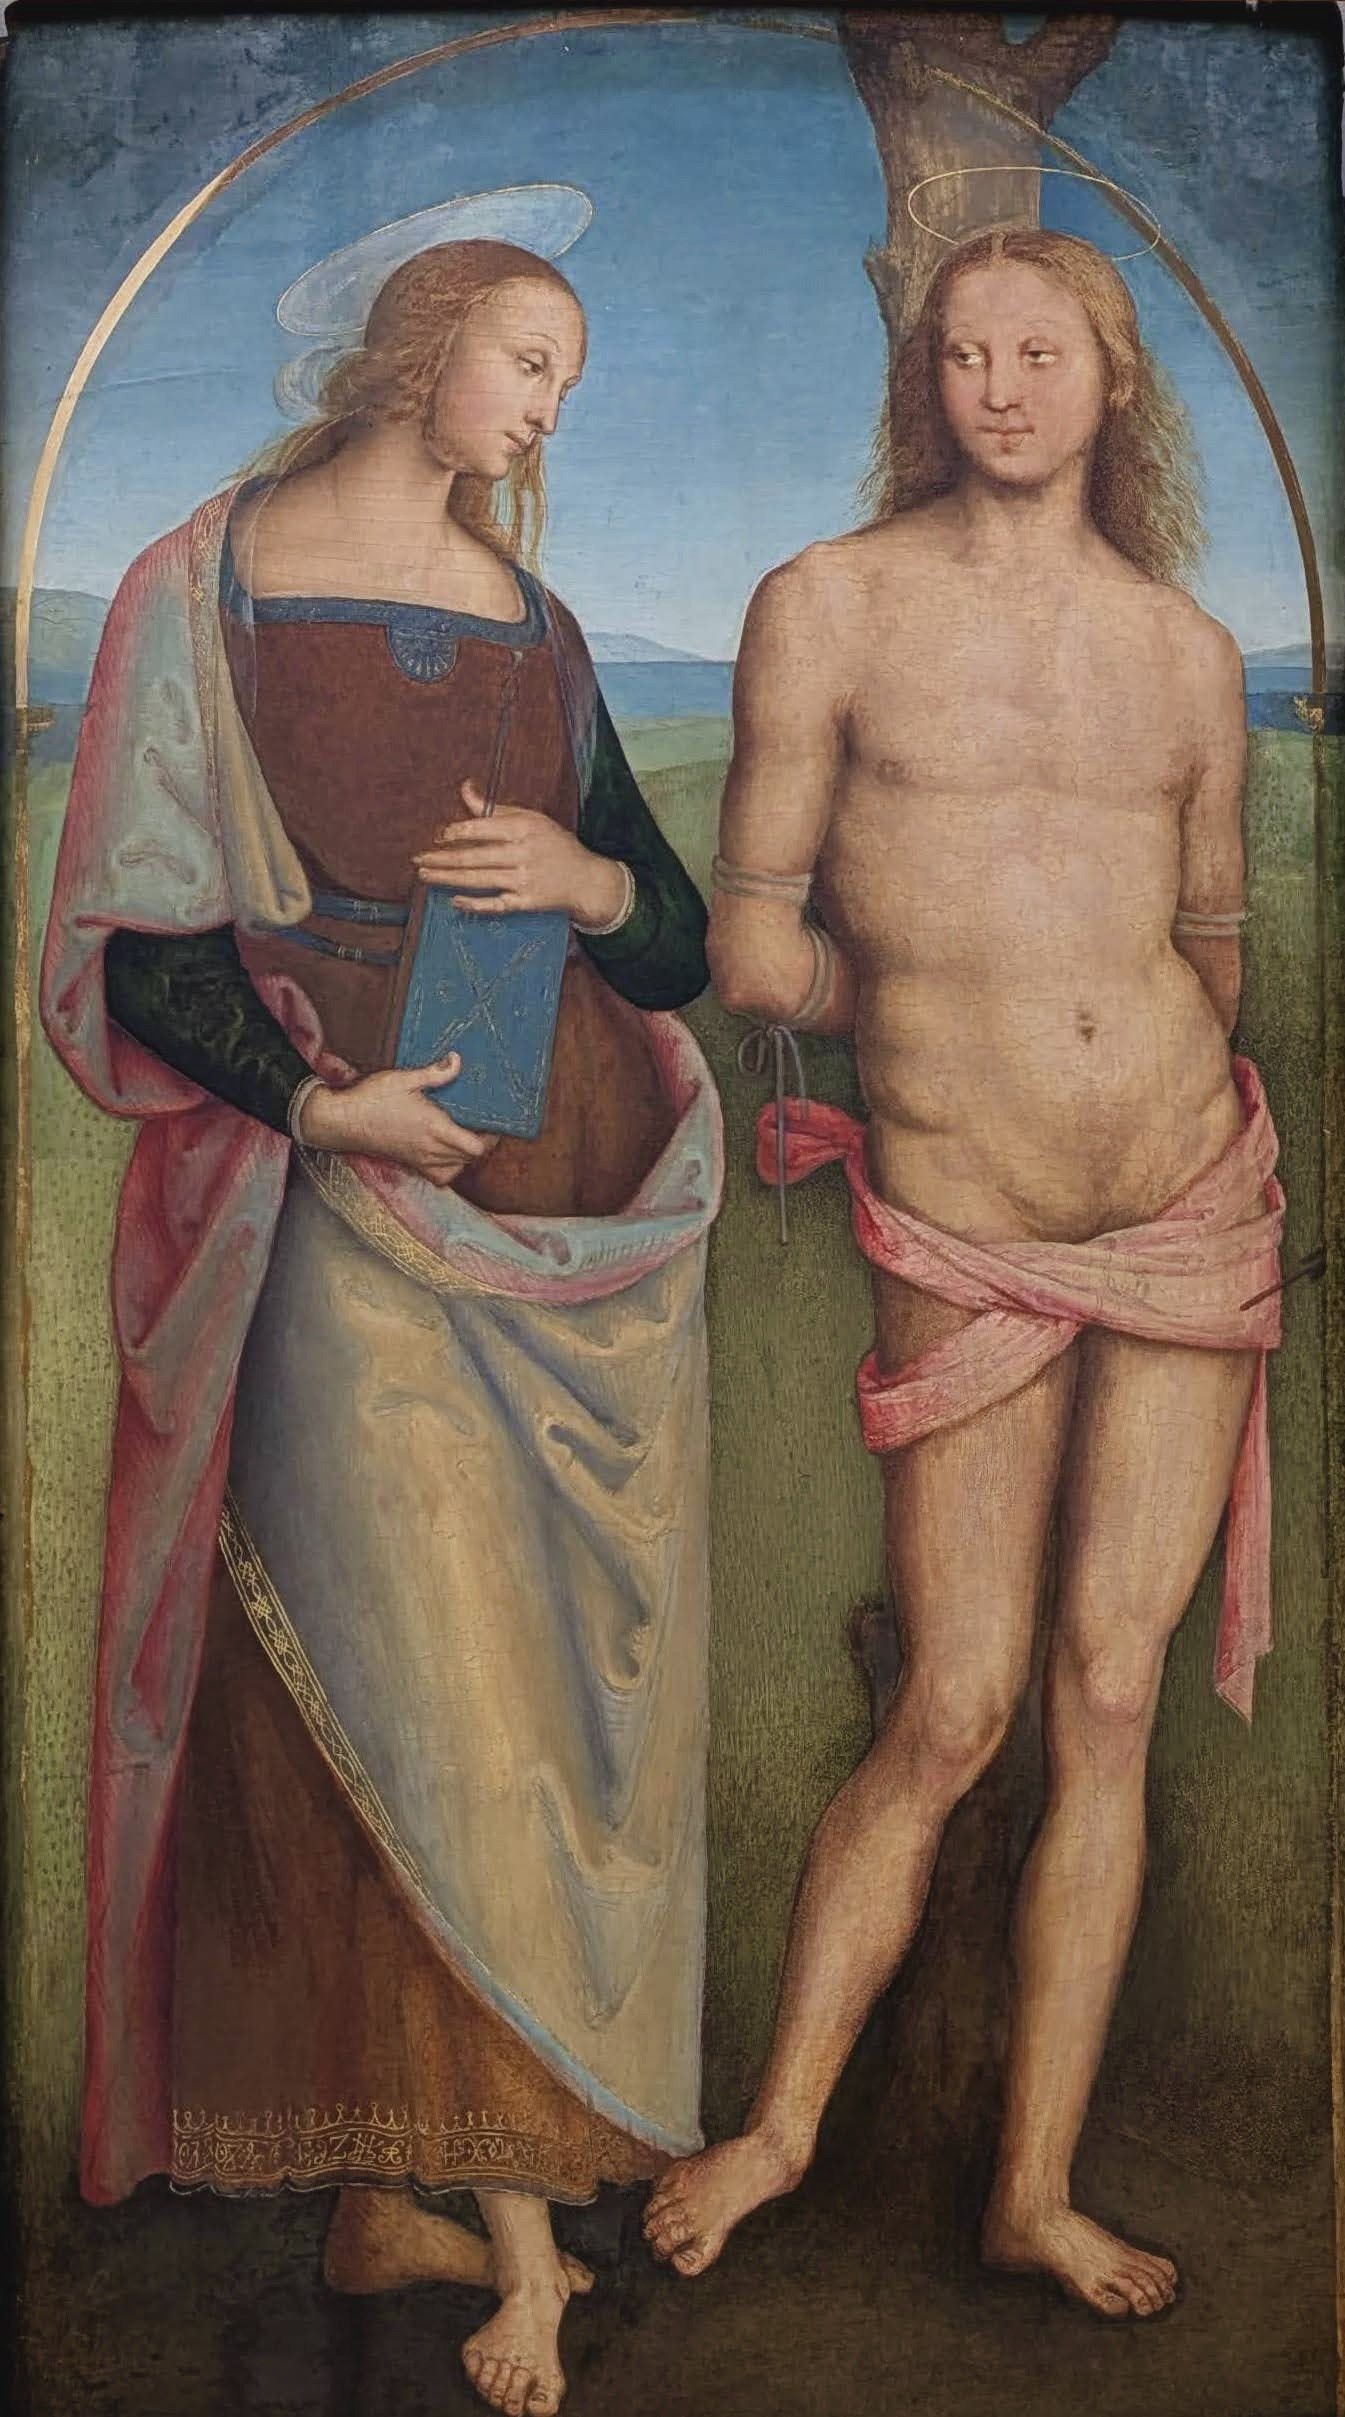
\includegraphics[height=0.4\textheight]{annexes/figures/ptrPeruginSaints.jpg}
    \caption{Pérugin, \textit{Saint Sébastien et sainte Apolline}, 1513 -1523, peinture à l'huile sur toile, Grenoble, Musée de Grenoble, inv. MG 48}
    \label{fig:ptrPeruginSaints}
\end{figure}

\begin{figure}[H]
    \centering
    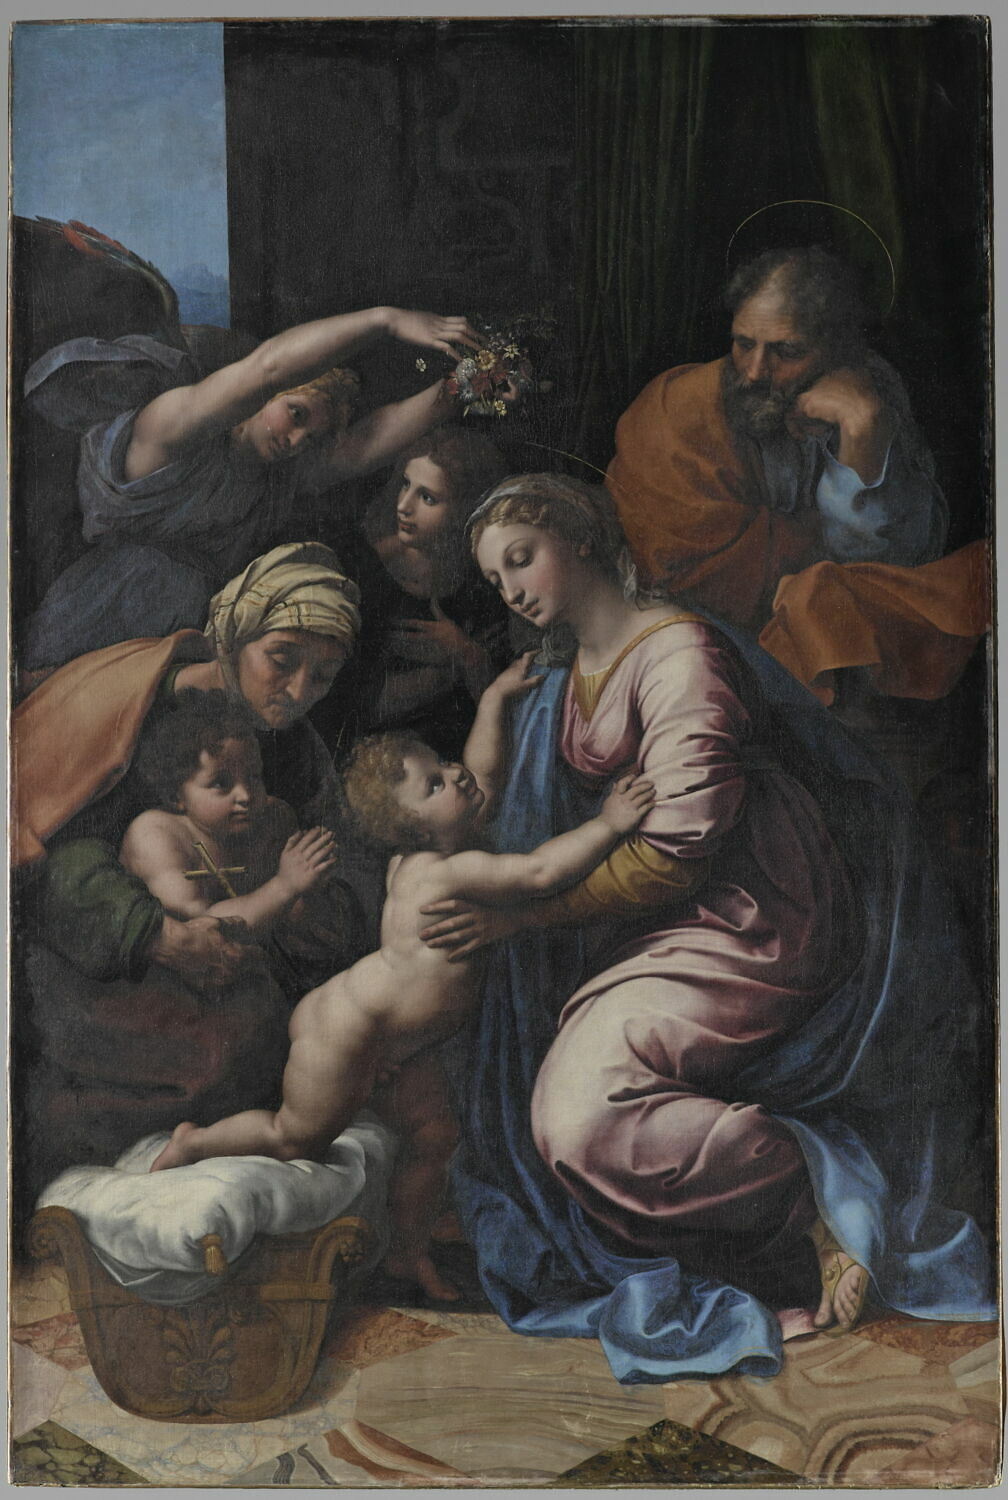
\includegraphics[height=0.4\textheight]{annexes/figures/ptrRaphaelSteFam.jpg}
    \caption{Raphaël, \textit{La Sainte Famille, dit La Grande Sainte Famille de François Ier}, 1518, peinture à l'huile sur toile, Paris, Musée du Louvre, INV 604 ; MR 432 © 2013 GrandPalaisRmn (musée du Louvre) / Adrien Didierjean}
    \label{fig:ptrRaphaelSteFam}
\end{figure}


\section{Exemples d'images inexploitables}

\begin{figure}[H]
    \centering
    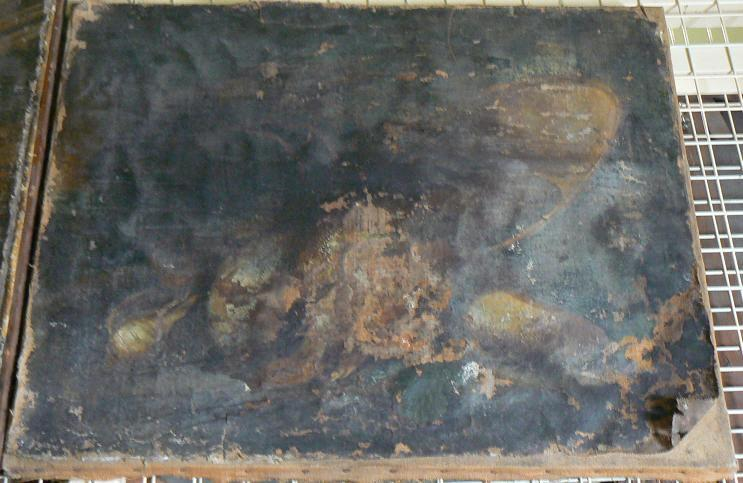
\includegraphics[height=0.3\textheight]{annexes/figures/ptrRecco.jpg}
    \caption{Giuseppe Recco \textit{Nature morte : poisson de mer et chaudron}, Musée des Beaux-Arts (Orléans), inv. 1173, Lien AGORHA : \\ \url{https://agorha.inha.fr/ark:/54721/d5fc162e-48a3-4508-9a6c-562fb76c1a1a}}
    \label{fig:ptrRecco}
\end{figure}


\begin{figure}[H]
    \centering
    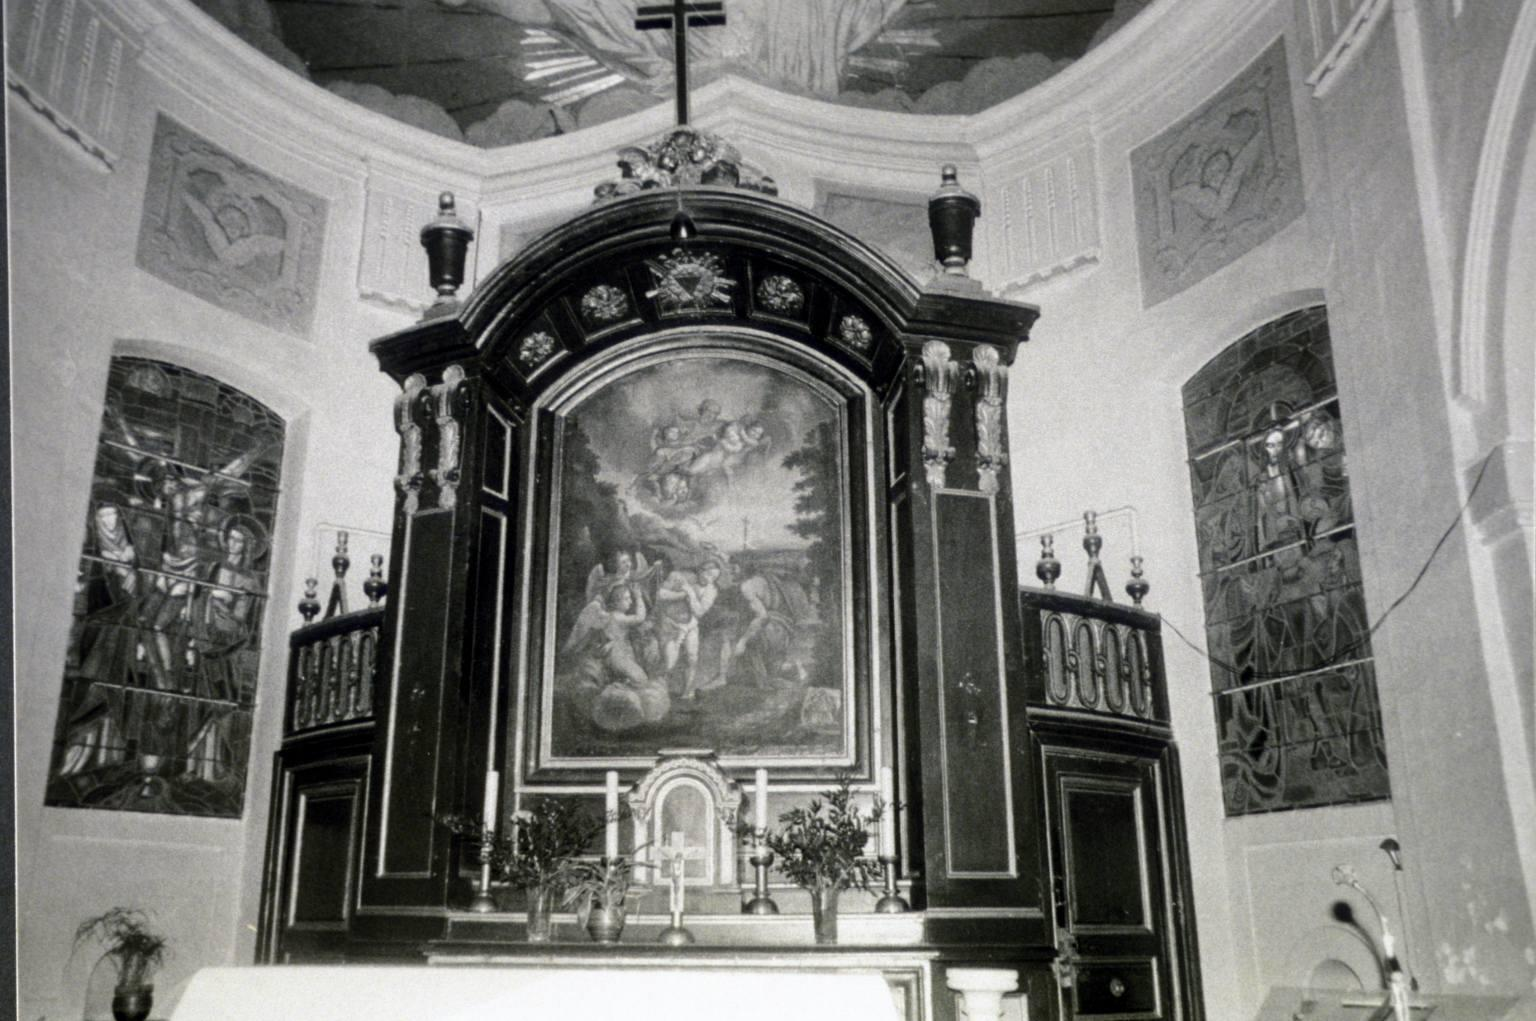
\includegraphics[height=0.4\textheight]{annexes/figures/ptrAlbani.jpg}
    \caption{Copie anonyme d'après Francesco Albani, \textit{Le Baptême du Christ}, Eglise Saint-Jean-Baptiste (Esbly), Lien AGORHA : \\ \url{https://agorha.inha.fr/ark:/54721/d9cc8098-0959-422e-902d-d5a8a6d41c6d}}
    \label{fig:ptrAlbani}
\end{figure}







\chapter[Visualisation du corpus]{Visualisation du corpus dans Pixplot et dans Panoptic}

\section{Métriques par classe}

\begin{figure}[H]
    \centering
    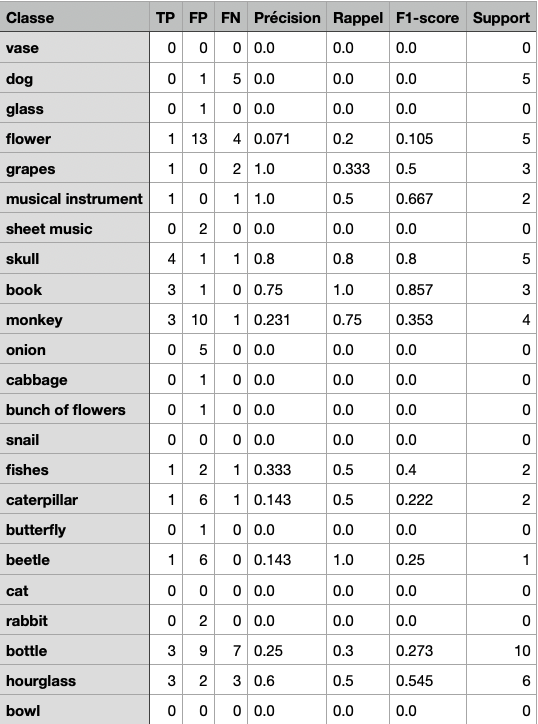
\includegraphics[width=0.5\textwidth]{annexes/tables/metricsYOLO1.png}
    \label{fig:YOLO1}
\end{figure}

\begin{figure}[H]
    \centering
    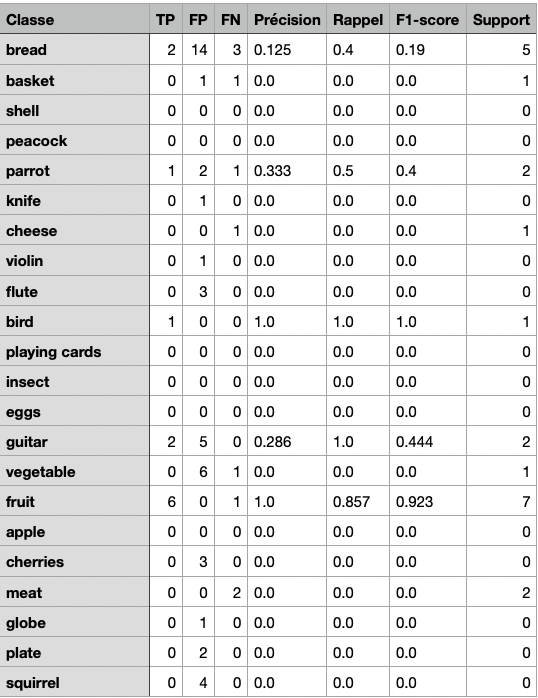
\includegraphics[width=0.5\textwidth]{annexes/tables/metricsYOLO2.png}
    \label{fig:YOLO2}
\end{figure}



\begin{minted}[frame=lines, linenos, fontsize=\small]{python}
import json
from rdflib import Graph, Namespace
from collections import defaultdict

"""
Ce script génère deux fichiers pour faciliter l’exploitation du thésaurus Garnier de l’INHA à partir d’un fichier XML-RDF :
- un fichier JSON qui représente la hiérarchie complète des concepts et qui inclut, pour chacun d'entre eux : l’URI (id), le label préféré (prefLabel), les labels alternatifs (altLabels), les concepts enfants (children). La hiérarchie est structurée sous forme de dictionnaires imbriqués, et tous les concepts sont triés par ordre alphabétique.

- un fichier TXT qui contient uniquement les labels principaux (prefLabel) des concepts. La hiérarchie est reproduite grâce à une indentation par niveau.
"""

rdf_entree = "thesaurusGarnierINHA.rdf"
resultat_json = "JSONthesaurusGarnierINHA.json"
resultat_txt = "TXTthesaurusGarnierINHA.txt"

# Charger le fichier XML-RDF
g = Graph()
g.parse(rdf_entree, format="xml")

# définition du namespace SKOS
SKOS = Namespace("http://www.w3.org/2004/02/skos/core#")

# préparation des dictionnaires
labels = {}
alt_labels = defaultdict(list)
broader_relations = defaultdict(list)

# Extraction des "prefLabel"
for s, p, o in g.triples((None, SKOS.prefLabel, None)):
    labels[str(s)] = str(o)

# Extraction des "altLabel"
for s, p, o in g.triples((None, SKOS.altLabel, None)):
    alt_labels[str(s)].append(str(o))

# identification de la hierarchie parents enfants des concepts
for s, p, o in g.triples((None, SKOS.broader, None)):
    broader_relations[str(o)].append(str(s))

# Trouver les concepts racines (càd les concepts sans skos:broader)
all_concepts = set(labels.keys()) | set(alt_labels.keys())
children = set()
for children_list in broader_relations.values():
    children.update(children_list)

roots = list(all_concepts - children)

# fonction récursive pour créer la hiérarchie JSON
def build_hierarchy(concept_uri):
    children_sorted = sorted(
        broader_relations.get(concept_uri, []),
        key=lambda x: labels.get(x, "").lower()
    )
    return {
        "id": concept_uri,
        "label": labels.get(concept_uri, ""),
        "altLabels": sorted(alt_labels.get(concept_uri, []), key=str.lower),
        "children": [build_hierarchy(child) for child in children_sorted]
    }

# Créer la hiérarchie complète (racines triées dans l'ordre alphabétique des labels)
roots_sorted = sorted(roots, key=lambda x: labels.get(x, "").lower())
hierarchy = [build_hierarchy(root) for root in roots_sorted]

# Sauvegarder en JSON
with open(resultat_json, "w", encoding="utf-8") as f:
    json.dump(hierarchy, f, ensure_ascii=False, indent=2)
print(f"{resultat_json} a bien été créé !")

# Sauvegarde d'un txt indenté contenant seulement les labels
def write_txt(node, f, indent=0):
    f.write("\t" * indent + str(node["label"]) + "\n")
    for child in node["children"]:
        write_txt(child, f, indent + 1)

with open(resultat_txt, "w", encoding="utf-8") as f:
    for root in hierarchy:
        write_txt(root, f)
print(f"{resultat_txt} a bien été créé !")
\end{minted}

\section{Visualisation du corpus dans PixPlot}

\begin{figure}[H]
    \centering
    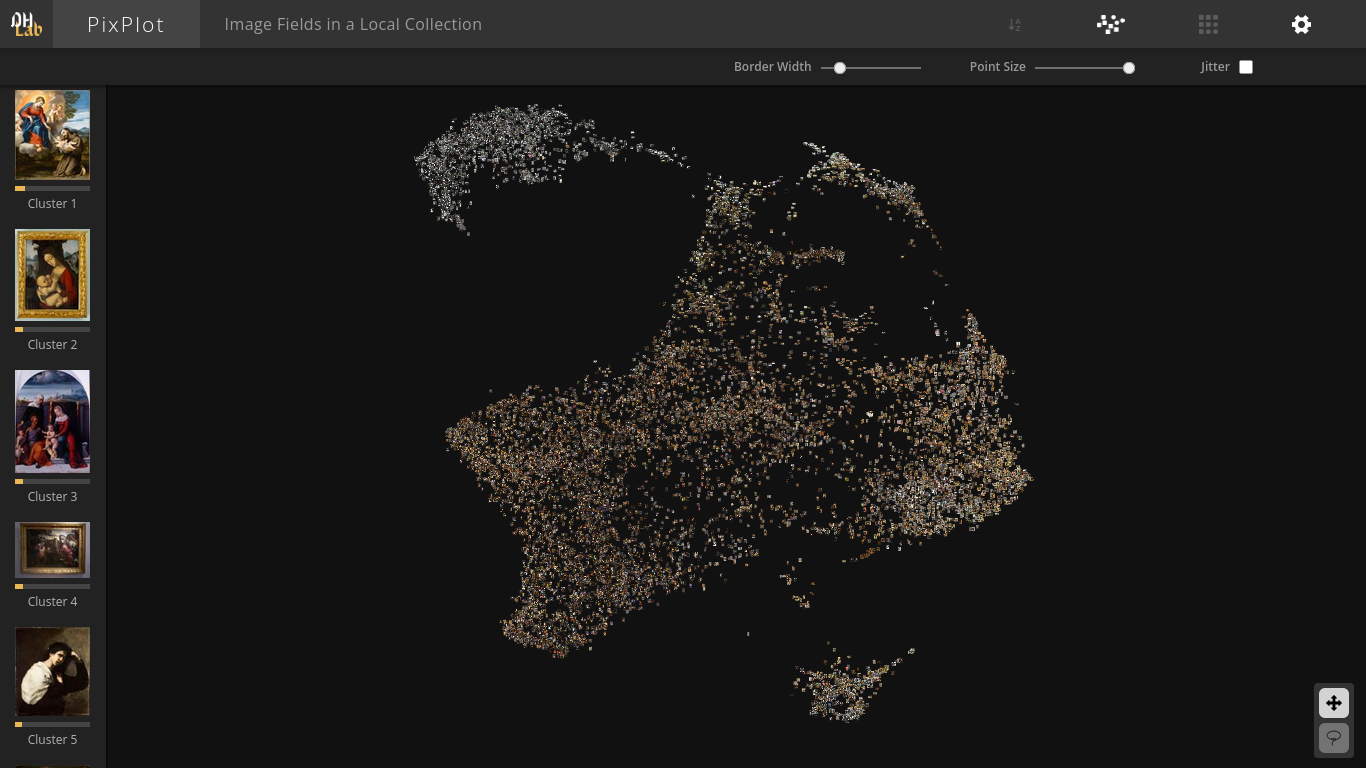
\includegraphics[width=1\textwidth]{annexes/figures/PP-generale.png}
    \caption{Visualisation générale des tableaux du RETIF dans PixPlot.}
    \label{fig:PP-general}
\end{figure}

\begin{figure}[H]
    \centering
    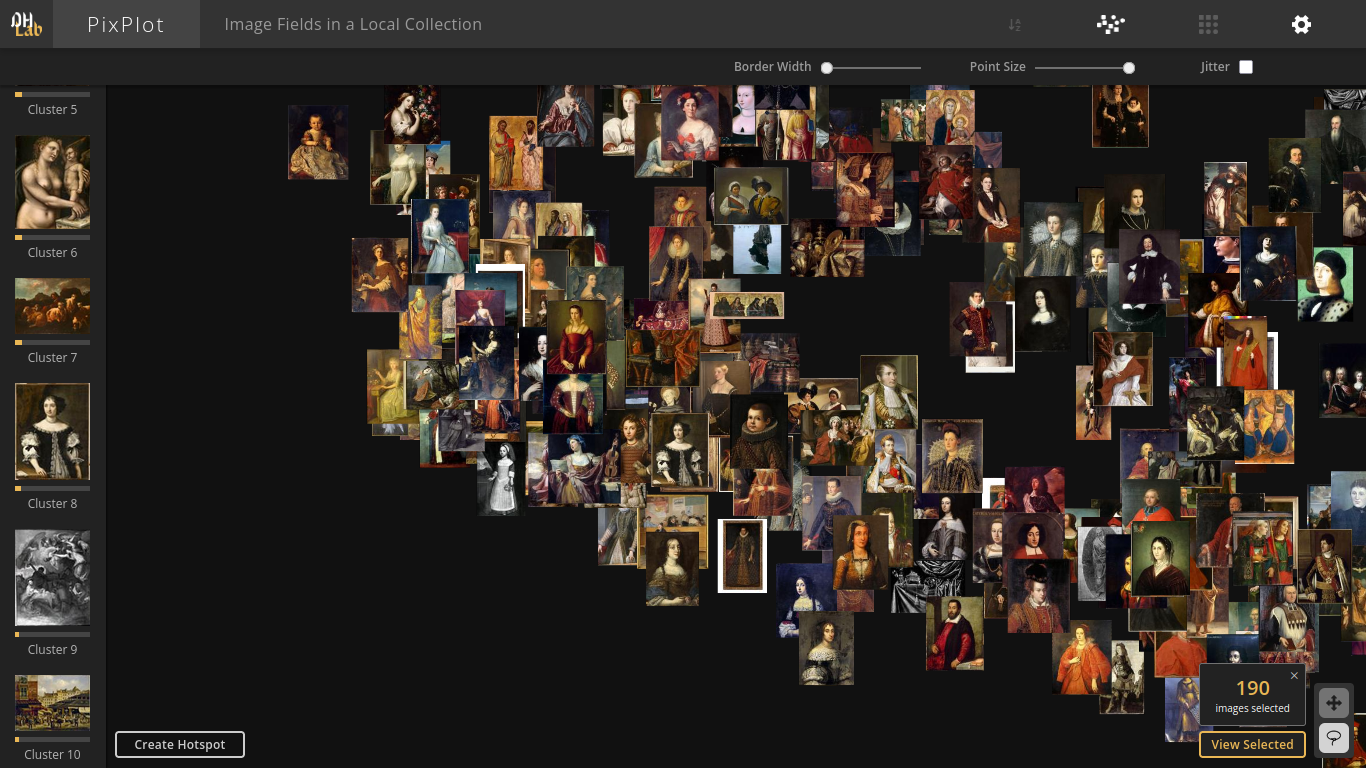
\includegraphics[width=1\textwidth]{annexes/figures/PP-portraits.png}
    \caption{Cluster de portraits identifié dans l'angle inférieur gauche de la visualisation du RETIF dans PixPlot.}
    \label{fig:PP-portraits}
\end{figure}

\begin{figure}[H]
    \centering
    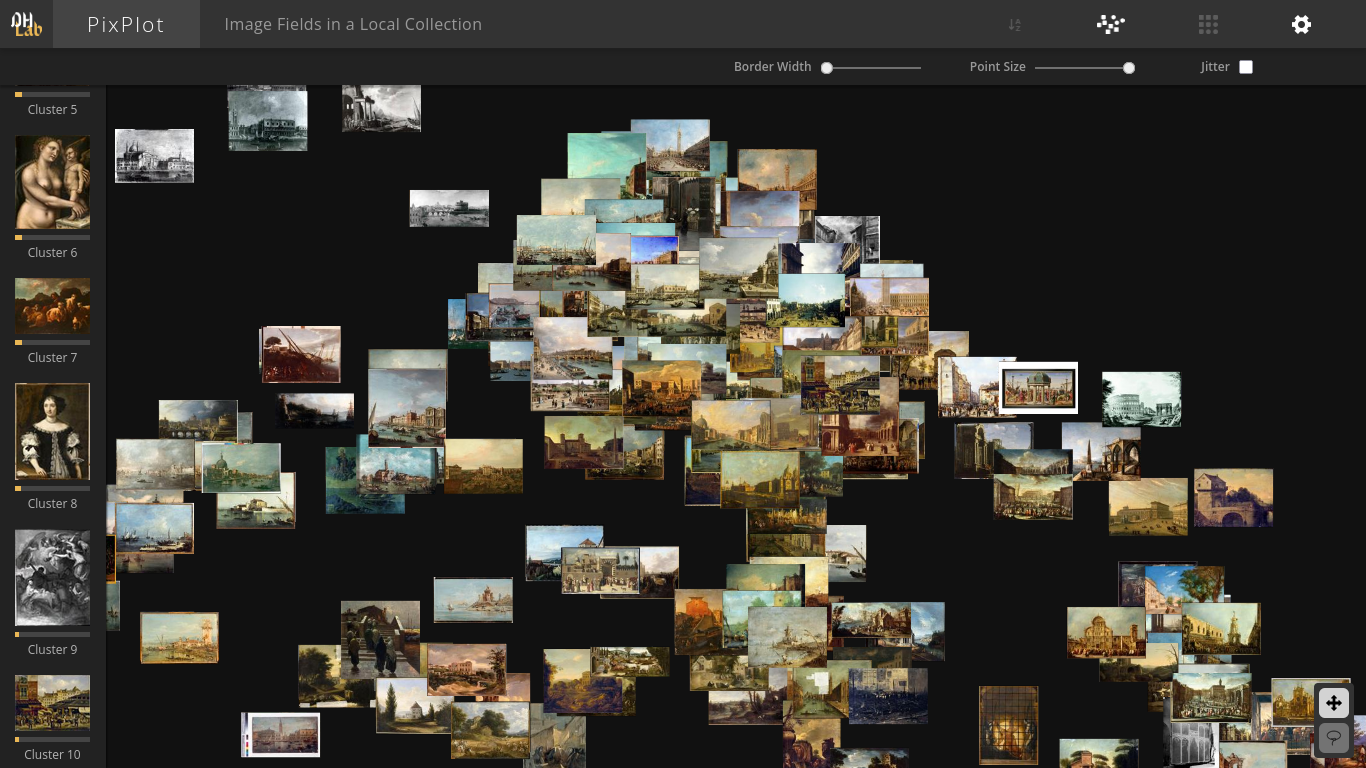
\includegraphics[width=1\textwidth]{annexes/figures/PP-vedute.png}
    \caption{Cluster de paysages urbains dans l'angle supérieur droit de la visualisation du RETIF dans PixPlot.}
    \label{fig:PP-vedute}
\end{figure}

\begin{figure}[H]
    \centering
    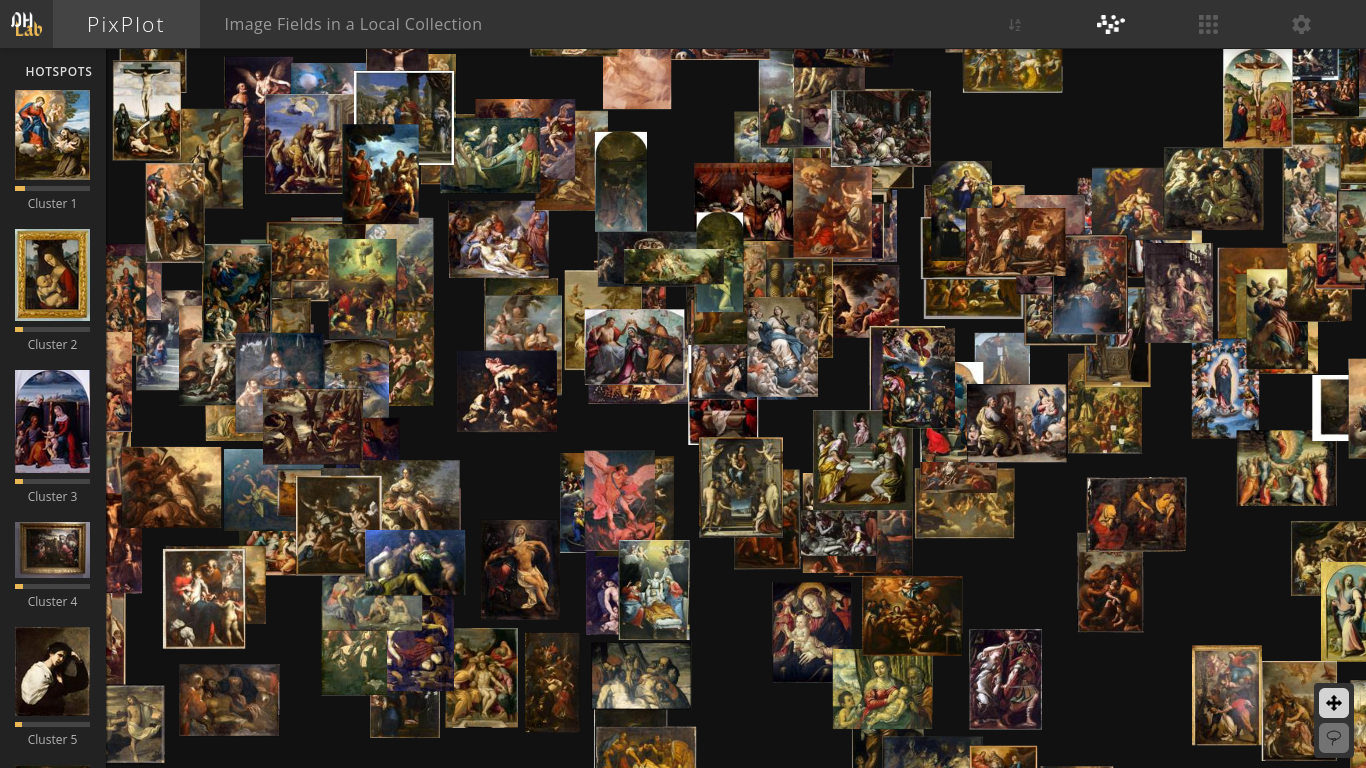
\includegraphics[width=1\textwidth]{annexes/figures/PP-scenes.png}
    \caption{Cluster des scènes religieuses et mythologiques au centre de la visualisation du RETIF dans PixPlot.}
    \label{fig:PP-scenes}
\end{figure}

\begin{figure}[H]
    \centering
    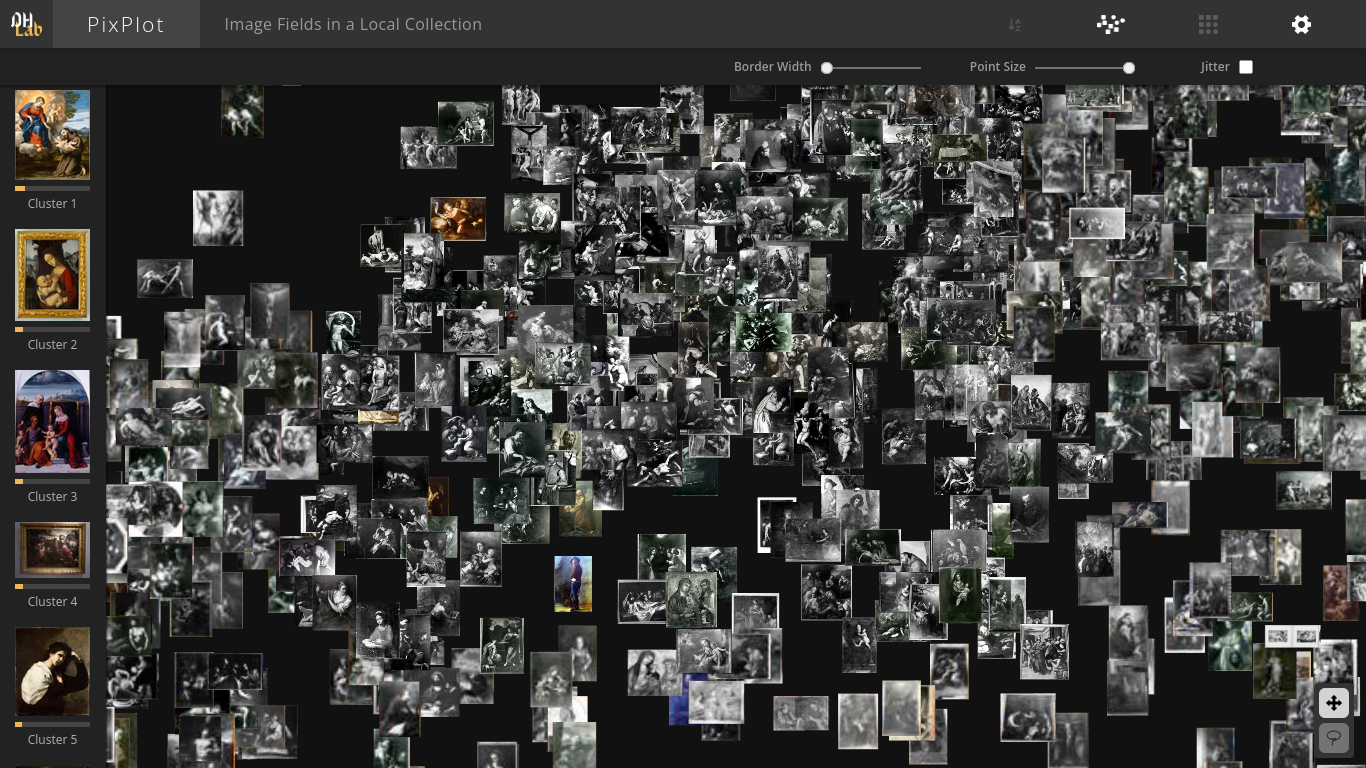
\includegraphics[width=1\textwidth]{annexes/figures/PP-n&b.png}
    \caption{Cluster des photographies en noir et blanc dans l'angle supérieur gauche de la visualisation du RETIF dans PixPlot.}
    \label{fig:PP-n&b}
\end{figure}

\begin{figure}[H]
    \centering
    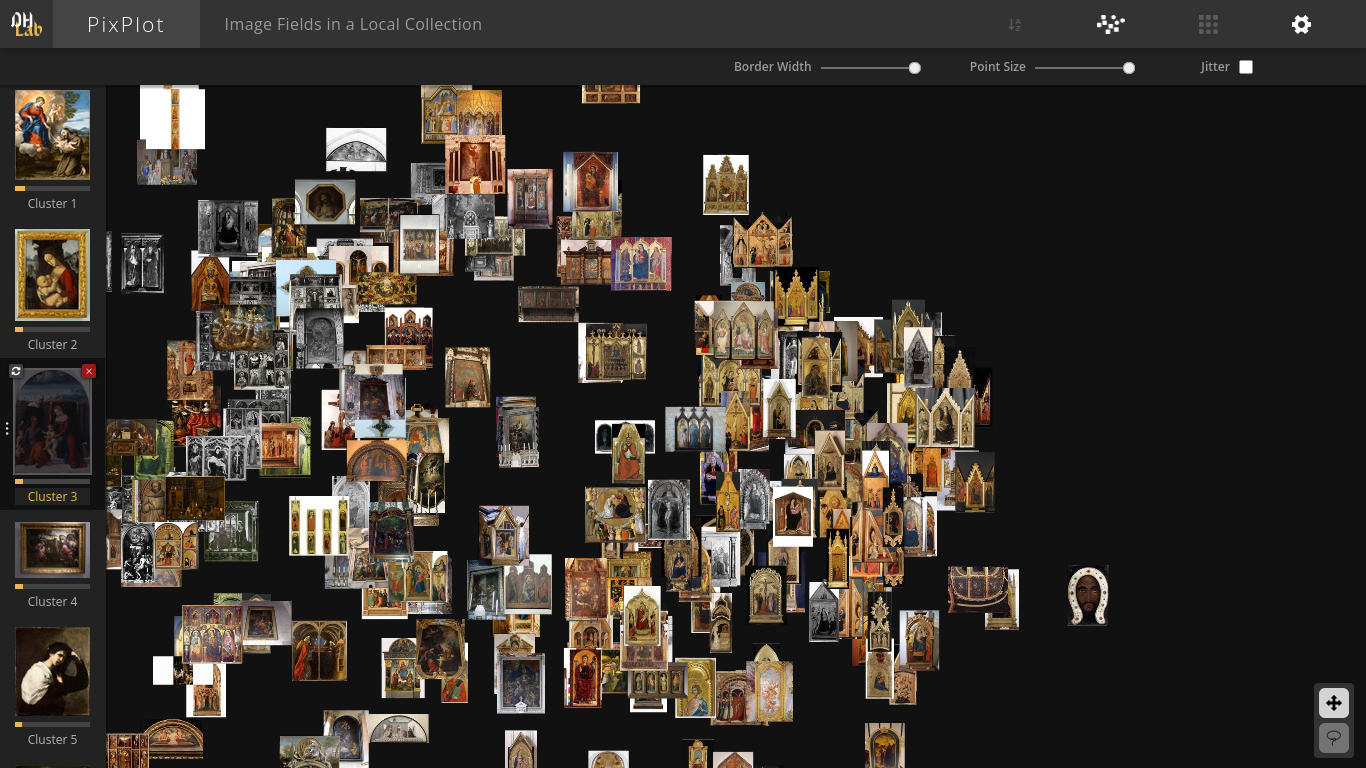
\includegraphics[width=1\textwidth]{annexes/figures/PP-polyptiques.png}
    \caption{Cluster des panneaux médiévaux et des tableaux dans leur contexte dans le bord droit  de la visualisation du RETIF dans PixPlot.}
    \label{fig:PP-polyptiques}
\end{figure}

\begin{figure}[H]
    \centering
    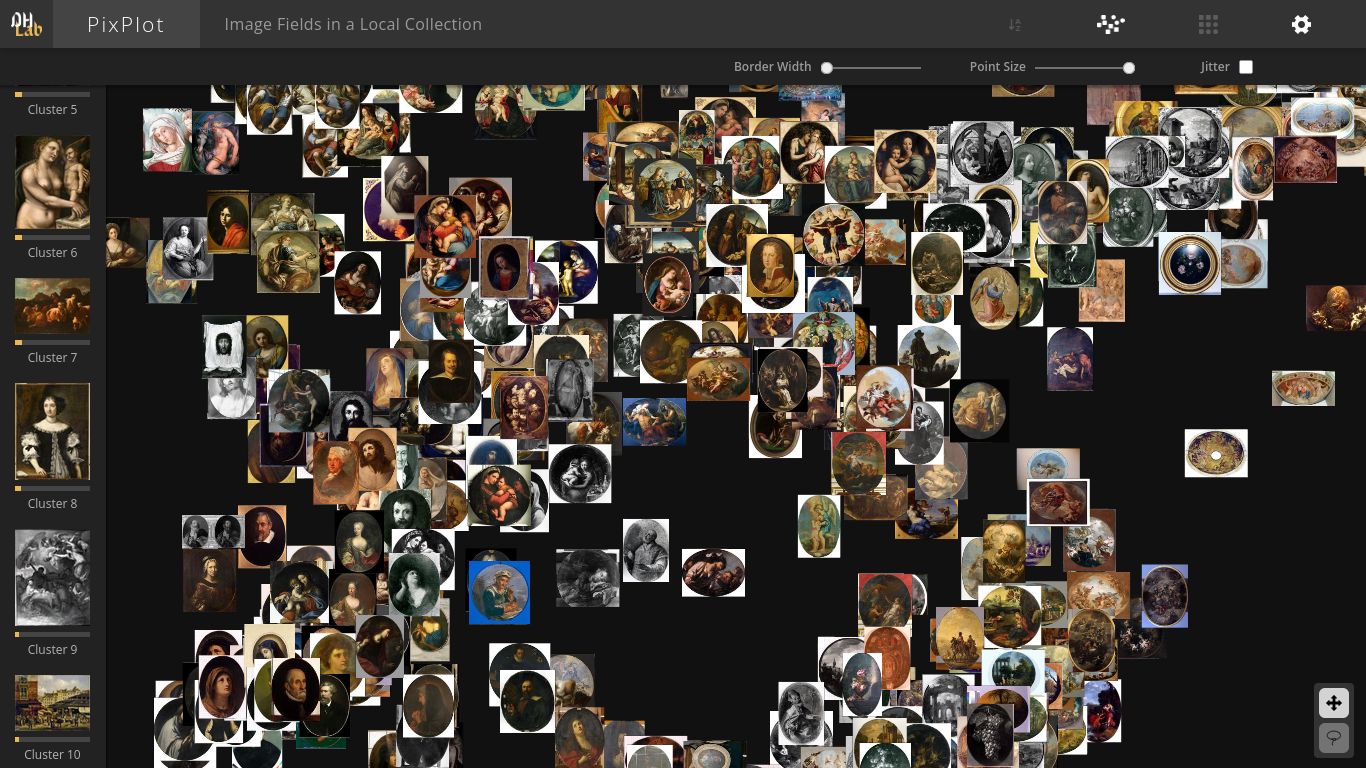
\includegraphics[width=1\textwidth]{annexes/figures/PP-ronds.png}
    \caption{Cluster des tableaux aux formats inhabituels (circulaire, ovale, hexagonal) dans l'angle inférieur droit de la visualisation du RETIF dans PixPlot.}
    \label{fig:PP-ronds}
\end{figure}

\section{Visualisation du corpus dans Panoptic}

\begin{figure}[H]
    \centering
    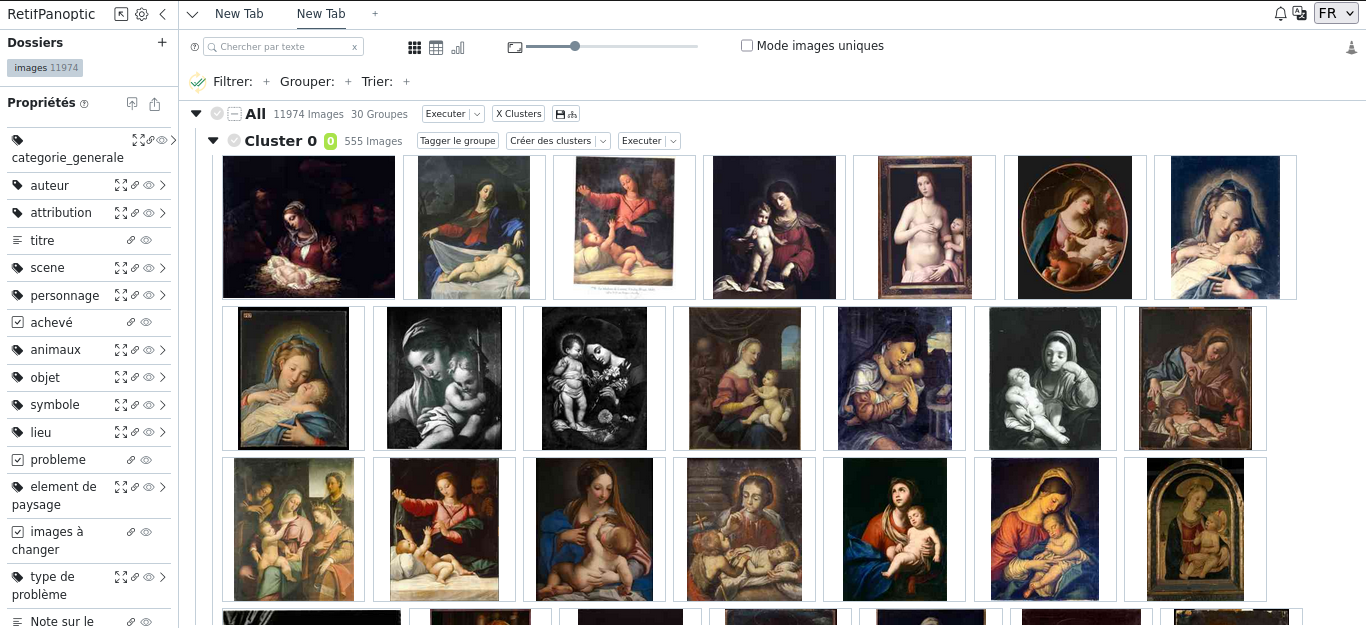
\includegraphics[width=1\textwidth]{annexes/figures/Pa-Vierges.png}
    \caption{Cluster des Vierge à l'Enfant dans Panoptic.}
    \label{fig:Pa-Vierges}
\end{figure}


\newpage{\pagestyle{empty}\cleardoublepage}

%%%%%%%%%%%%%%%%%%

\backmatter % glossaire, index, table des figures, table des matières.. (la bibliographie a déjà été appelée)

%\printindex
%\printglossaries[title=Glossaire]
%\listoftables
%\listoffigures
\tableofcontents
\end{document}
